%%%%%%%%%%%%%%%%%%%%%%%%%%%%%%%%%%%%%%%%%
% Beamer Presentation
% LaTeX Template
% Version 1.0 (10/11/12)
%
% This template has been downloaded from:
% http://www.LaTeXTemplates.com
%
% License:
% CC BY-NC-SA 3.0 (http://creativecommons.org/licenses/by-nc-sa/3.0/)
%
%%%%%%%%%%%%%%%%%%%%%%%%%%%%%%%%%%%%%%%%%

%----------------------------------------------------------------------------------------
%	PACKAGES AND THEMES
%----------------------------------------------------------------------------------------

\documentclass{beamer}

\mode<presentation> {

% The Beamer class comes with a number of default slide themes
% which change the colors and layouts of slides. Below this is a list
% of all the themes, uncomment each in turn to see what they look like.

%\usetheme{default}
%\usetheme{AnnArbor}
%\usetheme{Antibes}
%\usetheme{Bergen}
%\usetheme{Berkeley}
%\usetheme{Berlin}
%\usetheme{Boadilla}
%\usetheme{CambridgeUS}
%\usetheme{Copenhagen}
%\usetheme{Darmstadt}
%\usetheme{Dresden}
%\usetheme{Frankfurt}
%\usetheme{Goettingen}
%\usetheme{Hannover}
%\usetheme{Ilmenau}
%\usetheme{JuanLesPins}
%\usetheme{Luebeck}
%\usetheme{Madrid}
%\usetheme{Malmoe}
%\usetheme{Marburg}
%\usetheme{Montpellier}
%\usetheme{PaloAlto}
%\usetheme{Pittsburgh}
%\usetheme{Rochester}
%\usetheme{Singapore}
%\usetheme{Szeged}
%\usetheme{Warsaw}
\usetheme{Amsterdam}

% As well as themes, the Beamer class has a number of color themes
% for any slide theme. Uncomment each of these in turn to see how it
% changes the colors of your current slide theme.

%\usecolortheme{albatross}
%\usecolortheme{beaver}
%\usecolortheme{beetle}
%\usecolortheme{crane}
%\usecolortheme{dolphin}
%\usecolortheme{dove}
%\usecolortheme{fly}
%\usecolortheme{lily}
%\usecolortheme{orchid}
%\usecolortheme{rose}
%\usecolortheme{seagull}
%\usecolortheme{seahorse}
%\usecolortheme{whale}
%\usecolortheme{wolverine}

%\setbeamertemplate{footline} % To remove the footer line in all slides uncomment this line
%\setbeamertemplate{footline}[page number] % To replace the footer line in all slides with a simple slide count uncomment this line

%\setbeamertemplate{navigation symbols}{} % To remove the navigation symbols from the bottom of all slides uncomment this line
}
\usepackage{multimedia}
\usepackage{graphicx} % Allows including images
\usepackage{booktabs} % Allows the use of \toprule, \midrule and \bottomrule in tables
\usepackage[utf8]{inputenc}
% http://tex.stackexchange.com/questions/107637/repeated-division-converting-from-base-10-to-another-base


\newcount\total
\newcount\lasttotal
\newcount\targetbase

\def\digittoalpha#1{%
    \ifcase#1\relax0\or1\or2\or3\or4\or5\or6\or7\or8\or9%
    \or a\or b\or c\or d\or e\or f\or g\or h\or i\or j\or k\or l\or m%
    \or n\or p\or p\or q\or r\or s\or t\or u\or v\or w\or x\or y\or z\else?\fi%
}

\def\baseconversiontable#1#2{%
    \begin{tikzpicture}[every node/.style={minimum width=1cm, minimum height=0.5cm}, x=1cm,y=0.5cm]
    %
    \total=#1%
    \targetbase=#2
    \def\newnumber{}
    %
    \pgfmathloop
    \ifnum\total<1
    \else
        %
        \ifnum\pgfmathcounter>1
            \node at (\pgfmathcounter, -\pgfmathcounter+1) (tmp) {\the\targetbase};
            \draw (tmp.north west) |- (tmp.south east);
            %
            \node at (\pgfmathcounter-1, -\pgfmathcounter) (tmp) {\pgfmathparse{int(-\total*\targetbase)}\pgfmathresult};
            \draw (tmp.south west) -- (tmp.south east);
            %
            \pgfmathparse{int(\lasttotal-\total*\targetbase)}%
            \let\digit=\pgfmathresult
            \node at (\pgfmathcounter-1, -\pgfmathcounter-1) [text=red] {\digit};
            \edef\newnumber{\digit\newnumber}
        \fi
        %
        \ifnum\total<\targetbase
            \edef\currentdigit{\uppercase{\digittoalpha{\the\total}}}%
            \edef\newnumber{\currentdigit\newnumber}
            \ifnum\total>9
              \edef\currentdigit{\noexpand\rm{\currentdigit}}%
            \fi
            \node at (\pgfmathcounter, -\pgfmathcounter) [text=red]  {\the\total};
            %\color{black}\the\total(\color{red}\currentdigit\color{black})
            %};
        \else
            \node at (\pgfmathcounter, -\pgfmathcounter) {\the\total};
        \fi
        \lasttotal=\total
        \divide\total by\targetbase
    \repeatpgfmathloop    
    \draw [->] (\pgfmathcounter-1,-\pgfmathcounter-1) -- ++(-0.5,0); 
    %\node [anchor=west] at (1, -\pgfmathcounter-2) {$#1=\newnumber_{\the\targetbase}$};
    \end{tikzpicture}   
}



\usepackage{framed}

\usepackage{algorithm}
\usepackage[noend]{algpseudocode}
\definecolor{algocoul}{rgb}{0,0,0.75}
\definecolor{algocom}{rgb}{.75,.25,0}
\floatname{algorithm}{Algorithme}

\usepackage{tikz}
\usepackage{tikz-timing}
\usepackage{tkz-graph} 
\usetikzlibrary{arrows,shapes.gates.logic.US,shapes.gates.logic.IEC,calc,shapes.geometric,positioning}
\tikzset{
  multiplexer/.style={
    draw,
    trapezium,
    shape border uses incircle, 
    shape border rotate=270,
    minimum size=18pt
  }  
}

\tikzset{
    alu/.style={trapezium,
            trapezium angle=26,
            shape border rotate=180,
            minimum width=3cm,
            minimum height=2cm,
            trapezium stretches=true,
            append after command={%
                    \pgfextra
                        \draw (\tikzlastnode.top left corner) --
                           (\tikzlastnode.top right corner) -- 
                           (\tikzlastnode.bottom right corner) -- 
                           ($(\tikzlastnode.bottom right corner)!.666!(\tikzlastnode.bottom side)$)--
                           ([yshift=-1cm]\tikzlastnode.bottom side)--
                           ($(\tikzlastnode.bottom side)!.334!(\tikzlastnode.bottom left corner)$)--
                           (\tikzlastnode.bottom left corner)--
                           (\tikzlastnode.top left corner);
                    \endpgfextra}},
}




\usepackage[europeanresistors, siunitx]{circuitikz}

%----------------------------------------------------------------------------------------
%	TITLE PAGE
%----------------------------------------------------------------------------------------

\title[Architecture]{Architecture des ordinateurs} % The short title appears at the bottom of every slide, the full title is only on the title page

\author{Jérémy Fix} % Your name
\institute[CS] % Your institution as it will appear on the bottom of every slide, may be shorthand to save space
{
CentraleSupélec \\ % Your institution for the title page
\medskip
\textit{jeremy.fix@centralesupelec.fr} % Your email address
}
\date{2017-2018} % Date, can be changed to a custom date

\begin{document}

\begin{frame}
\titlepage % Print the title page as the first slide
\end{frame}

%% \begin{frame}
%% \frametitle{Overview} % Table of contents slide, comment this block out to remove it
%% \tableofcontents % Throughout your presentation, if you choose to use \section{} and \subsection{} commands, these will automatically be printed on this slide as an overview of your presentation
%% \end{frame}

%----------------------------------------------------------------------------------------
%	PRESENTATION SLIDES
%----------------------------------------------------------------------------------------

%------------------------------------------------
\section{Introduction} % Sections can be created in order to organize your presentation into discrete blocks, all sections and subsections are automatically printed in the table of contents as an overview of the talk
%------------------------------------------------

\begin{frame}
\begin{center}
Architecture des ordinateurs
\end{center}
ou plutôt
\begin{center}
Réalisation \textbf{électronique} d'une machine \textbf{programmable} manipulant des représentations \textbf{numériques}
\end{center}
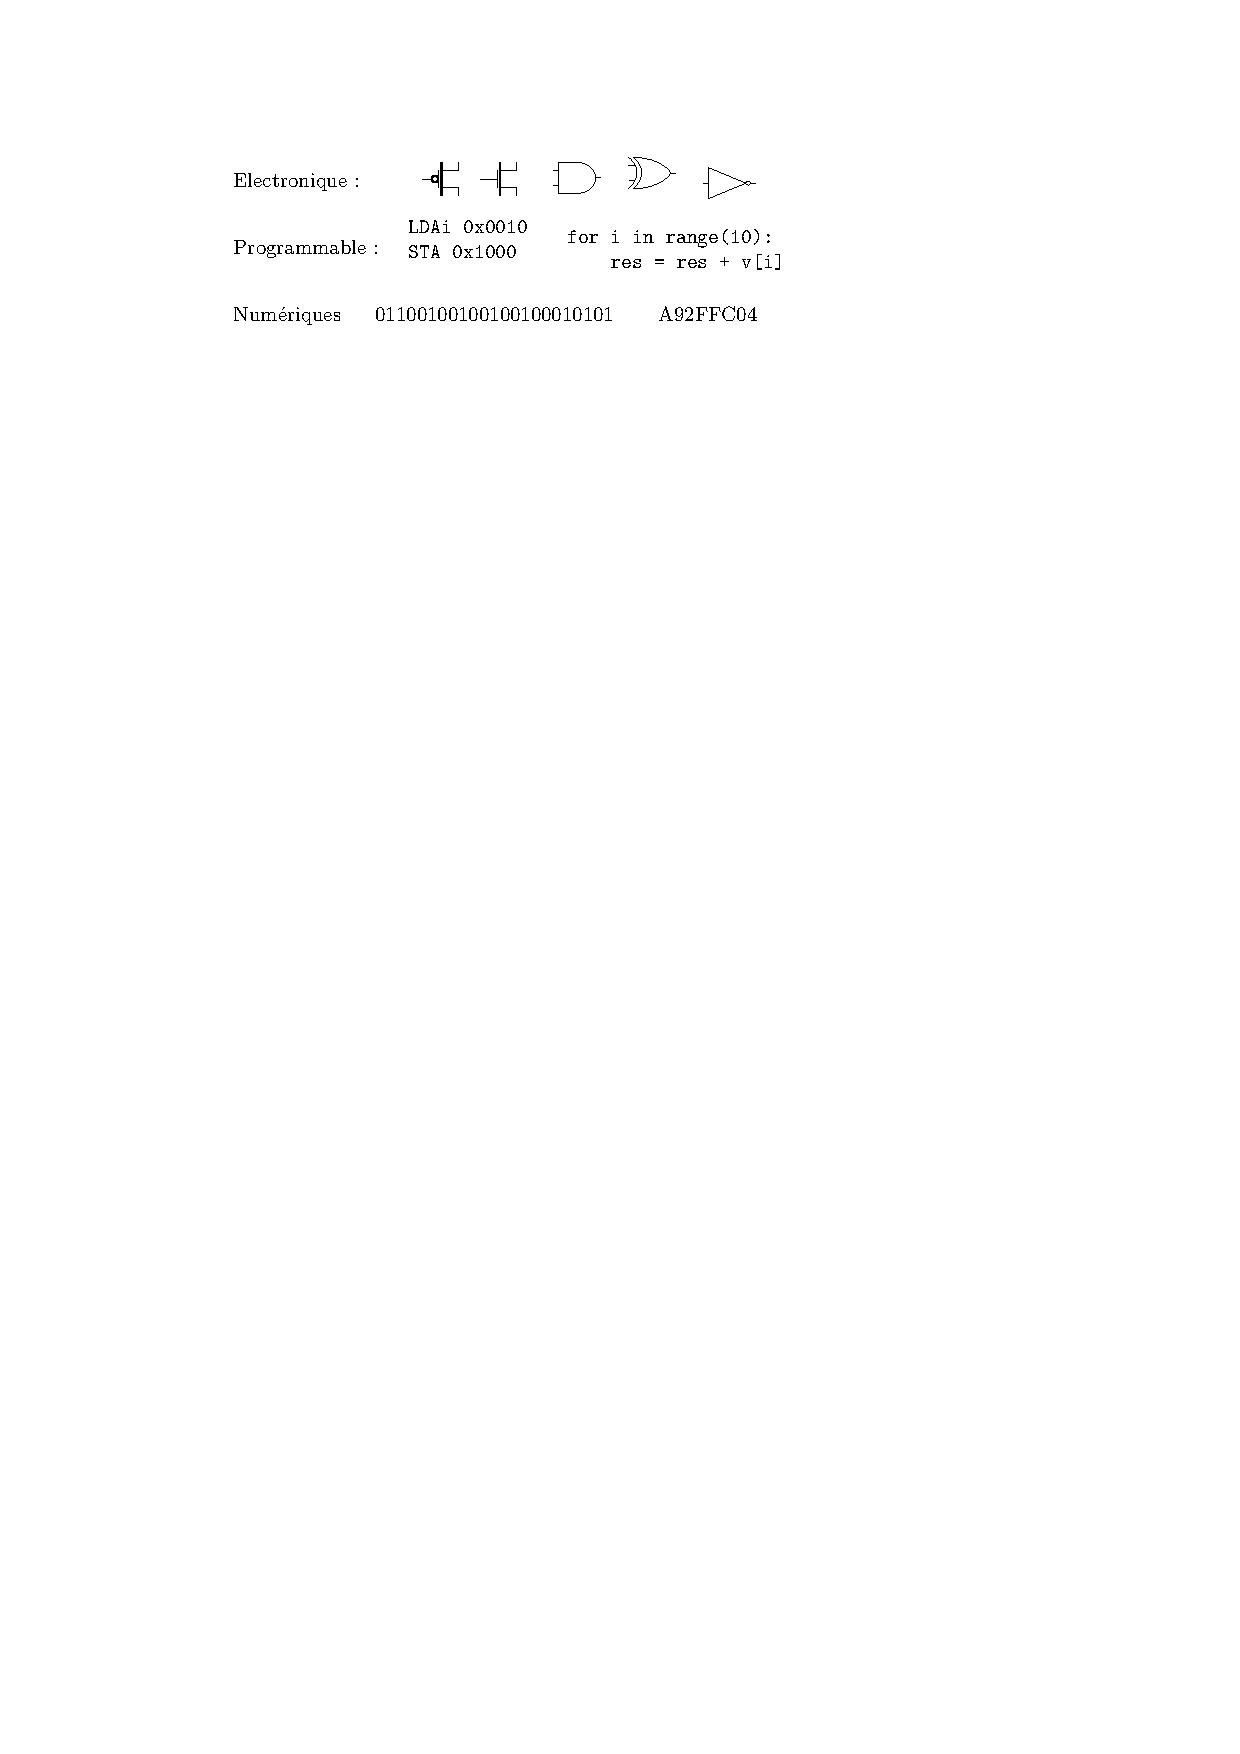
\includegraphics[width=\linewidth]{Figs/intro_elecprognum.pdf}
\end{frame}

\begin{frame}
\begin{block}{Particularités de ce cours}
\begin{itemize}
\item pas d'examen
\item les travaux de laboratoire ne sont pas notés
\item TD (1h30) regroupés en BE (3h), sur machine 
\end{itemize}
\end{block}
\begin{block}{Equipe pédagogique}
  \begin{tabular}{ccc}
    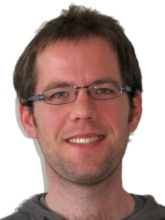
\includegraphics[width=0.1\columnwidth]{Figs/fix_jer.jpg}&
    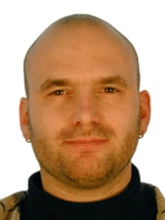
\includegraphics[width=0.1\columnwidth]{Figs/frezza.jpg}&
    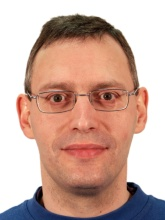
\includegraphics[width=0.1\columnwidth]{Figs/gutzwiller.jpg}\\
    J. Fix & H. Frezza-Buet & J.L. Gutzwiller
  \end{tabular}
  \end{block}
\end{frame}

\begin{frame}
  \begin{footnotesize}
  \begin{block}{Philosophie du cours}
    Introduire les concepts sous-jacents à n'importe quelle architecture sans être un cours sur une architecture spécifique (ARM, Intel, MIPS, ..)\\
    Abstraction progressive allant du bit à une architecture exécutant un jeu vidéo
  \end{block}
\begin{block}{Au programme}
\begin{itemize}
\item 4 x 1h30 $\Rightarrow$ représentations numériques, électronique, premier chemin de données, séquenceur
\item 1 BE (3h) et 1 TL (4h30)
\item 2 x 1h30 $\Rightarrow$ programmation
\item 1 BE (3h) : Programmation
\item 1 x 1h30 $\Rightarrow$ mémoires, périphériques et interruptions
\item 1 BE (3h) et 1 TL (4h30) : périphériques et ordonnanceur
\end{itemize}
\end{block}
\end{footnotesize}
\end{frame}

\begin{frame}
  On va introduire~:
  \begin{itemize}
  \item le codage binaire,
  \item les transistors ($\rightarrow$ ELAN - J. Maufoy)
  \item les systèmes logiques ($\rightarrow$ SLEA - Y. Houzelle)
  \item la programmation ($\rightarrow$ FISDA - F. Pennerath)
  \item les périphériques, interruptions
  \end{itemize}
  \begin{center}
    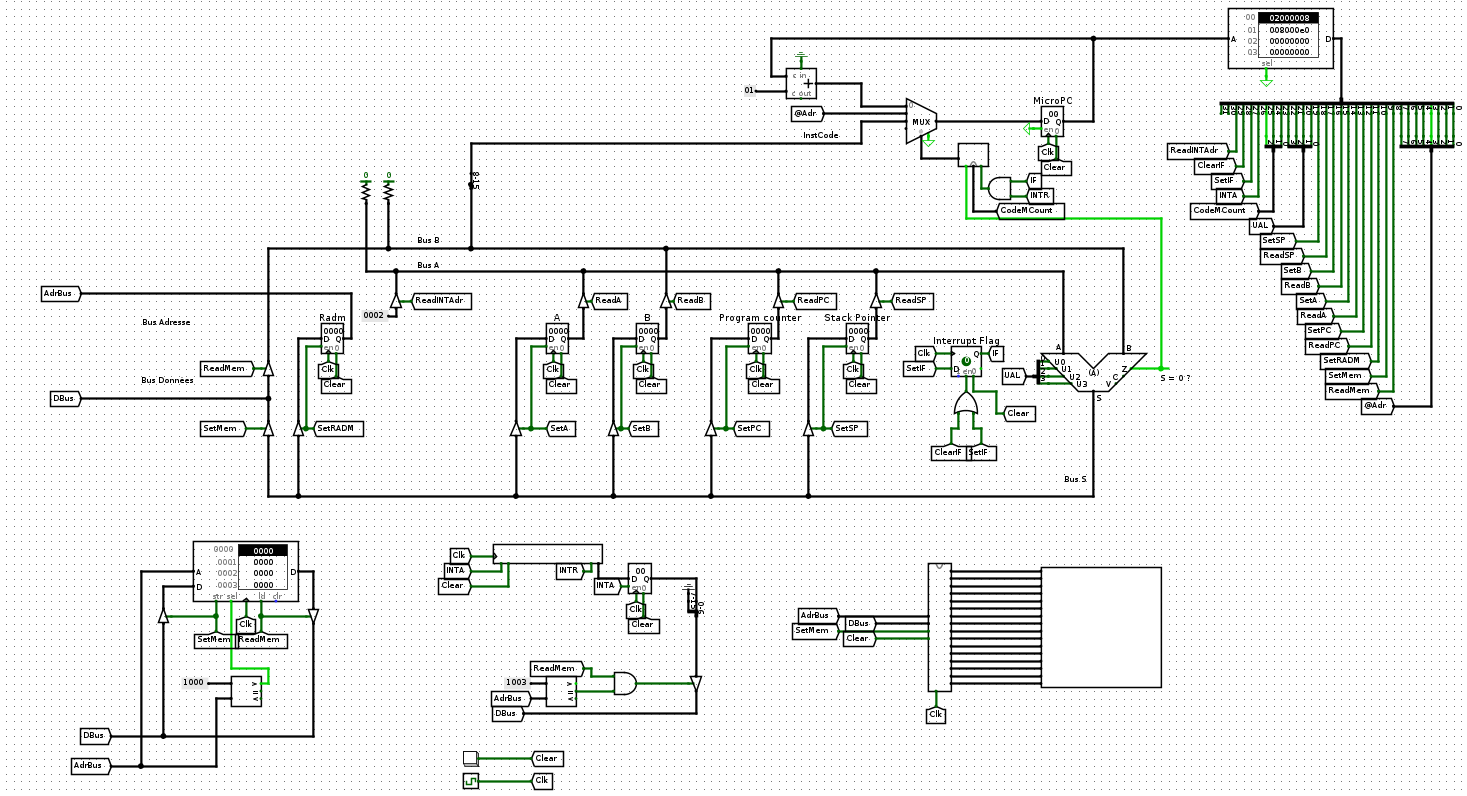
\includegraphics[width=0.7\columnwidth]{Figs/archi_jeu.png}
  \end{center}
\end{frame}

\begin{frame}
  \begin{center}\movie[width=8cm,height=4.5cm,showcontrols=true]{Space Invaders (1978)}{spaceinvaders.ogg}
    \end{center}
\end{frame}

%%%%%%%%%%%%%%%%%%%%%%%%%%%%
%%%%%%%%%%%%%%%%%%%%%%%%%%%%
\section{Codage et opérations binaires}

\begin{frame}
\begin{center}
\textbf{Codage et opérations binaires}
\end{center}
\end{frame}


%%%%%%%%%%%%%%%%%%%%%%%%%%%%
\subsection{Codage des entiers naturels}

\begin{frame}
\frametitle{Représenté et représentant}
Une valeur, quelle que soit sa nature, doit être représenté en binaire :\\
\begin{center}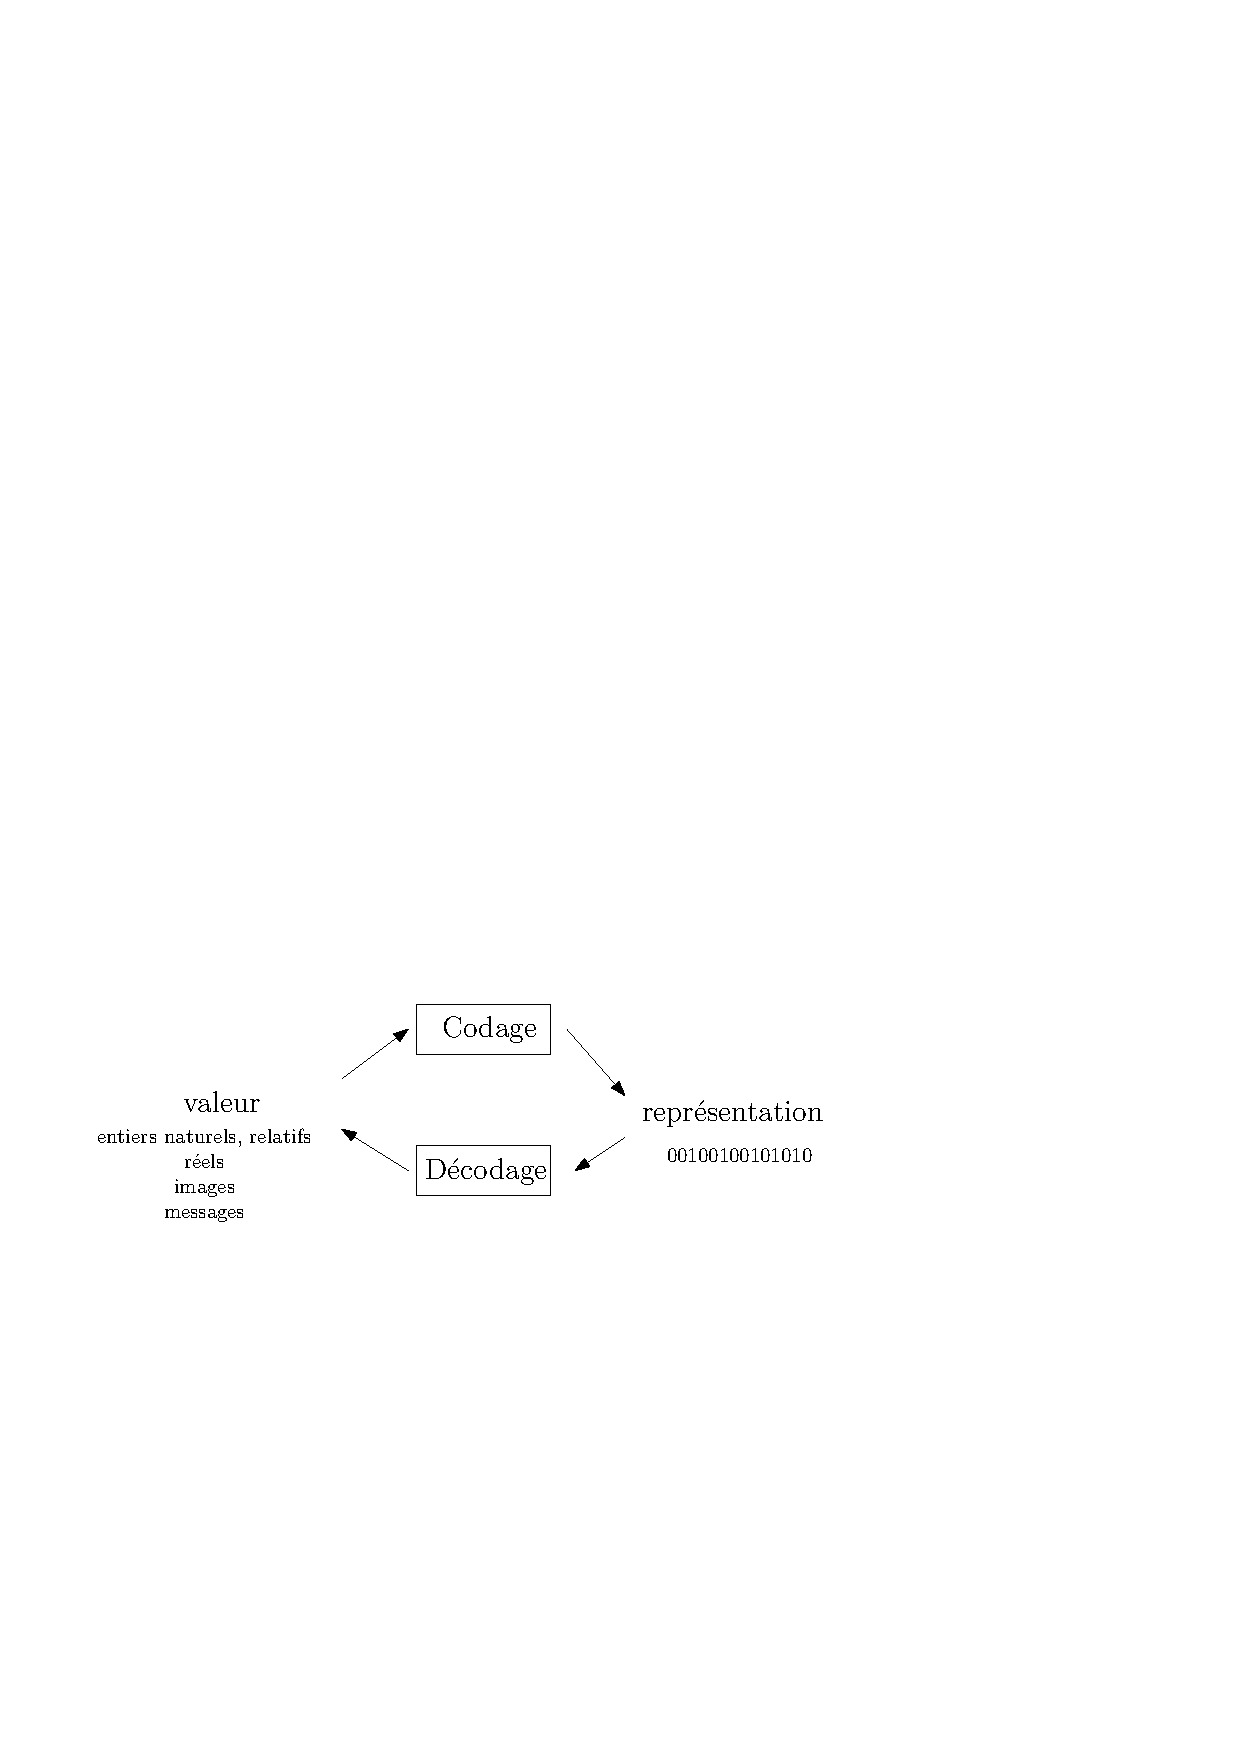
\includegraphics[width=0.75\linewidth]{Figs/codage_decodage.pdf}\end{center}
Bonne représentation ?
\begin{itemize}
\item facile à coder/décoder/manipuler, avec ou sans pertes
\item robuste aux perturbations, compact
\end{itemize}
\end{frame}

\begin{frame}
\frametitle{Représentation des entiers naturels}
\begin{figure}[htbp]
\begin{tabular}{ccc}

\includegraphics[width=0.25\linewidth]{Figs/Egypte/1527.pdf}&

\includegraphics[width=0.45\linewidth]{Figs/Mesopotamie/1527.pdf}&

\includegraphics[width=0.25\linewidth]{Figs/Shadock/dessin.pdf}\\
a) & b) & c)
\end{tabular}
\caption{a) Système additif des egyptiens, un symbole par puissance de 10; 1527; b) système mixte additif/positionnel des mésopotamiens en base 60 : $1527 = (20 + 5) * 60^1 + (20 + 7) * 60^0$; c) système positionnel des Shadoks : Bu-Zo-Ga-Mu $99 = 1.4^3 + 2.4^2 + 0.4 + 3$}
\end{figure}
\end{frame}

\begin{frame}
\frametitle{Représentation des entiers naturels}
En base 10 : 
\begin{eqnarray*}
34 = 3. 10^1 + 4. 10^0
\end{eqnarray*}
En base p : 
\begin{eqnarray*}
(a_{k-1}a_{k-2}\cdots a_{1}a_{0})_p = \sum_{i=0}^{k-1} a_i p^i
\end{eqnarray*}
avec $\forall i, a_i \in [0, p-1], a_{k-1} \neq 0$
\end{frame}

\begin{frame}
\frametitle{Représentation des entiers naturels}
Comment passer de la \textbf{représentation} base p à la \textbf{valeur} en base 10 ? 
\begin{eqnarray*}
(a_{k-1}a_{k-2}\cdots a_{1}a_{0})_p = \sum_{i=0}^{k-1} a_i p^i
\end{eqnarray*}
avec $\forall i, a_i \in [0, p-1], a_{k-1} \neq 0$. \\

Comment passer de \textbf{la valeur} $n$ en base 10 à \textbf{la représentation} en base p ? 
\begin{eqnarray*}
\sum_{i=0}^{k-1} a_i p^i = a_0 + p.(\sum_{0}^{k-2} a_{i+1} p^i)
\end{eqnarray*}
$\Rightarrow$ division euclidienne par $p$
\end{frame}

\begin{frame}
\frametitle{Représentation binaire, p=2 : $39 = 100111_2$}

\begin{eqnarray*}
\sum_{i=0}^{k-1} a_i p^i = a_0 + p.(\sum_{0}^{k-2} a_{i+1} p^i)
\end{eqnarray*}

\baseconversiontable{39}{2}\\
\begin{small}
\centering\begin{tabular}{c|c|c|c|c|c|c}
Puissance de 2 & $2^5 = 32$ & $2^4 = 16$ & $2^3= 8$ & $2^2=4$ & $2^1 = 2$ & $2^0 = 1$\\
\hline
$39_{10}$  &   1 &  0 & 0 & 1 & 1 &1 
\end{tabular}
\end{small}


\end{frame}

\begin{frame}
\frametitle{Représentation hexadécimale, p=16 : $39 = 27_{16}$}

\begin{center}\baseconversiontable{39}{16}\end{center}

Ou, à partir de la représentation binaire : 
\begin{eqnarray*}
39_{10} =  (\overbrace{0010}^{(2}\quad\overbrace{0111}^{7)})
\end{eqnarray*}

\end{frame}


\begin{frame}
\frametitle{Décimal codé binaire et code de gray}
Codage décimal codé binaire : 
\begin{eqnarray*}
421 = \overbrace{0100}^{4} \overbrace{0010}^{2} \overbrace{0001}^{1}
\end{eqnarray*}

Codage de Gray : 
\begin{center}
\begin{tabular}{c|c|c}
valeur & représentation binaire & représentation de Gray\\
\hline
0  & 000 & 000 \\
1  & 001 & 001 \\
2  & 010 & 011 \\
3  & 011 & 010 \\
4  & 100 & 110 \\
5  & 101 & 111 \\
6  & 110 & 101 \\
7  & 111 & 100
\end{tabular}
\end{center}

\end{frame}

%%%%%%%%%%%%%%%%%%%%%%%%%%%%
\subsection{Opérations arithmétiques sur les représentations non signées}

\begin{frame}
\frametitle{Addition}

Exemple : 001 + 011;

\begin{table}[h!]
\centering\begin{tabular}{cc}
\begin{tabular}{cc|cc}
$a$ & $b$ & Retenue & Reste\\
\hline
0 & 0 & 0 & 0\\
0 & 1 & 0 & 1\\
1 & 0 & 0 & 1\\
1 & 1 & 1 & 0
\end{tabular}&
\begin{tabular}{ccc|cc}
$a$ & $b$ & $r$& Retenue & Reste\\
\hline
0 & 0 & 0 & 0 & 0\\
0 & 1 & 0 & 0 & 1\\
1 & 0 & 0 & 0 & 1\\
1 & 1 & 0 & 1 & 0\\
0 & 0 & 1 & 0 & 1\\
0 & 1 & 1 & 1 & 0\\
1 & 0 & 1 & 1 & 0\\
1 & 1 & 1 & 1 & 1
\end{tabular}
\end{tabular}
\end{table}

\begin{itemize}
\item Algorithme d'addition de représentations non signées
\item Précision finie $\Rightarrow$ $n \in [0, 2^{k}-1]$ et bit de carry
\end{itemize}

\end{frame}

\begin{frame}
\frametitle{Autres opérations}
Soustraction : 
\begin{itemize}
\item a - b , a $\geq$ b
\item posée avec emprunt de retenue (e.g. $100_2 - 001_2$)
\end{itemize}
Multiplication :
\begin{itemize}
\item addition et décalage (e.g. $39 \times 5$)
\end{itemize}
Division : 
\begin{itemize}
\item posée  (e.g. $39 / 5$)
\end{itemize}

Entiers négatifs ?!

\end{frame}

\begin{frame}
\frametitle{Représentation des entiers relatifs}
\begin{small}
\begin{block}{Codage par décalage (excess-K)}
\begin{itemize}
\item $n \in [-2^{k-1}, 2^{k-1}-1]$, $K = 2^{k-1}$
\item Codage : $x = EncUB_k(n + K)$, $n+K \in [0, 2^k -1]$
\item Décodage : $n = DecUB(x) - K = \sum_{i=0}^{k-1} x_i 2^i - 2^{k-1}$
  \begin{center}
\begin{tabular}{c|c|c|c|c|c|c|c|c}
$n$ & -4 & -3 & -2& -1 & 0 & 1 & 2 & 3\\
\hline
$x$ & $000_{2K}$ & $001_{2K}$ & $010_{2K}$ & $011_{2K}$ & $100_{2K}$ & $101_{2K}$ & $110_{2K}$ & $111_{2K}$
\end{tabular}
\end{center}
\item addition particulière (-4 + 1, k=3). comparaison facile.
\end{itemize}
\end{block}
\end{small}
\end{frame}

\begin{frame}
  \frametitle{Représentation des entiers relatifs}
  \begin{small}
\begin{block}{Codage par valeur signée (sign-magnitude)}
\begin{itemize}
\item $n \in [-2^{k-1}+1, 2^{k-1}-1]$
\item un bit de signe, k-1 bits de valeur
 \begin{center}
\begin{tabular}{c|c|c|c|c|c|c|c|c}
$n$ & -3 & -2& -1 & 0 & 1 & 2 & 3 \\
\hline
$x$ & $111_{2s}$ & $110_{2s}$ & $101_{2s}$ & $100_{2s}$\mbox{ ou } $000_{2s}$ & $001_{2s}$ & $010_{2s}$ & $011_{2s}$
\end{tabular}
\end{center} 
\item 2 représentations de 0. Addition particulière(1 + (-1), k=3).
\end{itemize}
\end{block}
\end{small}
\end{frame}

\begin{frame}
\frametitle{Représentation des entiers relatifs}
\begin{block}{Codage par complément à deux (2's complement)}
\begin{itemize}
\item $n \in [-2^{k-1}, 2^{k-1}-1]$
  \begin{center}
\begin{tabular}{c|c|c|c|c|c|c|c|c|c}
$n$ & -4 & -3 & -2& -1 & 0 & 1 & 2 & 3 \\
\hline
1C & (011) & 100 & 101 & 110 & 111 ou 000 & 001 & 010 & 011\\
\hline
2C & 100 & 101 & 110 & 111 & 000 & 001 & 010 & 011
\end{tabular}
\end{center}
\item les opérations sont les mêmes qu'avec les représentations non signées
\item comparaison : 1) tester le signe 2) sinon la valeur
\item une seule représentation du 0
\item débordement (\emph{overflow}); e.g. k=3 :  3 + 3 ; (-3) + (-3), vérifiable avec les bits de retenue (01 ou 10)
\end{itemize}
\end{block}
\end{frame}

\begin{frame}
\frametitle{Représentation des nombres réels}
\begin{block}{Virgule fixe (fixed-point)}
\begin{itemize}
\item $26.5 = 2 \times 10^1 + 6 \times 10^0 + 5 \times 10^{-1}$
\item Codage du ``.'' ? $26.5 = 11010.1_2$; Convention $Q<n_e><n_f>$
\item Codage : représentation non signée de $n \times 2^{n_f}$
\item Décodage : $n = \sum_{i=0}^{k-1} a_i 2^{i - n_f} = 2^{-n_f} \sum_{i=0}^{k-1} a_i 2^i$
\item complément à deux (e.g. $5.25 - 3.5$ ; $-5.25 + 3.5$ en Q4.2)
\item même opérations arithmétiques que pour les entiers (DSP)
\item mais précision uniforme, non représentation de valeurs particulières (e.g. $\infty, NaN$, ..)
\end{itemize}
\end{block}
\end{frame}


\begin{frame}
\frametitle{Représentation des nombres réels}
\begin{block}{Virgule flottante IEEE 754-2008 (floating-point)}
\begin{itemize}
\item Notation scientifique en base p :\\
 $x = \pm m \times p^{e}$, $m \in [0, p[, e \in \mathbb{Z}$
\item $1245 = 1.245 \times 10^3 = 0.1245 \times 10^4 = 0.01245 \times 10^5$
\item représentation\underline{\textbf{s}} dénormalis\underline{\textbf{ées}} ($m = 0$); représentation normalisée ($m \neq 0$)
\item En binaire , $m \in [0, 2[$; {\'E}tendu $\mathbb{R} \cup \{-\infty, \infty\} \cup \{\mbox{sNan}, \mbox{qNan}\}$
\end{itemize}
\begin{center}\begin{tabular}{|c|c|c|}
\hline
signe S (1 bit)& exposant E ($n_e$ bits)& mantisse M ($n_m$ bits)\\
\hline
\end{tabular}
\end{center}
M code uniquement la partie fractionnaire. E en excess-K.\\
Plusieurs conventions : binary-16, binary-32, binary-64
\end{block}
\end{frame}

\begin{frame}
  \frametitle{Représentation des nombres réels}
  \begin{block}{Binary-16}
    Représentation sur 16 bits :1 bit de signe,$n_e = 5$ bits pour l'exposant, $n_m=10$ bits pour la mantisse
    \begin{footnotesize}
    \begin{center}
\begin{tabular}{ccc|c|c}
\multicolumn{3}{c}{Représentation binary-16} & Valeur représentée & Note\\
Signe & Exposant & Mantisse & & \\
\hline\hline
0&00000&0$\cdots$0 & +0 & \\
1&00000&0$\cdots$0 & -0 & \\
s&00000&0$\cdots$01 & $(-1)^s 2^{-14} 1.2^{-10} = (-1)^s 2^{-24}$ & Plus petit réél dénormalisé\\
s&00000&0$\cdots$10 & $(-1)^s 2^{-14} 2.2^{-10} = (-1)^s 2^{-23}$ & Second plus petit réel\\
s&00000&1$\cdots$11 & $(-1)^s (2^{-14} - 2^{-24})$ & Plus grand réel dénormalisé\\
s&00001&0$\cdots$00 & $(-1)^s 2^{1-15} = (-1)^s 2^{-14}$ & Plus petit réel normalisé \\
s&11110&1$\cdots$11 & $(-1)^s 2^{15} (2 - 2^{-10})$& Plus grand réel normalisé \\
s&11111&0$\cdots$00 & $(-1)^s \infty$ & \\
x&11111& M, $M \neq 0$ & NaN (sNan ou qNan) & Exception, e.g 0/0, ..
\end{tabular}
    \end{center}
    \end{footnotesize}
  \end{block}
\end{frame}


\begin{frame}
\frametitle{Représentation des caractères (ASCII, ISO-8859, UTF-8)}
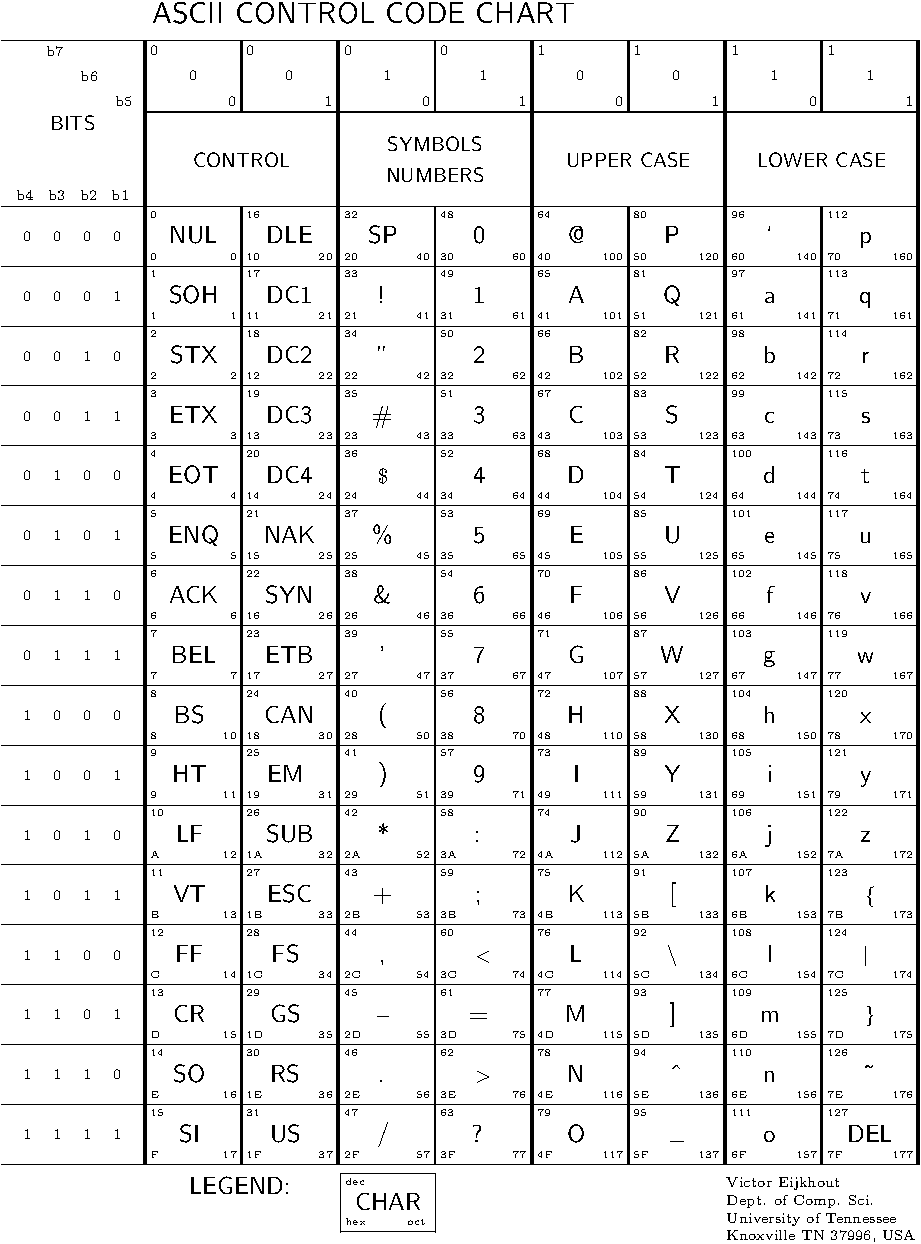
\includegraphics[width=0.35\linewidth]{Figs/ascii_table.pdf}
Norme trop spécifique à l'Américain. Multiplicité des normes ISO-8859-x sur 8 bits; Norme UTF-8

\end{frame}

\begin{frame}
\frametitle{Devinette}
\uncover<1->{
\begin{center}
Quelle est la valeur de $(626F6E6A6F757221)_{16}$ ?
\end{center}}

\begin{enumerate}
	\item<2-> ``bonjour!'' en ASCII
	\item<3-> 7 093 009 341 547 377 185 , entier non signé sur 64 bits
        \item<4-> 
\includegraphics[width=0.3\linewidth]{Figs/code_img.pdf}, un octet code un niveau de gris (0:noir, 255:blanc)
\end{enumerate}
\end{frame}


%%%%%%%%%%%%%%%%%%%%%%%%%%%%
%%%%%%%%%%%%%%%%%%%%%%%%%%%%
\section{La couche physique}

\begin{frame}
\begin{center}
\textbf{La couche physique et la couche logique}
\end{center}
\end{frame}

\subsection{Le bit}
\begin{frame}
  \frametitle{Représentation physique et manipulation d'un bit}
  \begin{block}{Représentation}
    Un bit (0, 1) va être représenté physiquement par un niveau de tension\\
    Par une valeur ? Par des domaines contigus ? Séparés par des marges ?\\
  \end{block}
  \begin{block}{Manipulation}
    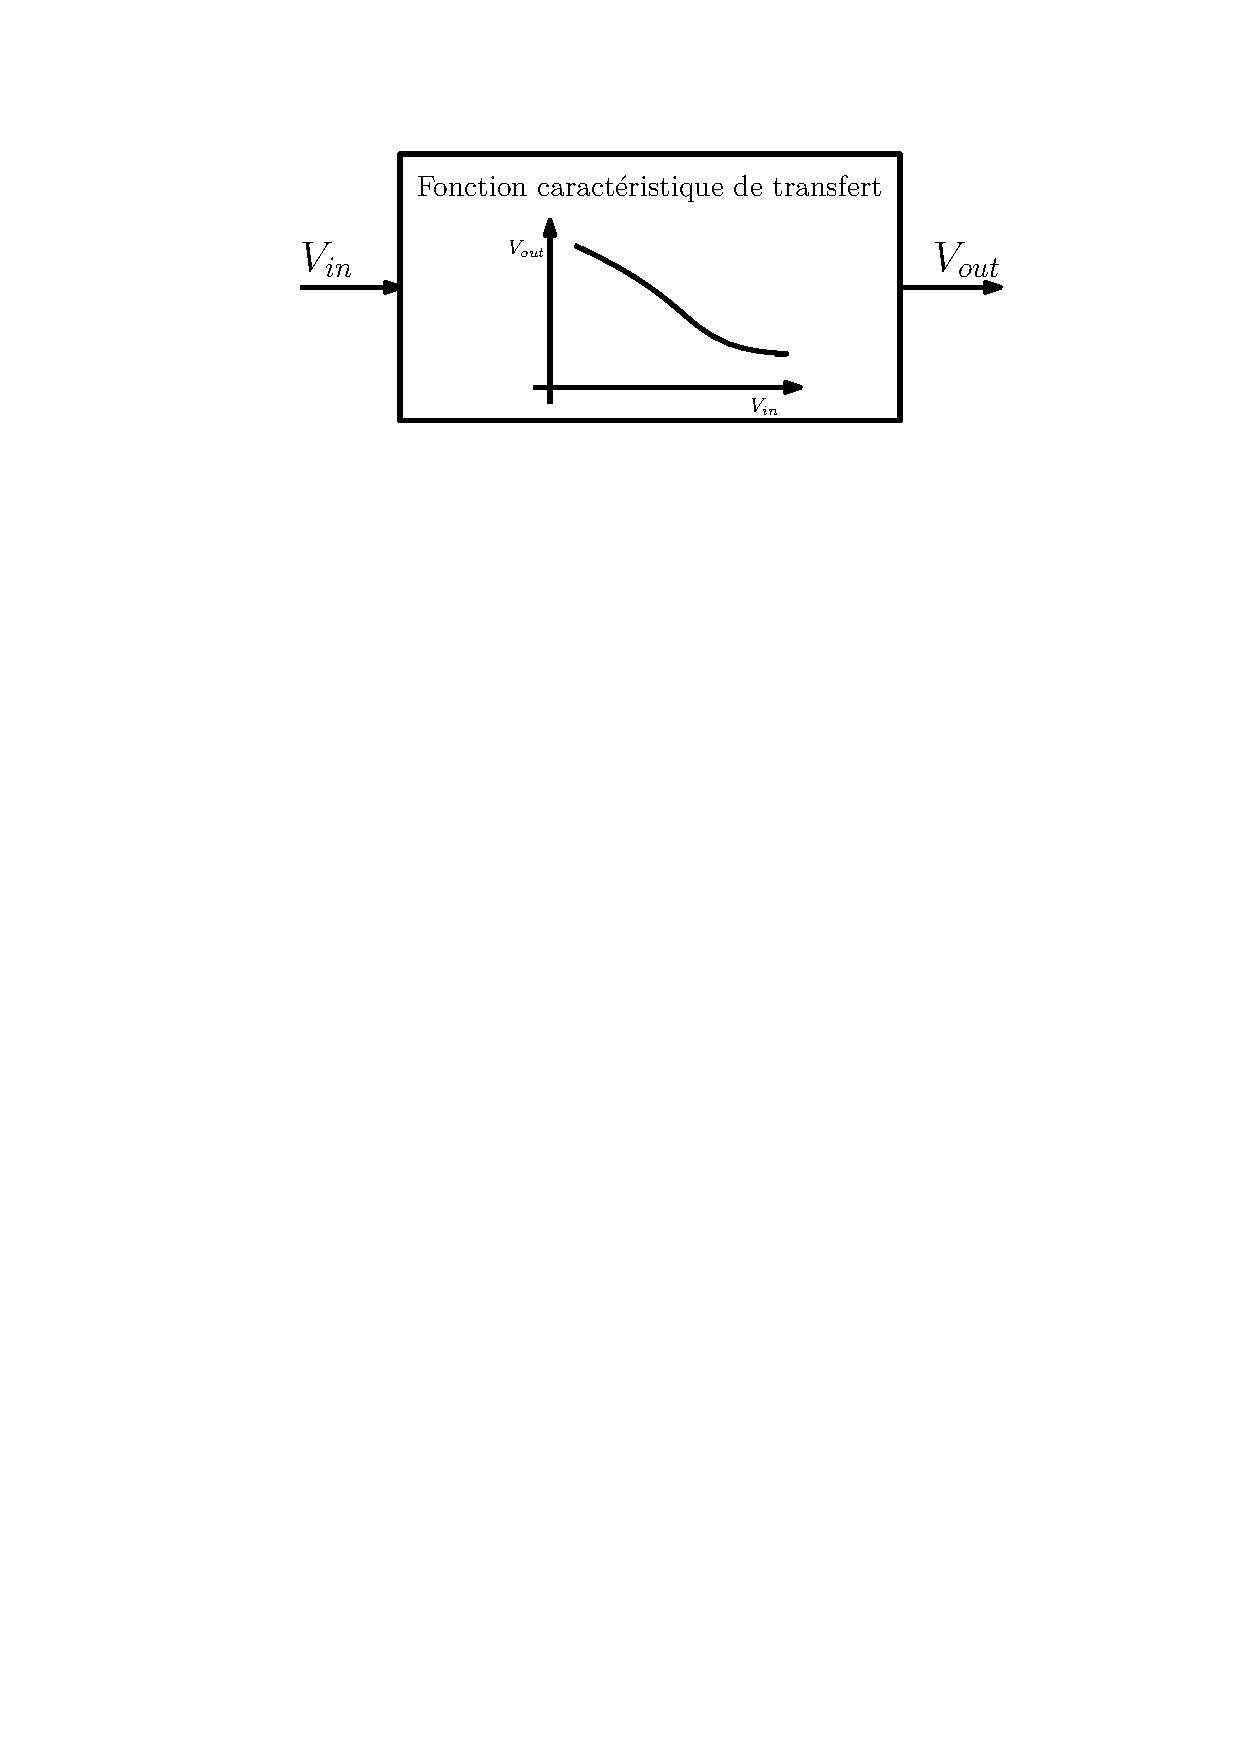
\includegraphics[width=0.3\columnwidth]{Figs/vtc.pdf}\hfill
    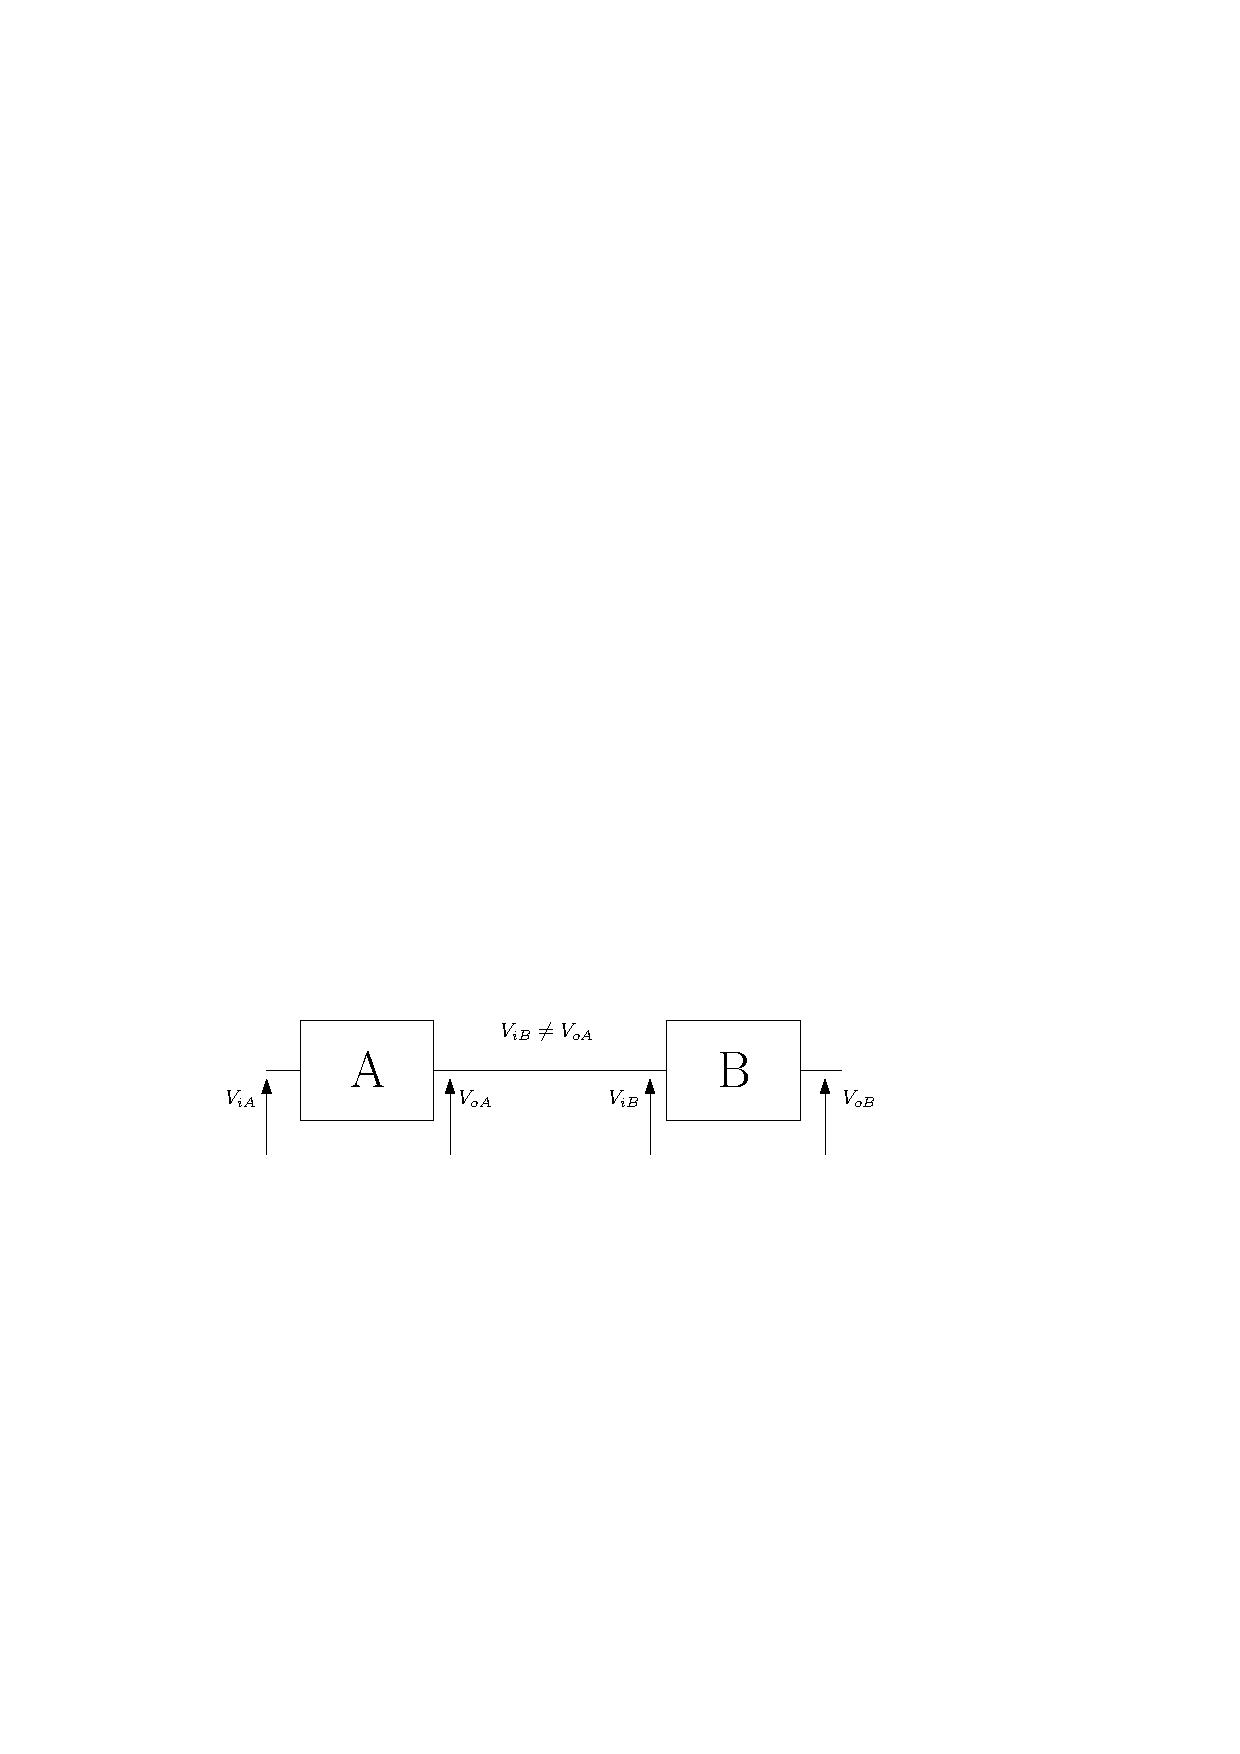
\includegraphics[width=0.4\columnwidth]{Figs/VTC_connect.pdf}\\
    Des marges différentes en entrée et en sortie.\\
    Il nous faut un composant avec une VTC non linéaire
    \end{block}
\end{frame}

\begin{frame}
  \frametitle{Au début, le relais}
  \begin{figure}[htbp]
    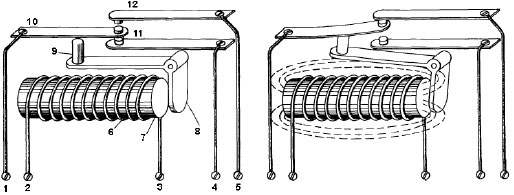
\includegraphics[width=0.8\columnwidth]{Figs/relay.jpg}
    \caption{Relais électromécanique de J. Henry (1930-1940)}
  \end{figure}
\end{frame}

\subsection{Le transistor}

\begin{frame}
  \frametitle{Puis vient le transistor (1947)}
\begin{figure}
\begin{center}
\begin{tabular}{cccc}
\begin{circuitikz}[scale = 0.8, transform shape]
\draw	(0,0) node[npn](npn1){};
\node at ($(npn1.B) - (0.5,0)$) {Base};
\node at ($(npn1.E) - (0, 0.5)$) {Emetteur};
\node at ($(npn1.C) + (0, 0.5)$) {Collecteur};
\end{circuitikz} &
\begin{circuitikz}
\draw	(0,0) node[pnp](pnp1){};
\node at ($(pnp1.B) - (0.5,0)$) {Base};
\node at ($(pnp1.E) + (0, 0.5)$) {Emetteur};
\node at ($(pnp1.C) - (0, 0.5)$) {Collecteur};
\end{circuitikz} &
\begin{circuitikz}
\draw (0, 0) node[nmos] (nmos1) {};
\node at ($(nmos1.gate) - (0.5,0)$) {Grille};
\node at ($(nmos1.drain) + (0, 0.5)$) {Drain};
\node at ($(nmos1.source) - (0, 0.5)$) {Source};
\end{circuitikz} &
\begin{circuitikz}
\draw (0, 0) node[pmos] (pmos1) {};
\node at ($(pmos1.gate) - (0.5,0)$) {Grille};
\node at ($(pmos1.drain) - (0, 0.5)$) {Drain};
\node at ($(pmos1.source) + (0, 0.5)$) {Source};
\end{circuitikz} \\
a) & b) & c) & d)
\end{tabular}
\end{center}
\caption{\label{fig:transistor_bipolaire} a) Transistor bipolaire NPN. b) Transistor bipilaire PNP. c) Transistor unipolaire NMOS. d) Transistor unipolaire PMOS}
\end{figure}
\end{frame}

\begin{frame}
  \frametitle{Un interrupteur commandable}
  \begin{block}{TTL, CMOS et circuits}
   \begin{minipage}[c]{.56\linewidth}
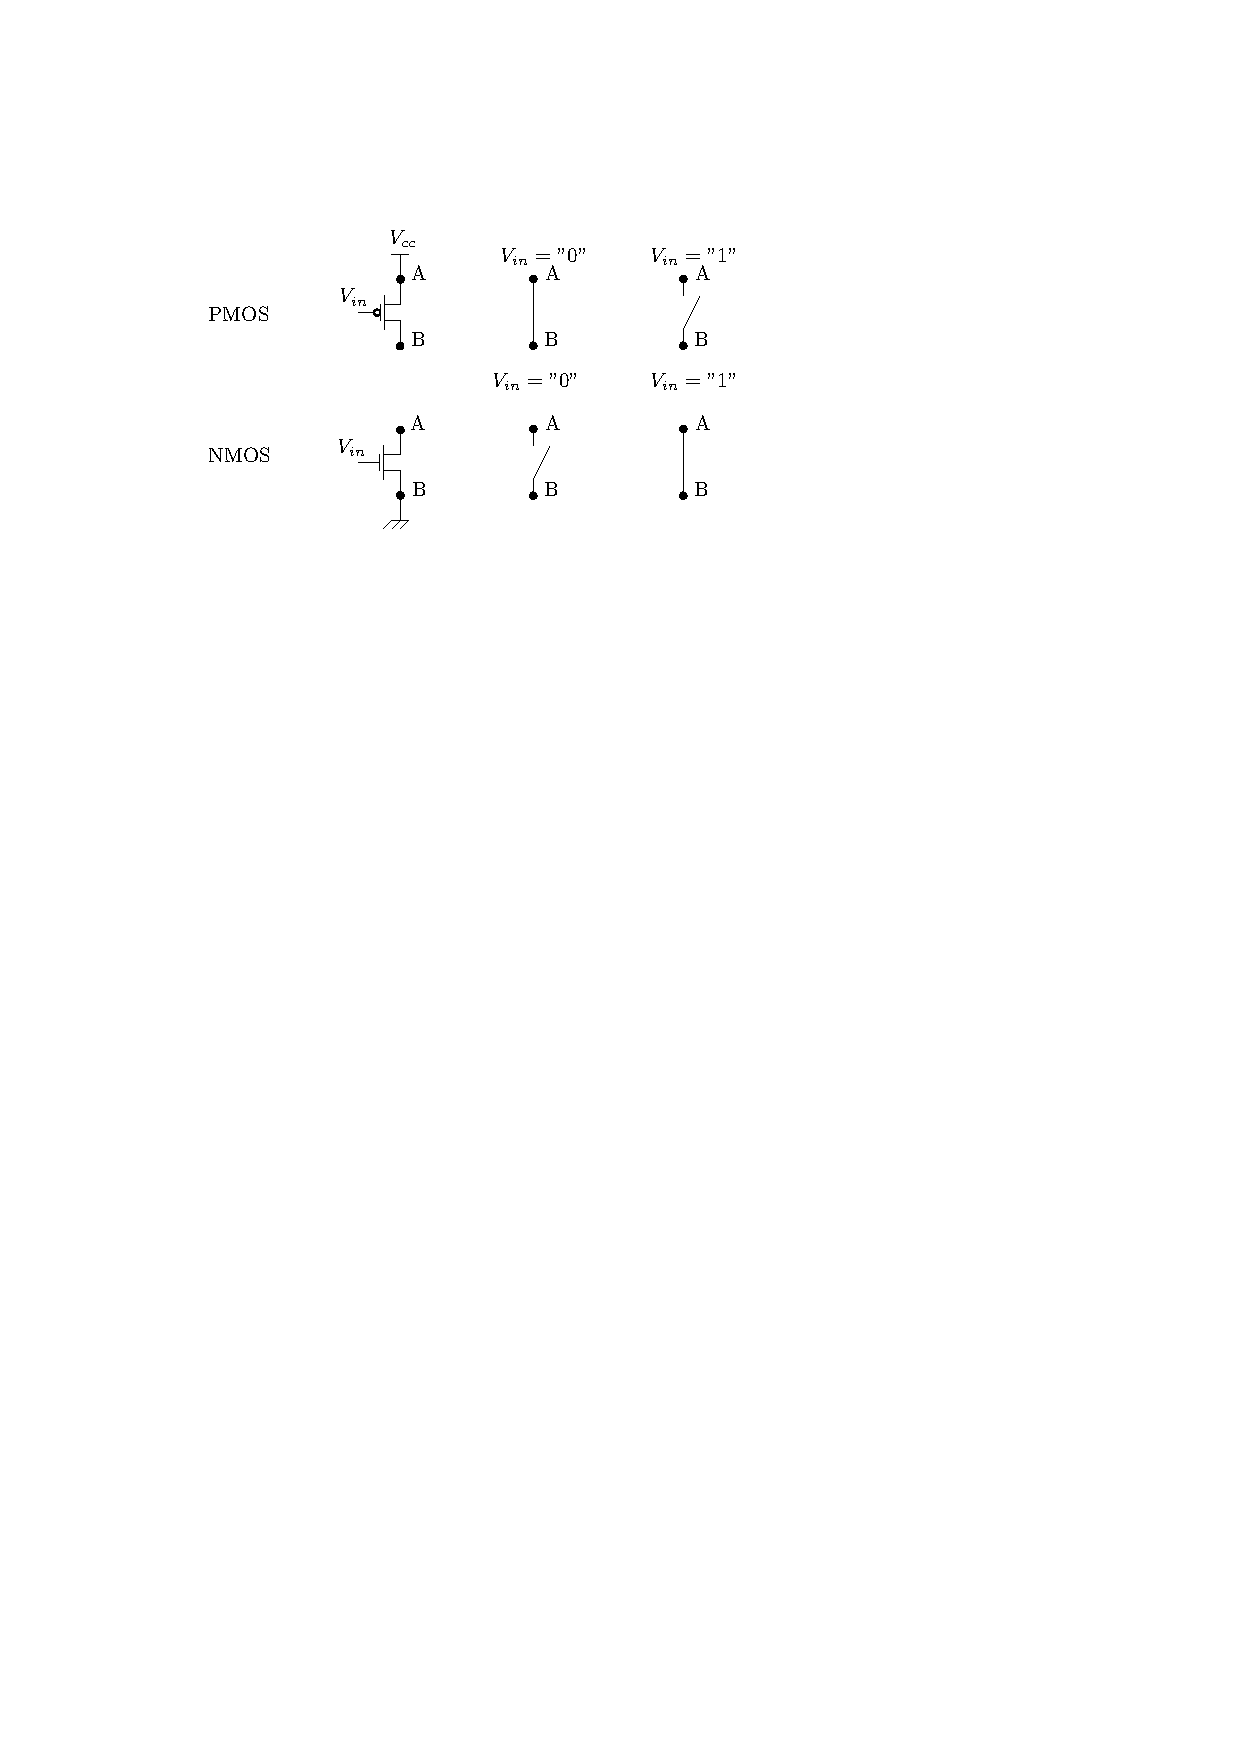
\includegraphics[width=\columnwidth]{Figs/nmospmos.pdf} \\\centering a)
   \end{minipage} \hfill
   \begin{minipage}[c]{.25\linewidth}
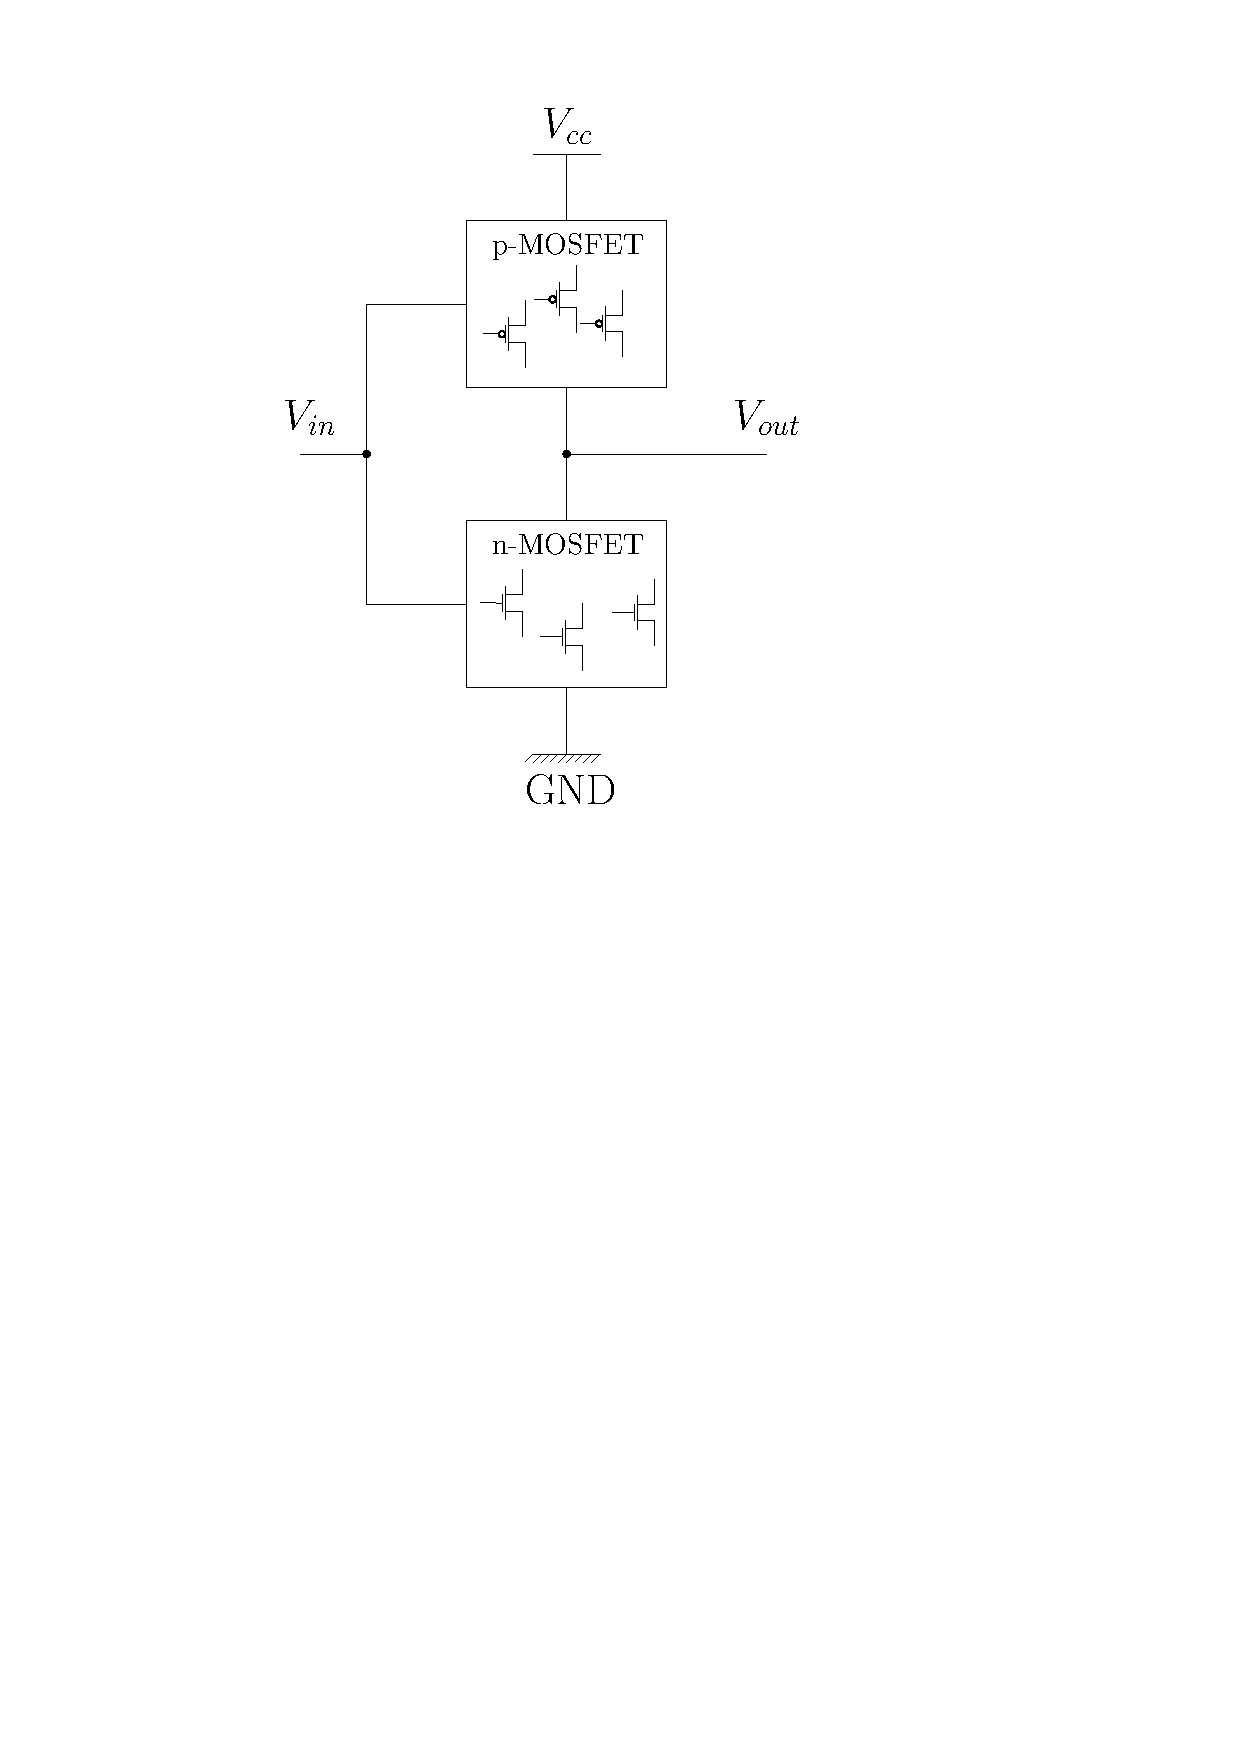
\includegraphics[width=\columnwidth]{Figs/circuits_mos.pdf}\\\centering b)
   \end{minipage}
\end{block}
\end{frame}

\subsection{Circuits de transistors}

\begin{frame}
  \frametitle{Notre premier circuit}
  \begin{block}{Inverseur (\emph{Not}) : $S=\overline{A}$}

\begin{figure}[htbp]
   \begin{minipage}[c]{.25\linewidth}
\begin{circuitikz}[scale=0.7, every node/.style={scale=0.7}]
\draw[color=black, thick]
        (0,1.0) node[nmos](nmos1){}
        (0,3.0) node[pmos](pmos1){}

        (nmos1.gate) -- (pmos1.gate) node[midway] (Vin) {}
        (nmos1.drain) -- (pmos1.drain) node[midway] (Vout){} 
        (pmos1.source) to [short,-o](0,4.5) node[right]{$V_{cc}$}
        (nmos1.source) to [short](0,0.5) node[ground]{}
        (Vout) to ($(Vout) + (1.0,0)$) node[right, short] {$V_{S}$}
        (nmos1.gate) -| (Vin) to ($(Vin) + (-1.0,0)$) node[left, short] {$V_{A}$};
\end{circuitikz}\\\centering a)
   \end{minipage}\hspace{2cm}
   \begin{minipage}[c]{.25\linewidth}
\tikzstyle{branch}=[fill,shape=circle,minimum size=3pt,inner sep=0pt]
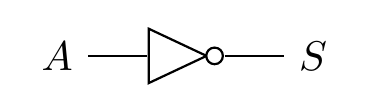
\begin{tikzpicture}[thick,scale=1.5, every node/.style={scale=1.5}]
\draw[color=black,thick]
     (0,0) node[not gate US, draw, logic gate inputs=nn] (Not1) {}
     (Not1.input) -- ($(Not1.input) - (0.5,0)$) node[left] {$A$}
     (Not1.output) -- ($(Not1.output) + (0.5, 0)$) node[right] {$S$};
\end{tikzpicture}\\\centering b)
   \end{minipage}
\caption{\underline{\textbf{Une}} réalisation possible d'une porte NOT en technologie CMOS. b) Symbole normalisé (norme Américaine).}
\end{figure}
  \end{block}
\end{frame}

\begin{frame}
  \frametitle{Circuits à deux entrées}
  \begin{block}{Porte NAND : $S = \overline{A.B}$}

  \begin{figure}[htbp]
   \begin{minipage}[c]{.46\linewidth}
\begin{circuitikz}[scale=0.6, every node/.style={scale=0.6}]
\draw[color=black, thick]
        (0,3.0) node[nmos](nmos1){}
        (0,5.0) node[pmos](pmos1){}
        (0,1.5) node[nmos](nmos2){}
        (2.0,5.0) node[pmos,xscale=-1](pmos2){}

        (nmos1.gate) -- ($(nmos1.gate) - (0.2,0)$) node[left] {$V_A$}
        (pmos1.gate) -- ($(pmos1.gate) - (0.2,0)$) node[left] {$V_A$}
        (nmos2.gate) -- ($(nmos2.gate) - (0.2,0)$) node[left] {$V_B$}
        (pmos2.gate) -- ($(pmos2.gate) + (0.2,0)$) node[right] {$V_B$}
        (pmos1.drain) -- (nmos1.drain)
        (pmos2.drain) -- (pmos1.drain)
        (pmos1.source) -- (pmos2.source) node[midway] (Vcc) {}
        (Vcc) to [short,-o] ($(Vcc) + (0,0.2)$) node[above] {$V_{cc}$}
        (nmos1.drain) -- ($(nmos1.drain) + (1.0, 0)$) node[right] {$V_S$}
        (nmos2.source) -- ($(nmos2.source) + (0, -0.1)$) node[ground]{};
\end{circuitikz}\\\centering a)
   \end{minipage} \hfill
   \begin{minipage}[c]{.46\linewidth}
\tikzstyle{branch}=[fill,shape=circle,minimum size=3pt,inner sep=0pt]
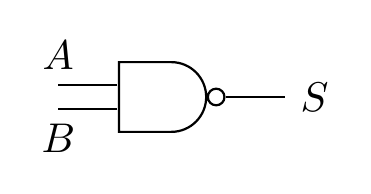
\begin{tikzpicture}[thick,scale=1.5, every node/.style={scale=1.5}]
\draw[color=black,thick]
     (0,0) node[nand gate US, draw, logic gate inputs=nn] (Nand1) {}
     (Nand1.input 1) -- ($(Nand1.input 1) - (0.5,0)$) node[left,above] {$A$}
     (Nand1.input 2) -- ($(Nand1.input 2) - (0.5,0)$) node[left,below] {$B$}
     (Nand1.output) -- ($(Nand1.output) + (0.5, 0)$) node[right] {$S$};
\end{tikzpicture}\\\centering b)
   \end{minipage}
\caption{\label{fig:nand_cmos} a) \underline{\textbf{Une}} réalisation possible d'une porte NAND en technologie CMOS. b) Symbole normalisé}
\end{figure}  
    \end{block}
\end{frame}

\begin{frame}
  \frametitle{Circuits à deux entrées}
  \begin{block}{Porte NOR : $S = \overline{A+B}$}
\begin{figure}[htbp]
   \begin{minipage}[c]{.46\linewidth}
\begin{circuitikz}[scale=0.6, every node/.style={scale=0.6}]
\draw[color=black, thick]
        (0.0,5.0) node[pmos](pmos2){}
        (0,3.5) node[pmos](pmos1){}
        (0,1.5) node[nmos](nmos1){}
        (2.0,1.5) node[nmos,xscale=-1](nmos2){}

        (nmos1.gate) -- ($(nmos1.gate) - (0.2,0)$) node[left] {$V_A$}
        (pmos1.gate) -- ($(pmos1.gate) - (0.2,0)$) node[left] {$V_A$}
        (nmos2.gate) -- ($(nmos2.gate) + (0.2,0)$) node[right] {$V_B$}
        (pmos2.gate) -- ($(pmos2.gate) - (0.2,0)$) node[left] {$V_B$}

        (nmos1.source) -- (nmos2.source) node[midway] (gnd) {}
        (gnd) -- ($(gnd) + (0, -0.1)$) node[ground]{}
        (pmos2.source) to [short,-o] ($(pmos2.source) + (0, 0.2)$) node[above] {$V_{cc}$}
        (nmos1.drain) -- (nmos2.drain)
        (pmos1.drain) -- (nmos1.drain) node[midway] (Vs) {}
        (pmos1.drain) -- ($(pmos1.drain) + (2.0, 0)$) node[right] {$V_S$};
\end{circuitikz}\\\centering a)
   \end{minipage} \hfill
   \begin{minipage}[c]{.46\linewidth}
\tikzstyle{branch}=[fill,shape=circle,minimum size=3pt,inner sep=0pt]
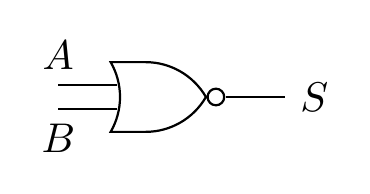
\begin{tikzpicture}[thick,scale=1.5, every node/.style={scale=1.5}]
\draw[color=black,thick]
     (0,0) node[nor gate US, draw, logic gate inputs=nn] (Nor1) {}
     (Nor1.input 1) -- ($(Nor1.input 1) - (0.5,0)$) node[left,above] {$A$}
     (Nor1.input 2) -- ($(Nor1.input 2) - (0.5,0)$) node[left,below] {$B$}
     (Nor1.output) -- ($(Nor1.output) + (0.5, 0)$) node[right] {$S$};
\end{tikzpicture}\\\centering b)
   \end{minipage}
\caption{\label{fig:nor_cmos} a) \underline{\textbf{Une}} réalisation possible d'une porte NOR en technologie CMOS. b) Symbole normalisé.}
\end{figure}
    \end{block}
\end{frame}

\begin{frame}
  \frametitle{Circuits à deux entrées}
  \begin{block}{On essaye une AND : $S = A.B$}
    
\only<2-5>{
\begin{circuitikz}[scale=0.6, transform shape]
\draw[color=black, thick]
        (0,3.0) node[pmos](pmos1){}
        (0,5.0) node[nmos](nmos1){}
        (0,1.5) node[pmos](pmos2){}
        (2.0,5.0) node[nmos,xscale=-1](nmos2){}

        (pmos1.gate) -- ($(pmos1.gate) - (0.2,0)$) node[left] {$V_A$}
        (nmos1.gate) -- ($(nmos1.gate) - (0.2,0)$) node[left] {$V_A$}
        (pmos2.gate) -- ($(pmos2.gate) - (0.2,0)$) node[left] {$V_B$}
        (nmos2.gate) -- ($(nmos2.gate) + (0.2,0)$) node[right] {$V_B$}
        (nmos1.source) -- (pmos1.source)
        (nmos2.source) -- (nmos1.source)
        (nmos1.drain) -- (nmos2.drain) node[midway] (Vcc) {}
        (Vcc) to [short,-o] ($(Vcc) + (0,0.2)$) node[above] {$V_{cc}$}
        (pmos1.source) -- ($(pmos1.source) + (1.0, 0)$) node[right] {$V_S$}
        (pmos2.drain) -- ($(pmos2.drain) + (0, -0.1)$) node[ground]{};
\onslide<3->{\draw[red, very thick] (-1,1) -- (4,6) node [midway, above, sloped] {INTERDIT};}
\end{circuitikz}
}
\only<4-5>{
  \onslide<4>{On fait comment ??}
  \onslide<5->{
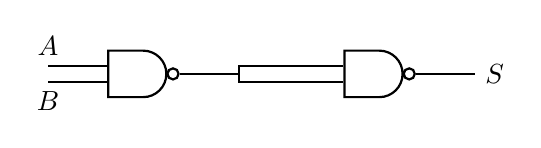
\begin{tikzpicture}[thick,scale=1.5, every node/.style={scale=1.}]
\draw[color=black,thick]
     (0,0) node[nand gate US, draw, logic gate inputs=nn] (Nand1) {}
     (2.,0) node[nand gate US, draw, logic gate inputs=nn] (Nand2) {}
     (Nand1.input 1) -- ($(Nand1.input 1) - (0.5,0)$) node[left,above] {$A$}
     (Nand1.input 2) -- ($(Nand1.input 2) - (0.5,0)$) node[left,below] {$B$}
     (Nand1.output) -- ++(right:5mm) |- (Nand2.input 1)
     (Nand1.output) -- ++(right:5mm) |- (Nand2.input 2)
     (Nand2.output) -- ($(Nand2.output) + (0.5, 0)$) node[right] {$S$};
\end{tikzpicture}\\
    }
  }
    \end{block}
\end{frame}

\begin{frame}
  \frametitle{Universalité de la porte NAND}
  \begin{block}{Lois de DeMorgan}
    \begin{itemize}
    \item $\overline{A.B} = \overline{A} + \overline{B}$
    \item $\overline{A+B} = \overline{A}.\overline{B}$
    \end{itemize}
    On peut construire les portes AND, OR, NOT à partir de NAND.\\
    La porte NAND est dite \textbf{universelle}.
  \end{block}
\end{frame}

%\begin{itemize}
%\item transistors CMOS et inverseur
%\item portes NAND, NOR à deux entrées
%\item porte AND ? universalité des portes NAND et NOR
%\end{itemize}


%%%%%%%%%%%%%%%%%%%%%%%%%%%%
%%%%%%%%%%%%%%%%%%%%%%%%%%%%
\section{La couche logique}

%%%%%%%%%%%%%%%%%%%%%%%%%%%%
\subsection{Portes logiques}
\begin{frame}
\frametitle{Portes logiques}
\begin{block}{Portes à 1 entrée}
\centering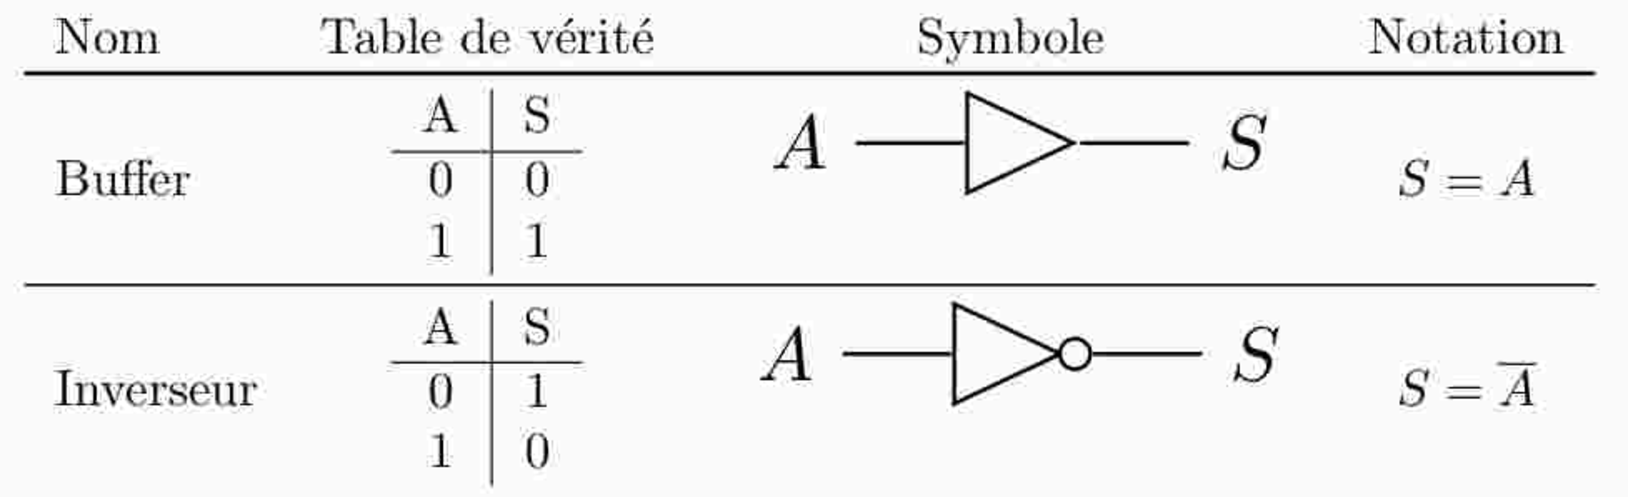
\includegraphics[width=0.5\linewidth]{Figs/porte1ent.pdf}
\end{block}
\begin{block}{Portes à 2 entrées}
\centering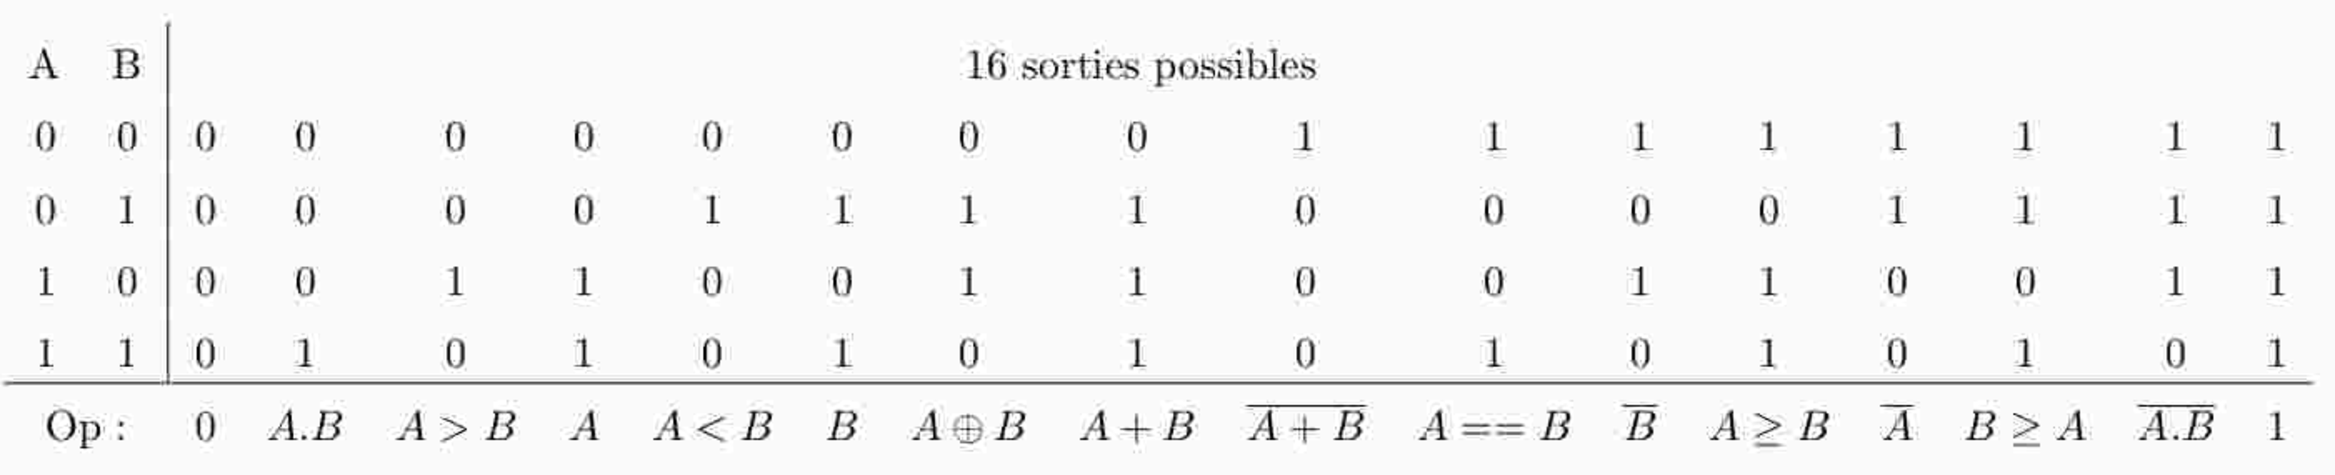
\includegraphics[width=\linewidth]{Figs/porte2ent.pdf}
\end{block}
\end{frame}

%%%%%%%%%%%%%%%%%%%%%%%%%%%%
\subsection{Synthèse}
\begin{frame}
\frametitle{Synthèse de circuits logiques}
\begin{block}{Les outils}
\begin{itemize}
\item Spécification fonctionnelle : table de vérité (e.g. $A + B$)
\item Equation logique et simplification (Tableau de Karnaugh) (e.g. $A + B$)
\item Disjonction de conjonctions
\item peut être réalisé 
  \begin{itemize}
  \item exclusivement avec des NAND,
  \item ou exclusivement avec des NOR
  \item exclusivement avec des NOT, AND, OR
  \end{itemize}
\end{itemize}
\end{block}
\end{frame}

\begin{frame}
  \frametitle{Circuits à $n > 2$ entrées}
  \begin{block}{Cascade/Arbre et temps de propagation}
    Exemple d'une porte ET à 4 entrées.\\
    \begin{minipage}[c]{.46\linewidth}
      \begin{overprint}
      \onslide<2->{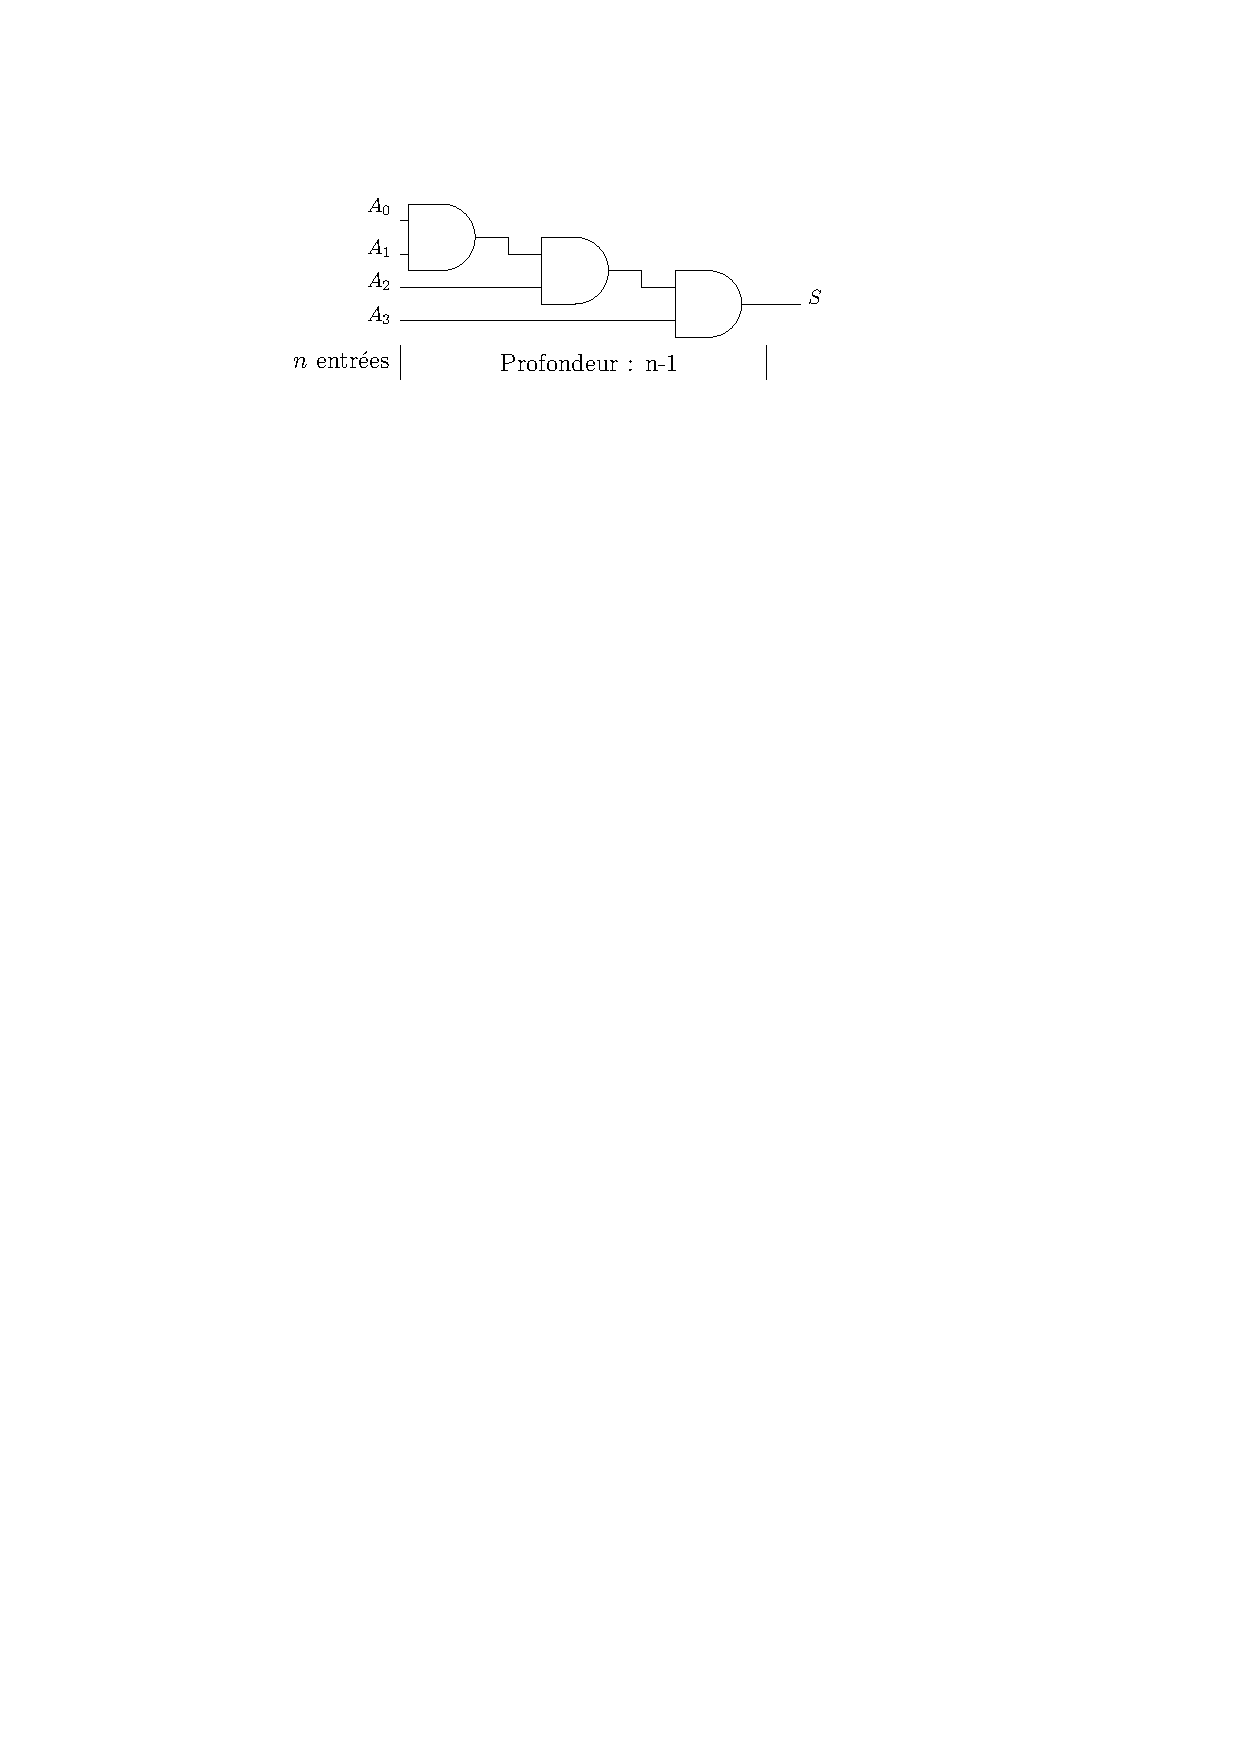
\includegraphics[width=\columnwidth]{Figs/and_4e_cascade.pdf}}
      \onslide<4->{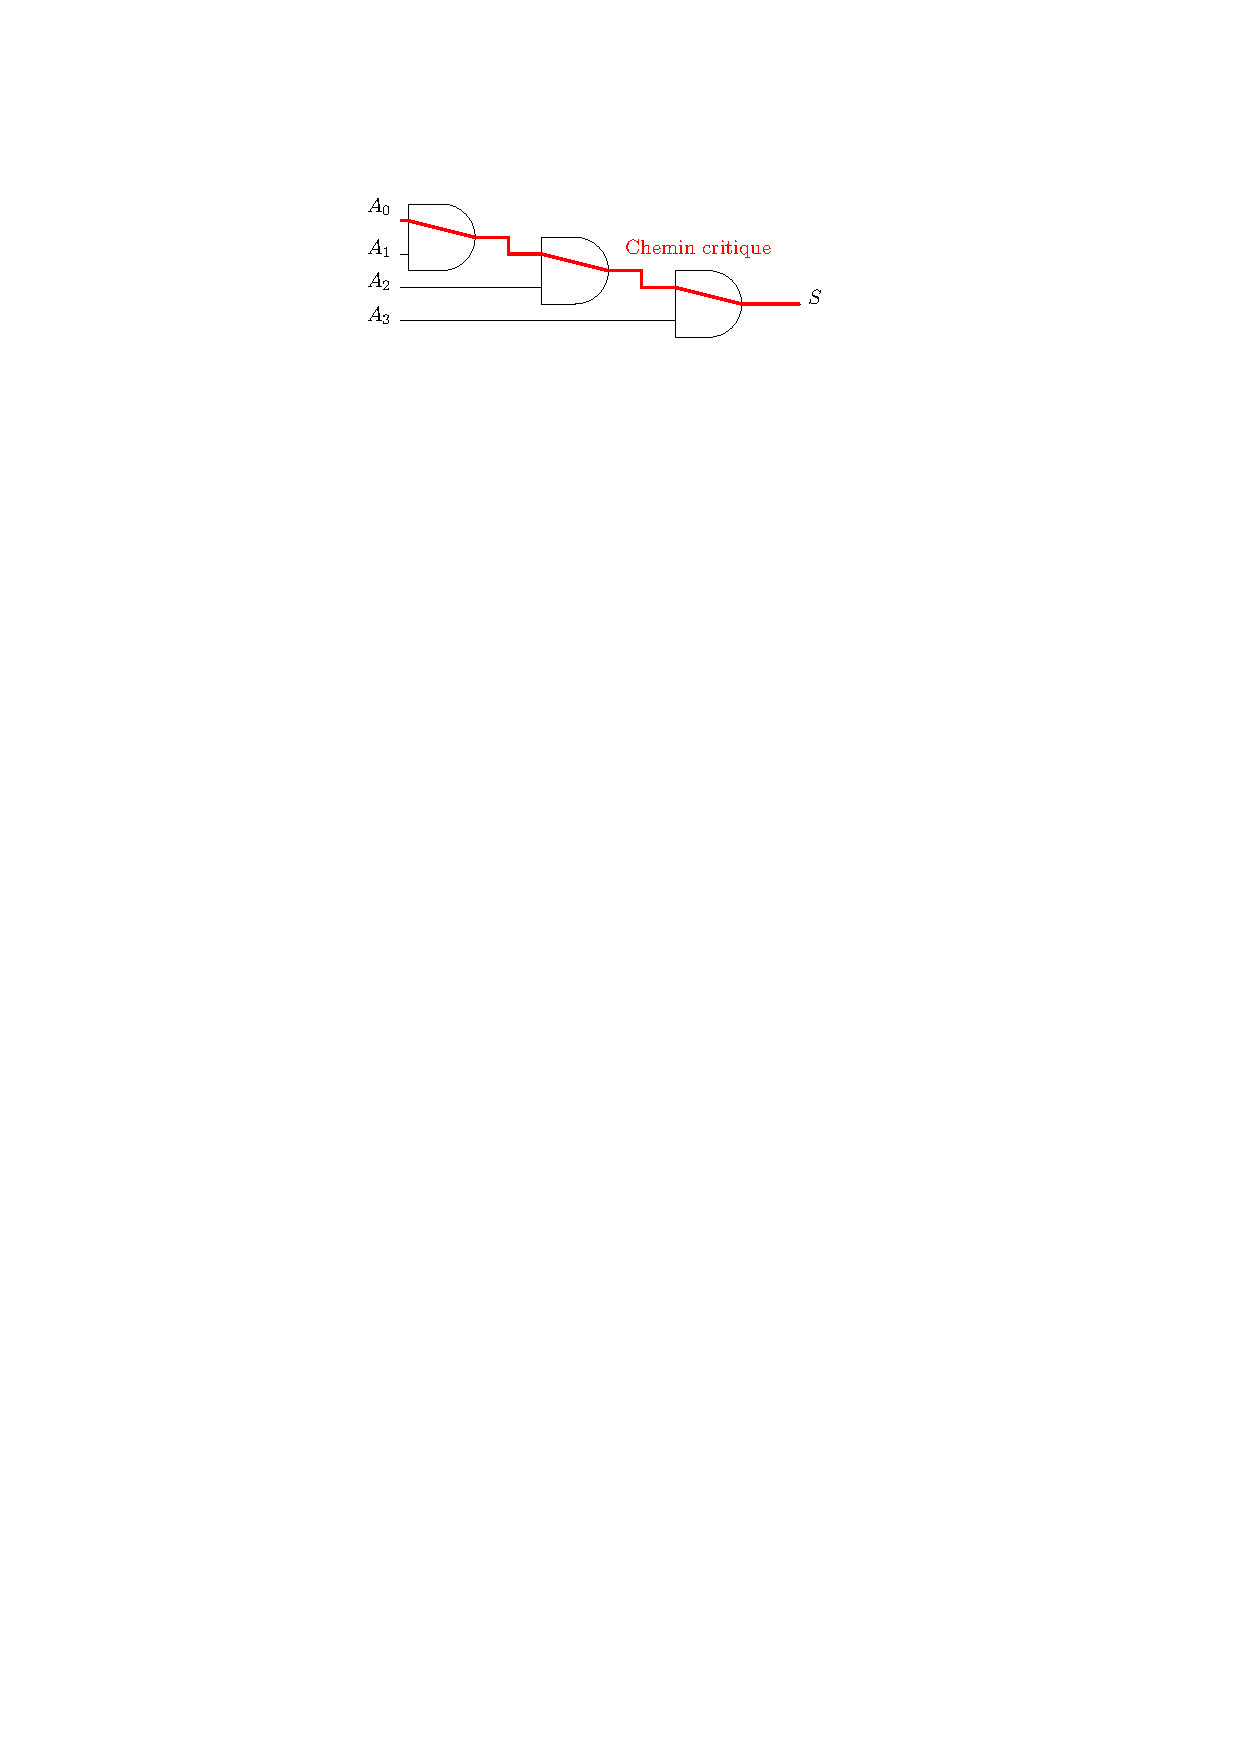
\includegraphics[width=\columnwidth]{Figs/and_4e_cascade_critique.pdf}}
      \end{overprint}
    \end{minipage}
    \begin{minipage}[c]{.46\linewidth}
      \begin{overprint}
      \onslide<3->{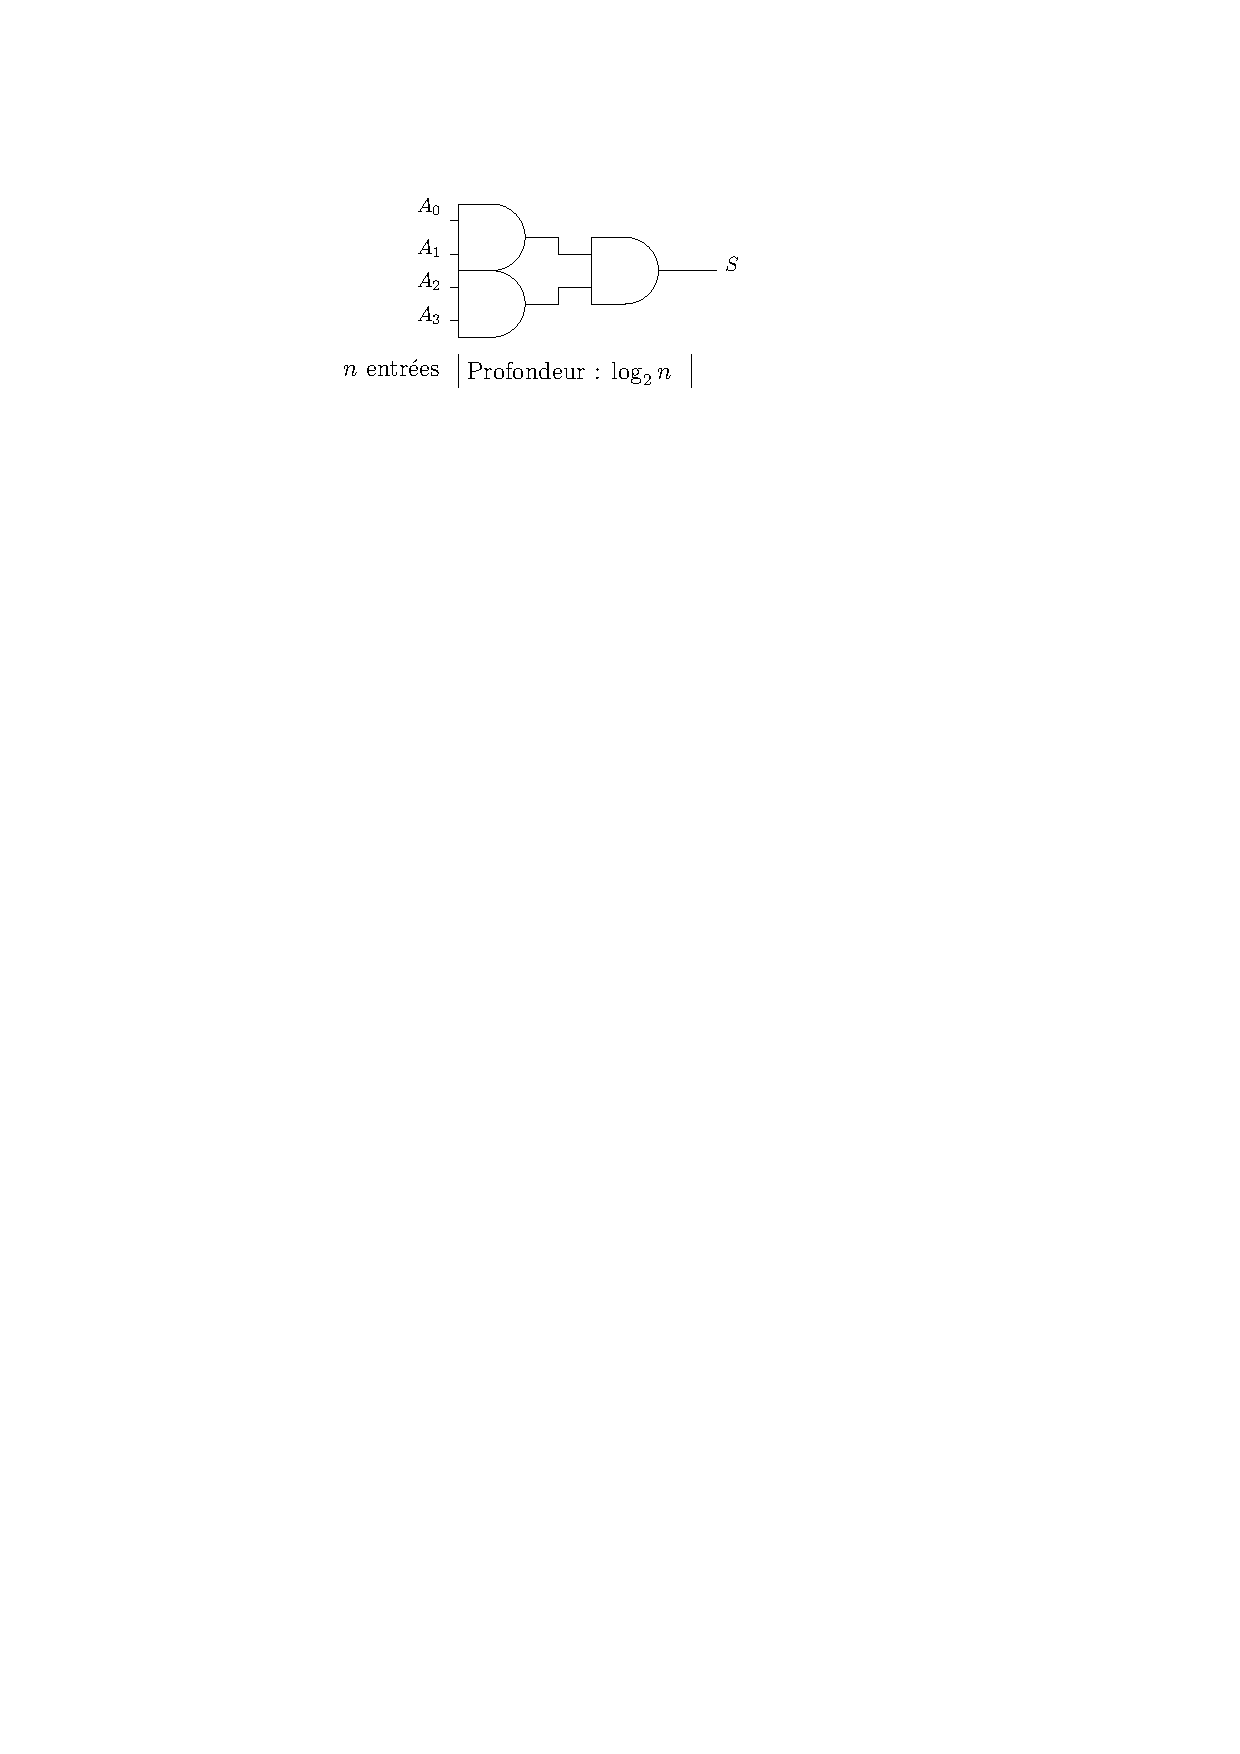
\includegraphics[width=\columnwidth]{Figs/and_4e_arbre.pdf}}
      \onslide<5->{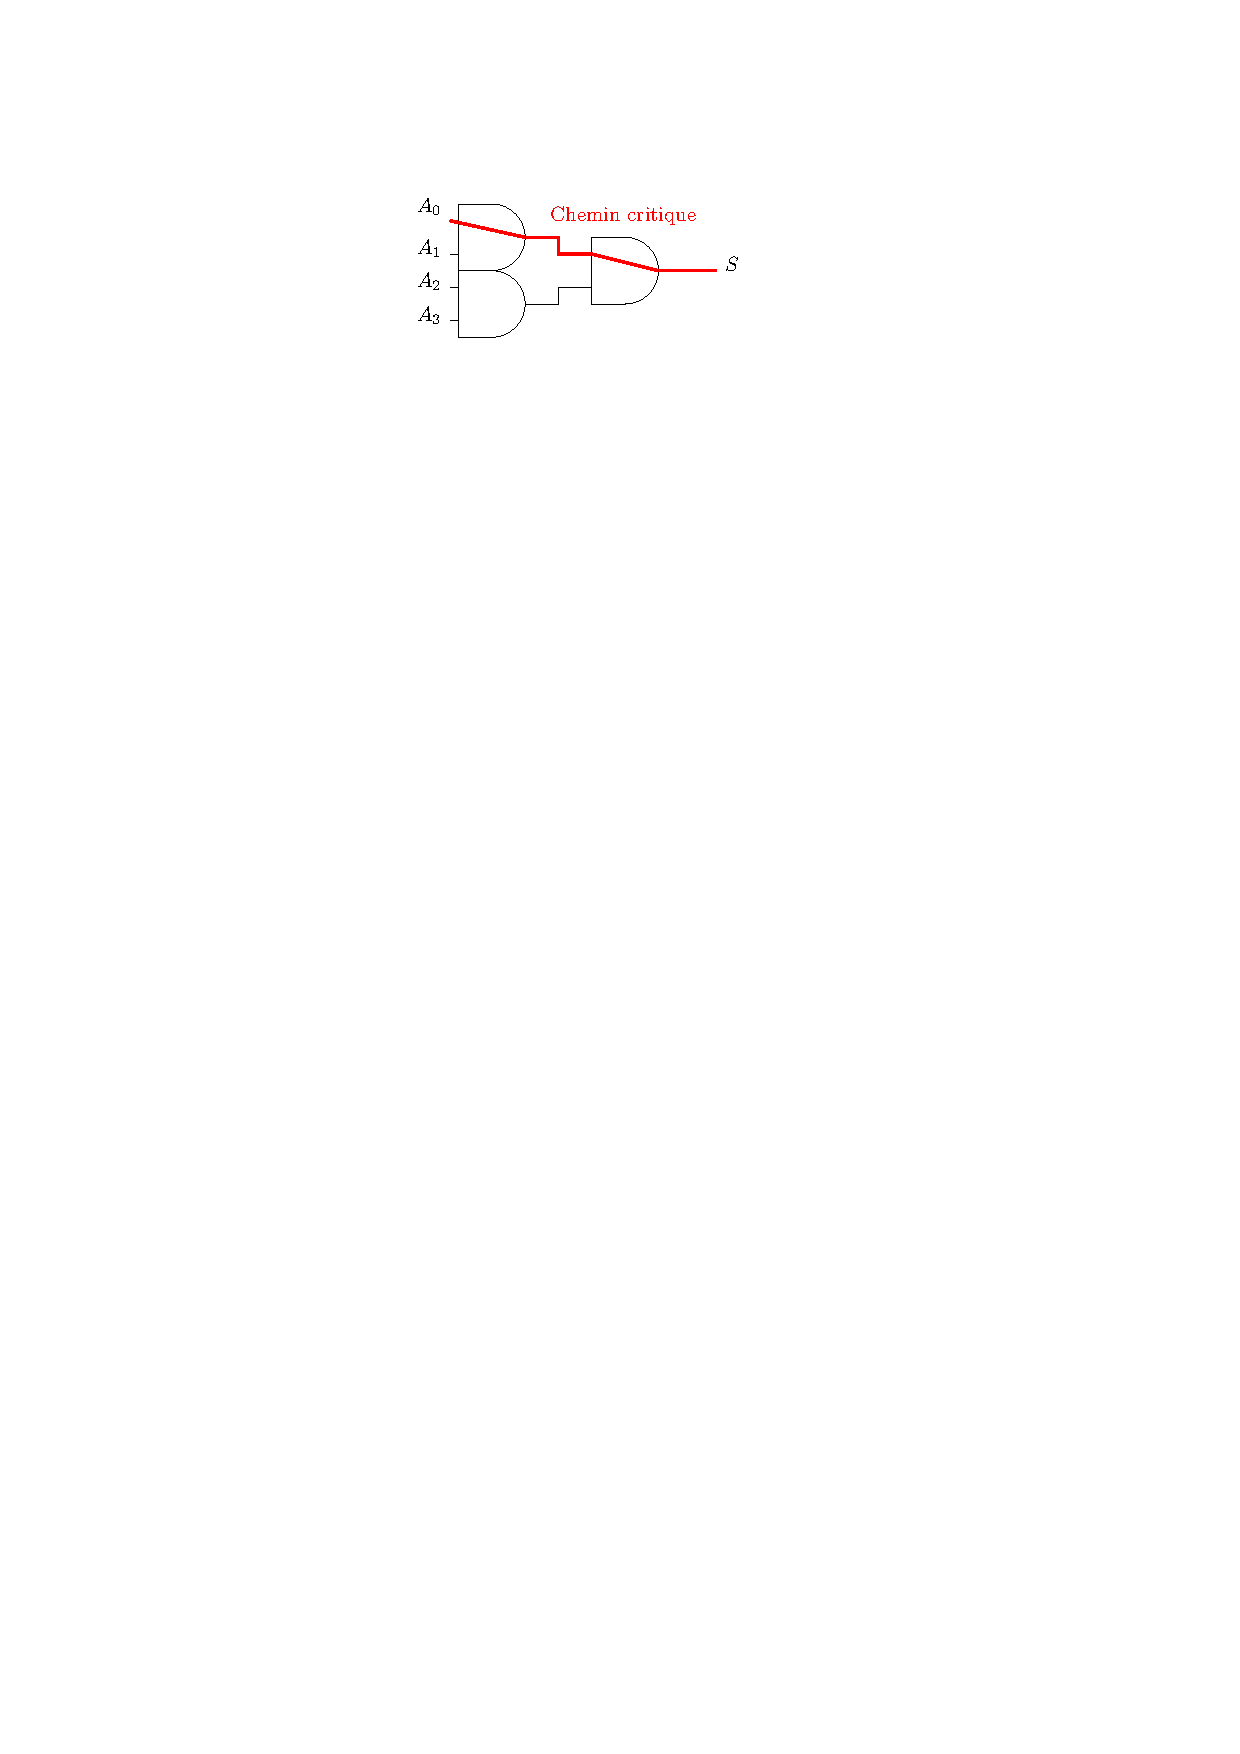
\includegraphics[width=\columnwidth]{Figs/and_4e_arbre_critique.pdf}}
      \end{overprint}
    \end{minipage}
  \end{block}
\end{frame}

%% \begin{frame}
%%   \frametitle{Circuits à $n > 2$ entrées}
%%   \begin{block}{Cascade/Arbre et temps de propagation}
%%     Exemple d'une porte ET à 4 entrées.\\
%%     \begin{overlayarea}{0.46\columnwidth}{0.6\textheight}
%%       \includegraphics[width=\columnwidth]<2-3>{Figs/and_4e_cascade.pdf}
%%       \includegraphics[width=\columnwidth]<4->{Figs/and_4e_cascade_critique.pdf}
%%     \end{overlayarea}
%%     \begin{overlayarea}{0.46\columnwidth}{0.6\textheight}
%%       \includegraphics[width=\columnwidth]<3-4>{Figs/and_4e_arbre.pdf}
%%       \includegraphics[width=\columnwidth]<5->{Figs/and_4e_arbre_critique.pdf}
%%     \end{overlayarea}
%%   \end{block}
%% \end{frame}

%%%%%%%%%%%%%%%%%%%%%%%%%%%%
\subsection{Circuits combinatoires}

%% \begin{frame}
%% \frametitle{Circuits de logique combinatoire}

%% \begin{block}{Décodeur}
%% Spécification
%% \begin{itemize}
%% \item n entrées : $a_{n-1},\cdots,a_0$
%% \item $2^n$ sorties : $s_{2^n-1}, \cdots, s_0$
%% \item $s_i = 1$, $ i = (a_{n-1}\cdots a_0)_2$
%% \end{itemize}
%% \end{block}
%% \begin{block}{Spécification fonctionnelle $n=2$}
%% \begin{align*}
%% s_0 &= \bar{a_1}\bar{a_0}\\
%% s_1 &= \bar{a_1} a_0\\
%% s_2 &= a_1 \bara_0
%% \end{align*}
%% \end{block}

%% \end{frame}

\begin{frame}
\frametitle{Circuits de logique combinatoire}
\begin{block}{Décodeur}
$\Rightarrow$ Spécification fonctionnelle
\begin{center}
\begin{tabular}{cc}
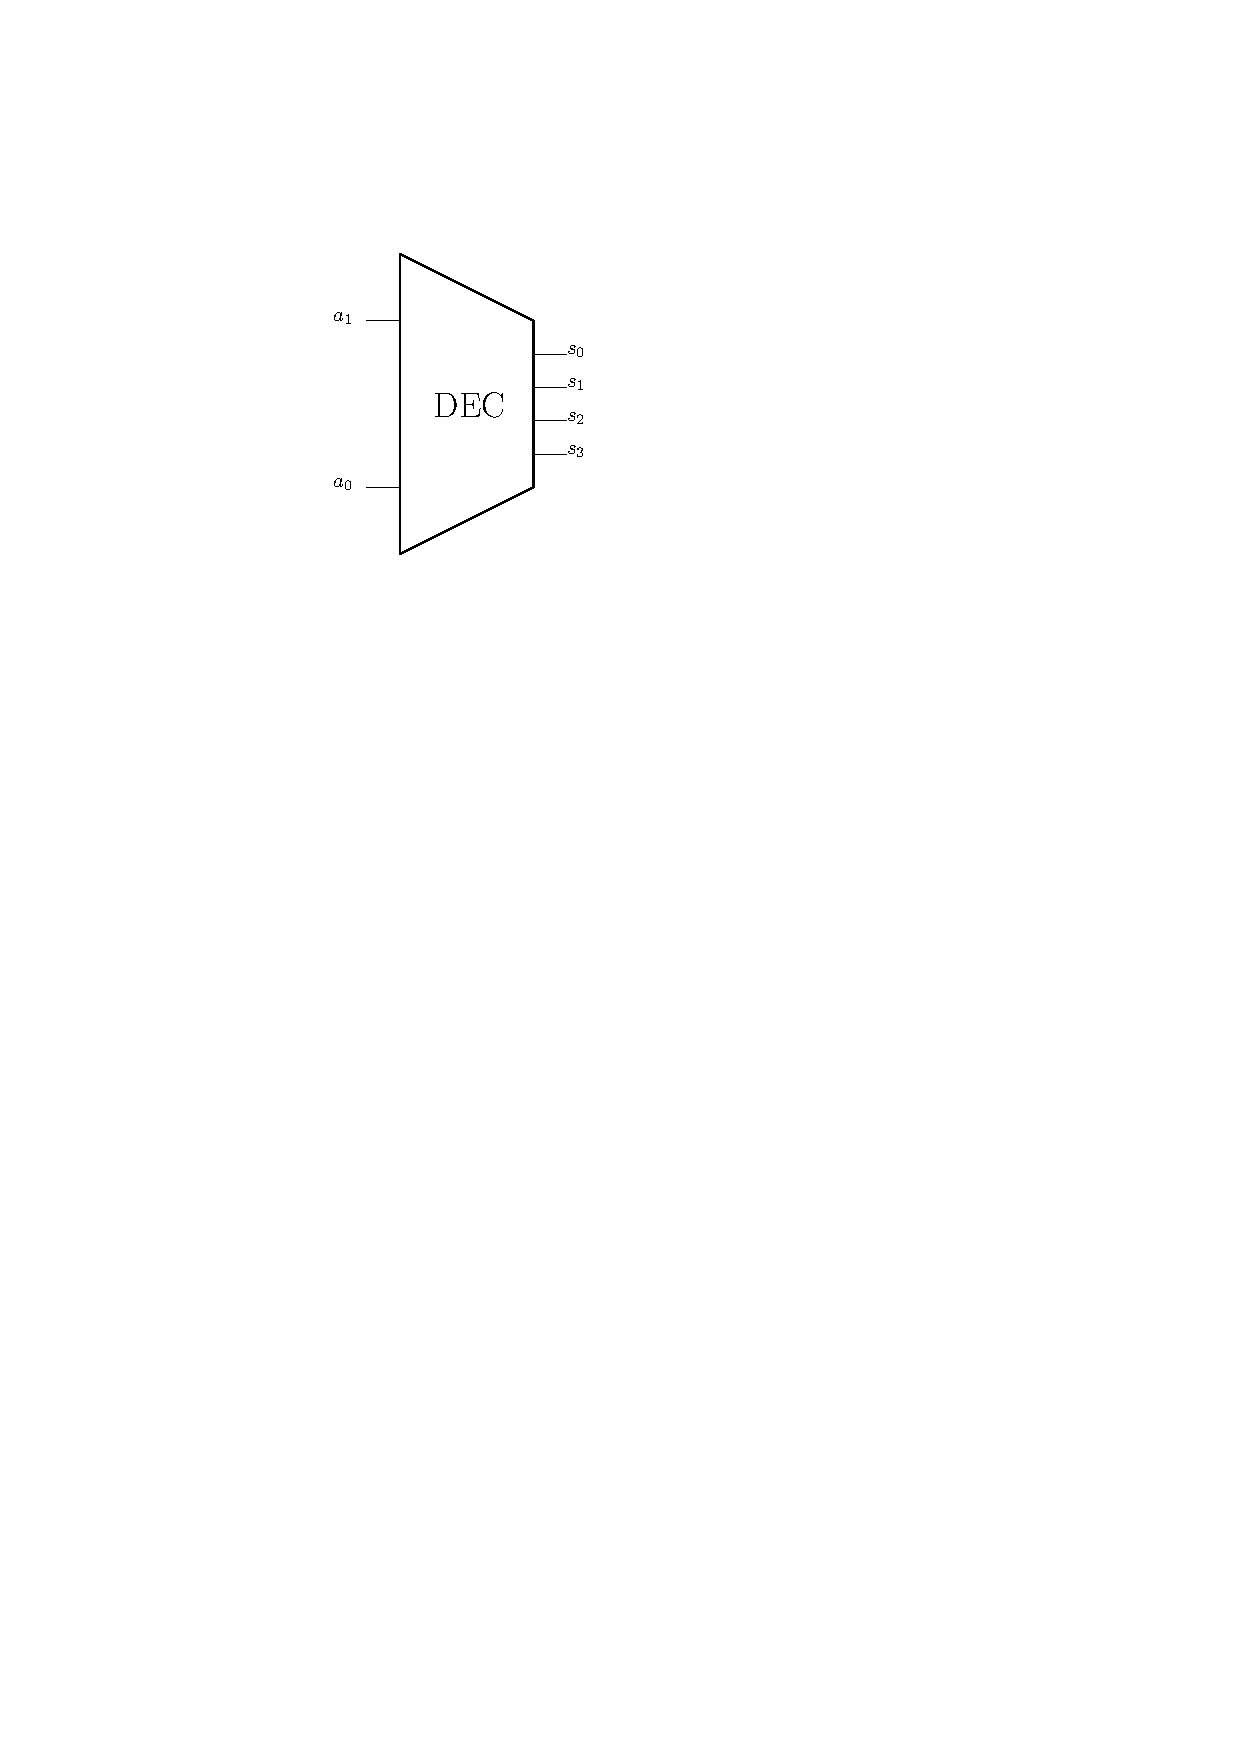
\includegraphics[width=0.25\linewidth]{Figs/dec.pdf} & 
\begin{circuitikz}[scale = 0.6, transform shape]
%\draw[very thin, gray](0,0) grid (11,11);
\draw[color=black,thick]
     (0,0) -- (0, 6) node[circ](A1){}
     (0, 6.5) node {$a_1$}
     (1, 5) node[not gate US,draw, logic gate inputs=n,rotate=-90] (NotA1) {}
     (0, 6) |- (1,5.5) -- (NotA1.input)
     (NotA1.output) -- (1,0)


     (2,0) -- (2, 6) node[circ](A0) {}
     (2, 6.5) node {$a_0$}
     (3, 5) node[not gate US,draw, logic gate inputs=n,rotate=-90] (NotA0) {}
     (2, 6) |- (3,5.5) -- (NotA0.input)
     (NotA0.output) -- (3,0)


     (5, 4) node[and gate US, draw, logic gate inputs=nn] (And0) {}
     (NotA0.output) |- (And0.input 1) node [midway, circ] {}
     (NotA1.output) |- (And0.input 2) node [midway, circ] {}
     (And0.output) -- ($(And0.output) + (0.5,0)$) node[circ](A0out) {} 
     ($(A0out) + (0.5,0)$) node{$s_0$}

     (5, 3) node[and gate US, draw, logic gate inputs=nn] (And1) {}
     (A0) |- (And1.input 1) node [midway, circ] {}
     (NotA1.output) |- (And1.input 2) node [midway, circ] {}
     (And1.output) -- ($(And1.output) + (0.5,0)$) node[circ](A1out) {} 
     ($(A1out) + (0.5,0)$) node{$s_1$}

     (5, 2) node[and gate US, draw, logic gate inputs=nn] (And2) {}
     (NotA0.output) |- (And2.input 1) node [midway, circ] {}
     (A1) |- (And2.input 2) node [midway, circ] {}
     (And2.output) -- ($(And2.output) + (0.5,0)$) node[circ](A2out) {} 
     ($(A2out) + (0.5,0)$) node{$s_2$}

     (5, 1) node[and gate US, draw, logic gate inputs=nn] (And3) {}
     (A0) |- (And3.input 1) node [midway, circ] {}
     (A1) |- (And3.input 2) node [midway, circ] {}
     (And3.output) -- ($(And3.output) + (0.5,0)$) node[circ](A3out) {} 
     ($(A3out) + (0.5,0)$) node{$s_3$}
;
\end{circuitikz} \\
a) & b)
\end{tabular}
\end{center}
\end{block}
\end{frame}

\begin{frame}
\frametitle{Circuits de logique combinatoire}
\begin{block}{Multiplexeur}
$\Rightarrow$ Spécification fonctionnelle\\

   \begin{minipage}[c]{.46\linewidth}
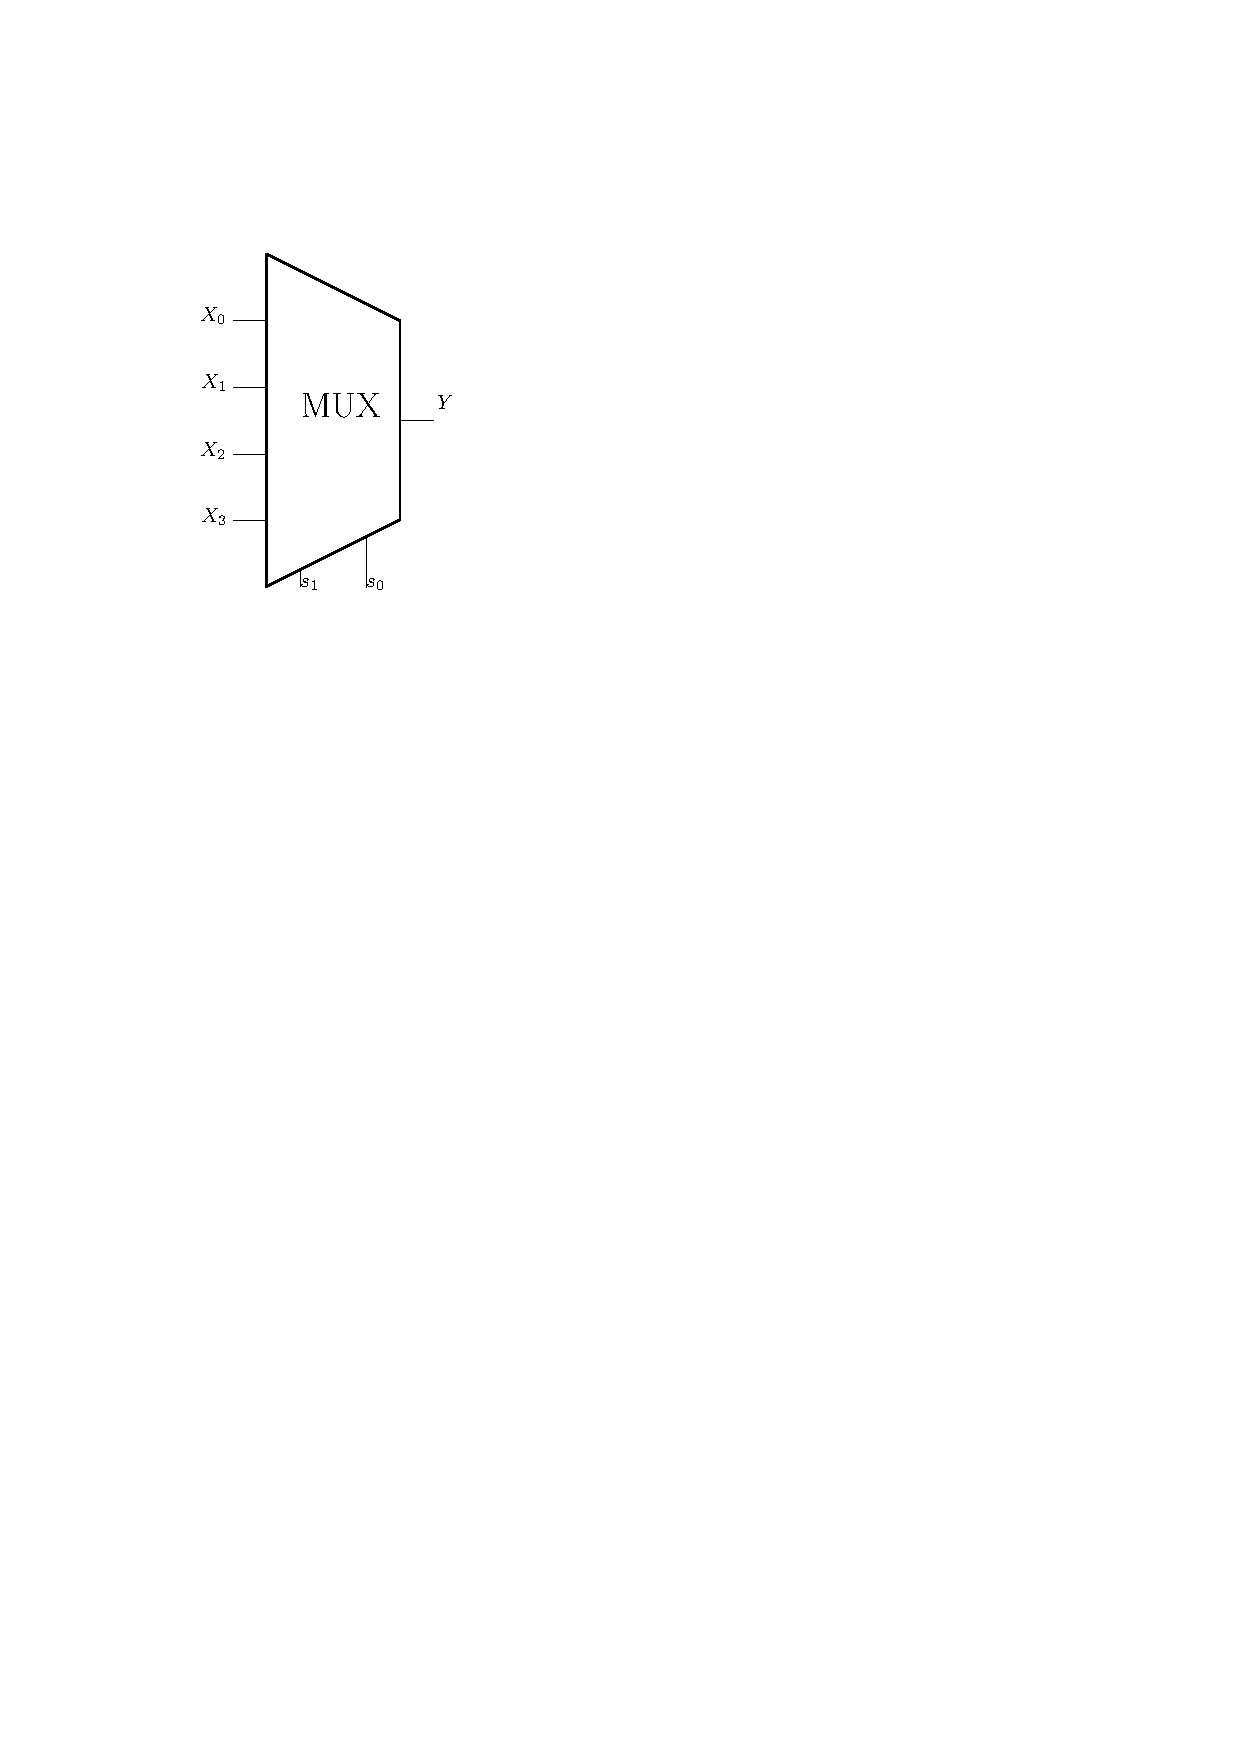
\includegraphics[width=0.5\linewidth]{Figs/mux.pdf} \\\centering a)
   \end{minipage} \hfill
   \begin{minipage}[c]{.46\linewidth}
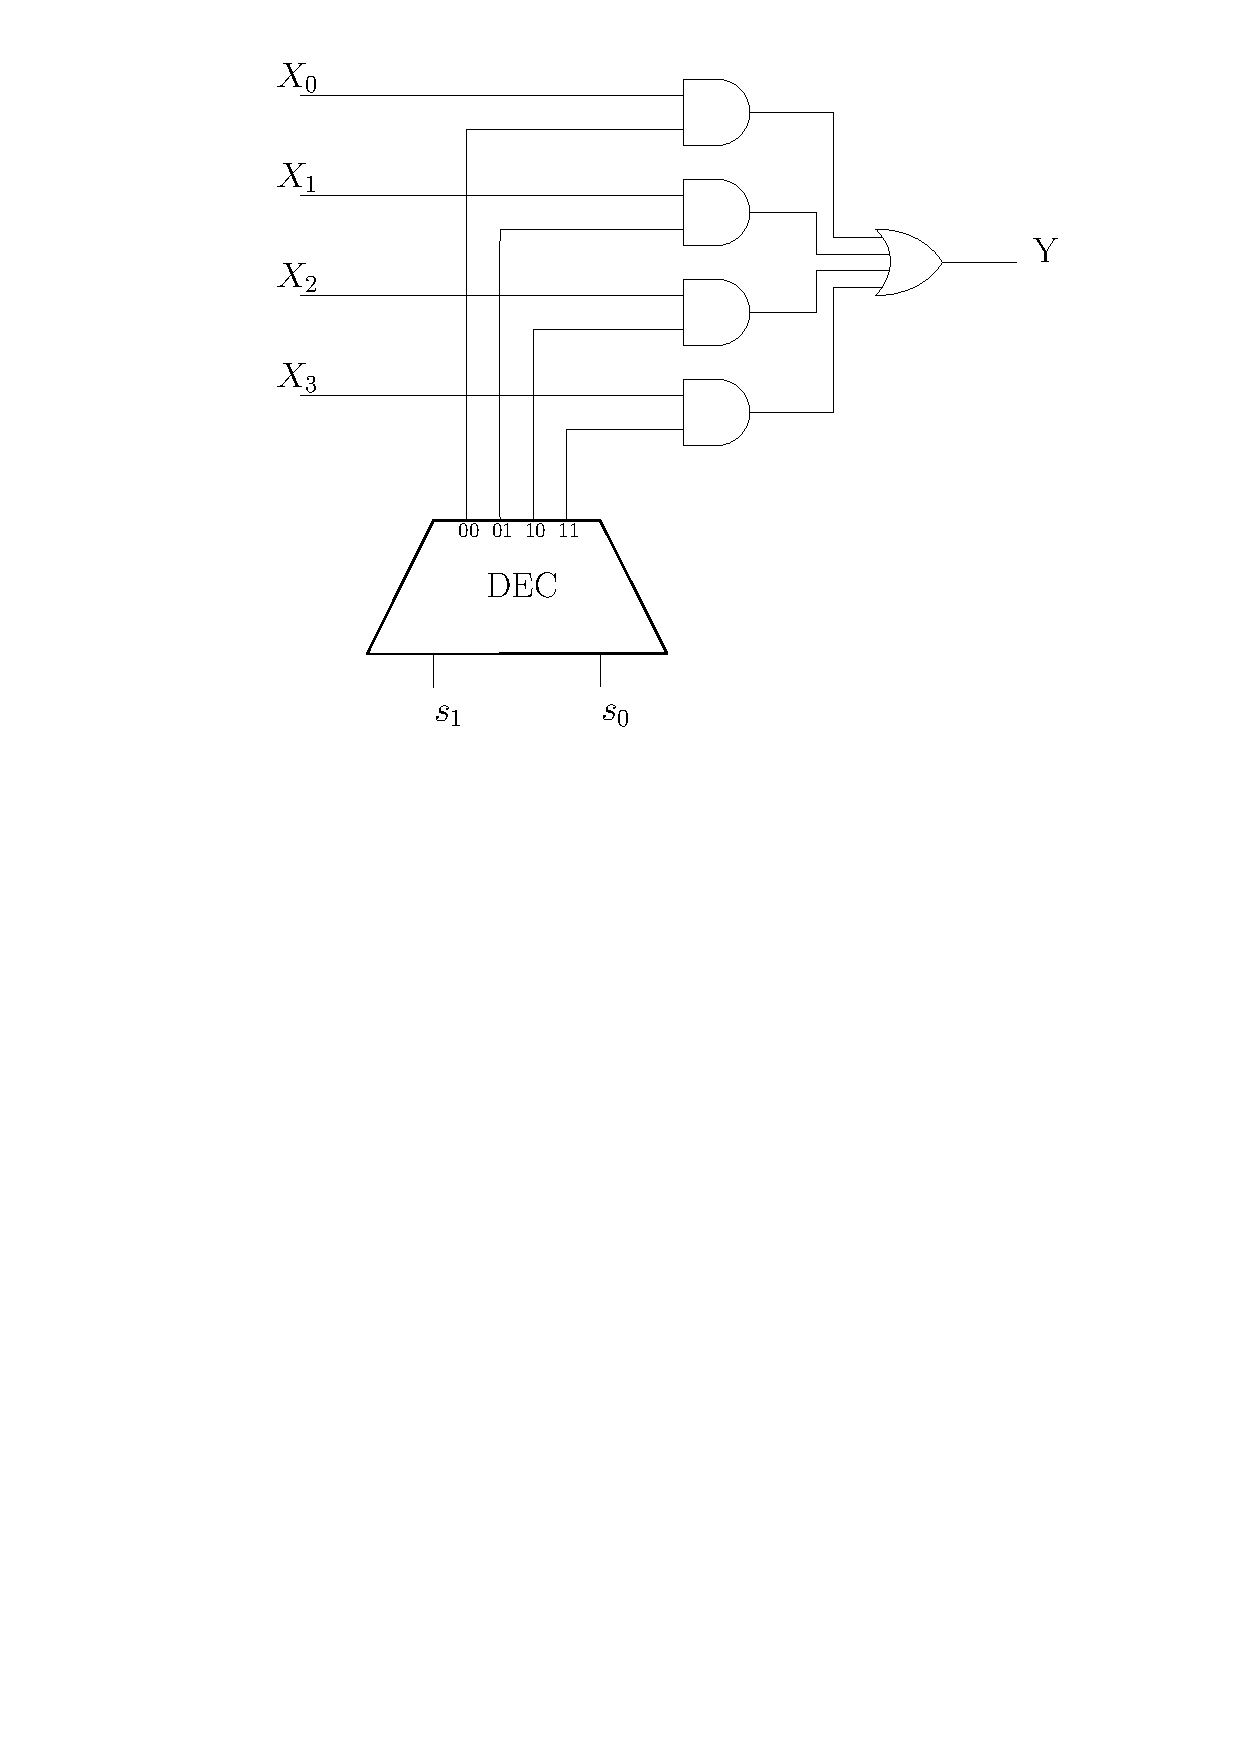
\includegraphics[width=\linewidth]{Figs/mux_inner.pdf}\\\centering b)
   \end{minipage}
\end{block}
\end{frame}

\begin{frame}
\frametitle{Circuits de logique combinatoire}
\begin{block}{Démultiplexeur}
$\Rightarrow$ Spécification fonctionnelle\\

   \begin{minipage}[c]{.46\linewidth}
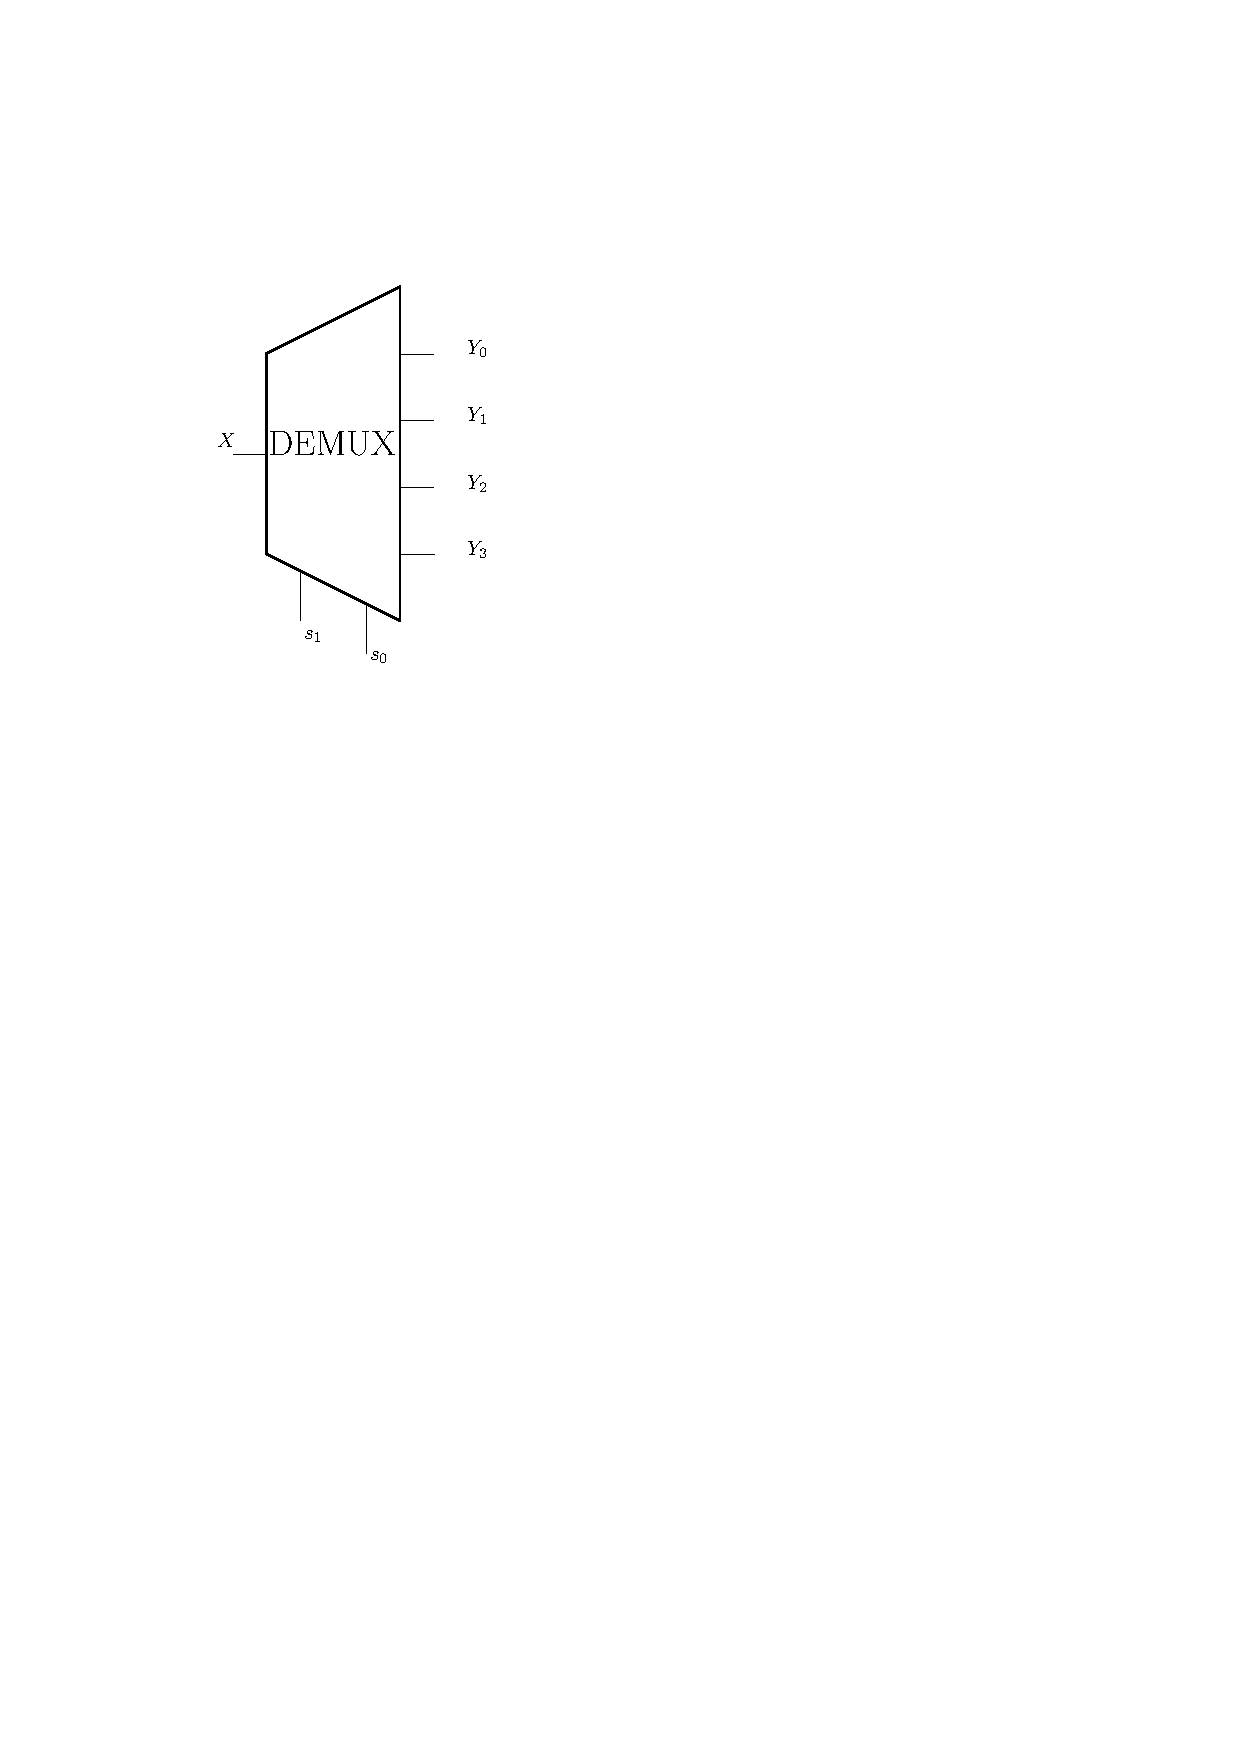
\includegraphics[width=0.5\linewidth]{Figs/demux.pdf} \\\centering a)
   \end{minipage} \hfill
   \begin{minipage}[c]{.46\linewidth}
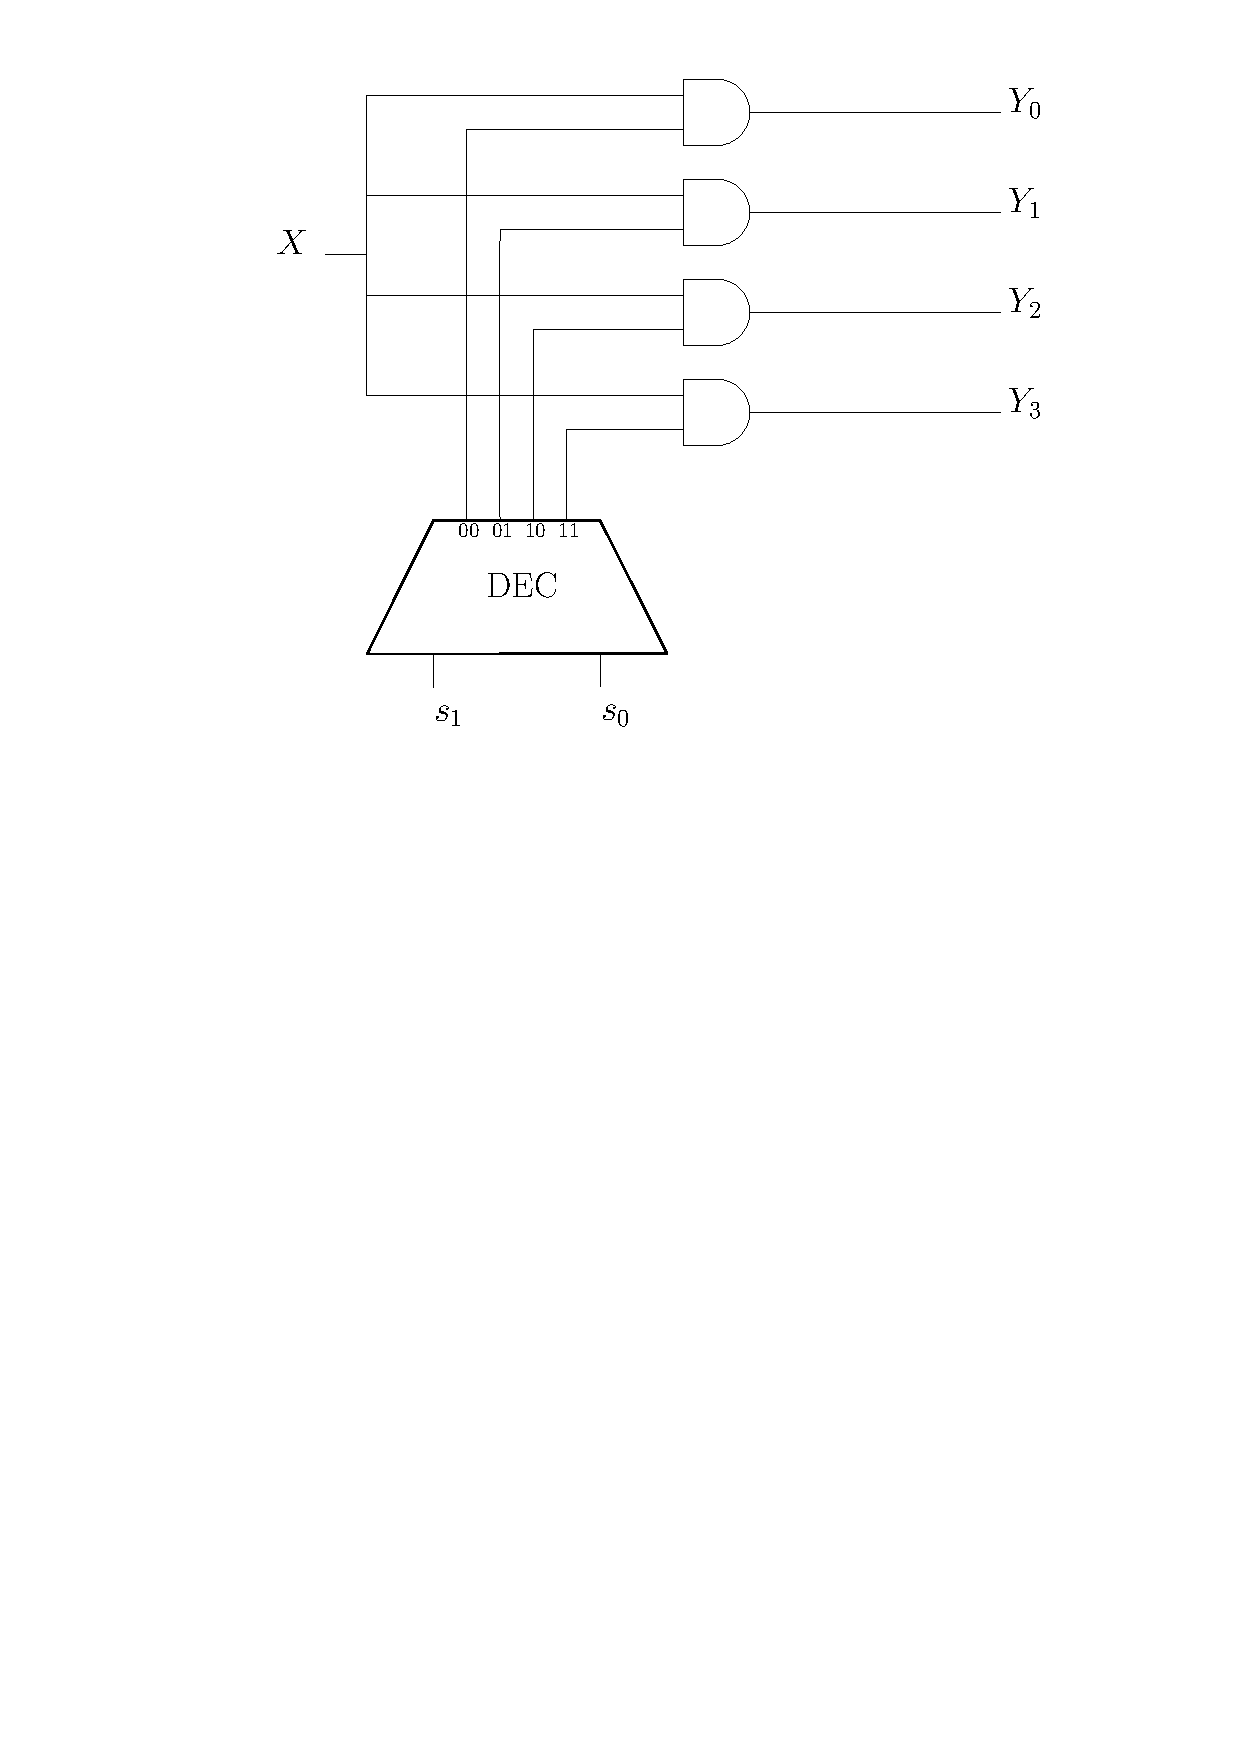
\includegraphics[width=\linewidth]{Figs/demux_inner.pdf}\\\centering b)
\end{minipage}
\end{block}
\end{frame}


\begin{frame}
\frametitle{Aléa statique}

\centering\begin{tabular}{c}
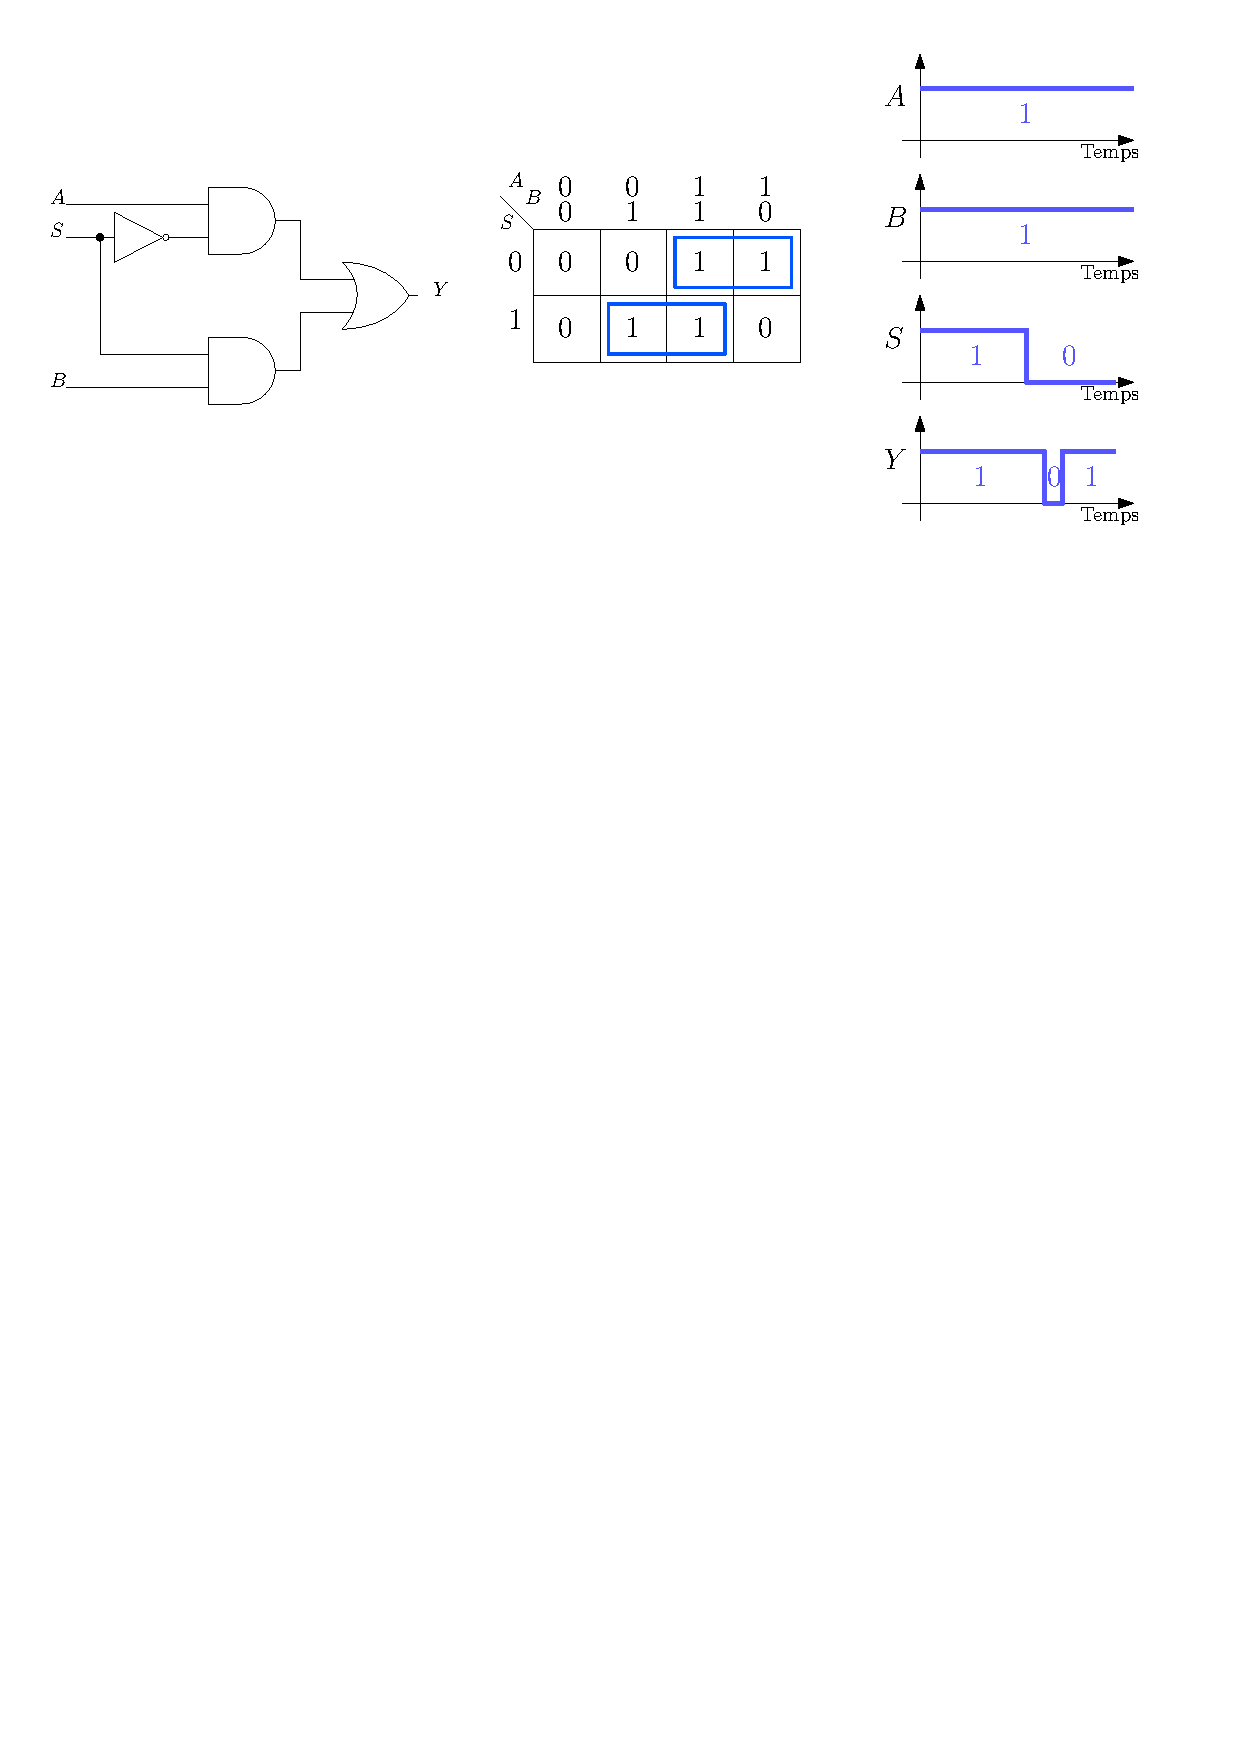
\includegraphics[width=0.7\linewidth]{Figs/and_2e_mux1.pdf}\\
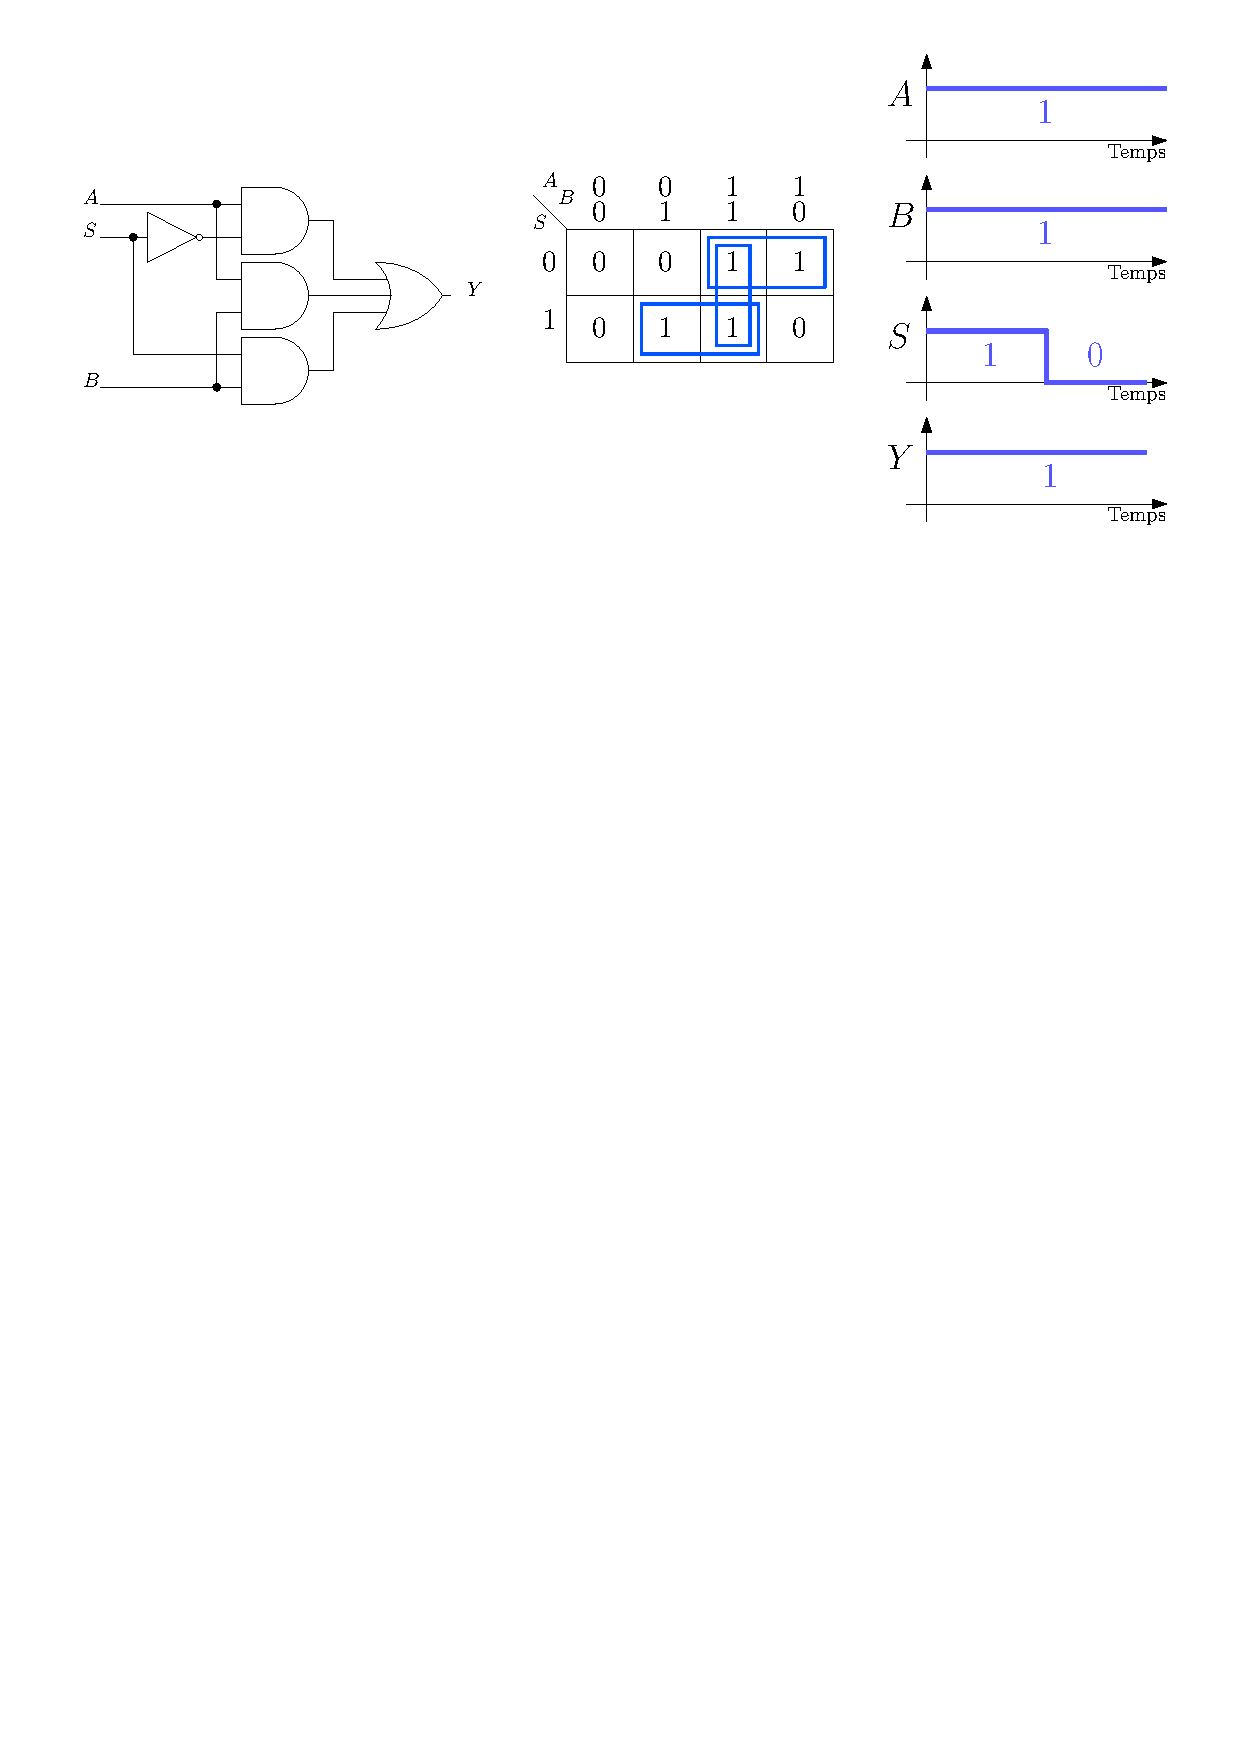
\includegraphics[width=0.7\linewidth]{Figs/and_2e_mux2.pdf}
\end{tabular}

\end{frame}

\begin{frame}
\frametitle{Universalité du multiplexeur et ROM}
\begin{block}{Universalité du multiplexeur}
   \begin{minipage}[c]{.4\linewidth}
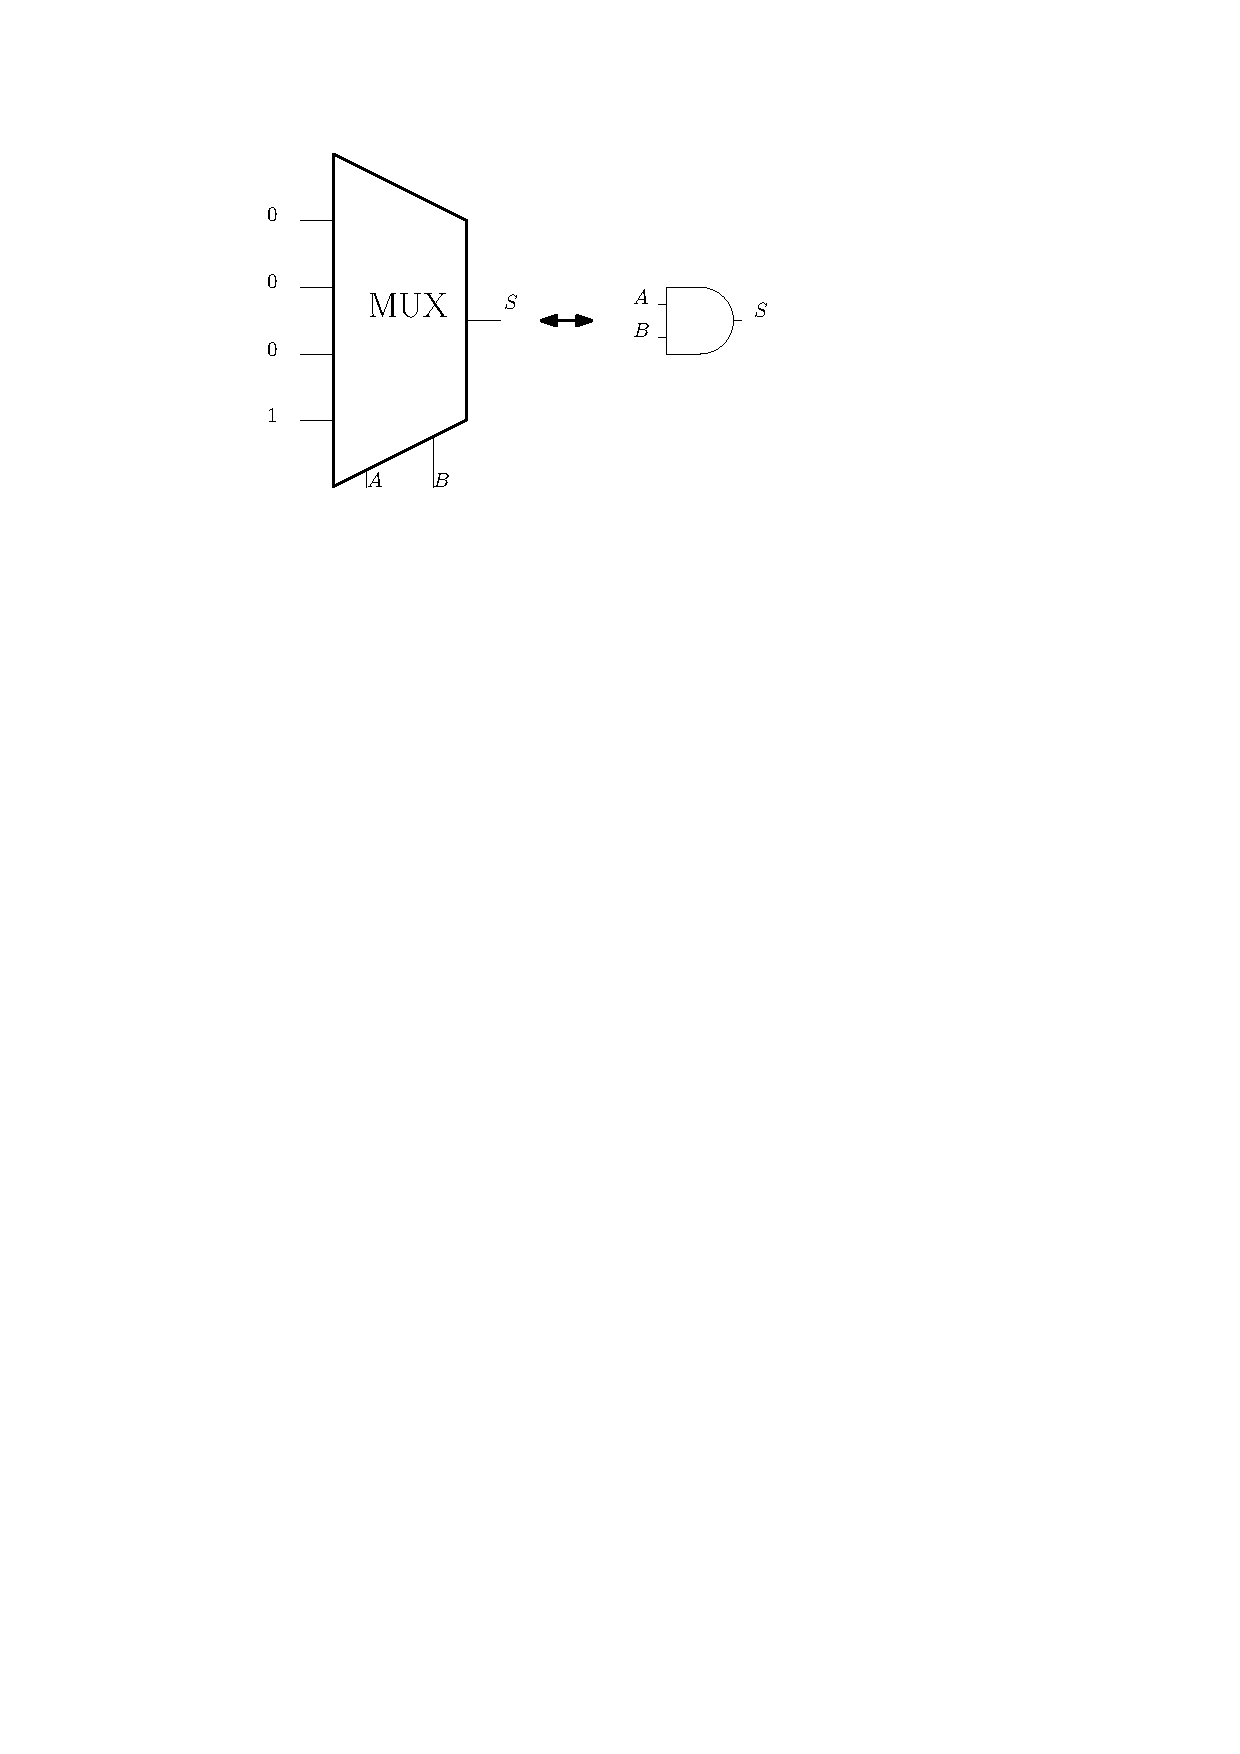
\includegraphics[width=\linewidth]{Figs/and_mux.pdf} \\\centering a)
   \end{minipage} \hfill
   \begin{minipage}[c]{0.4\linewidth}
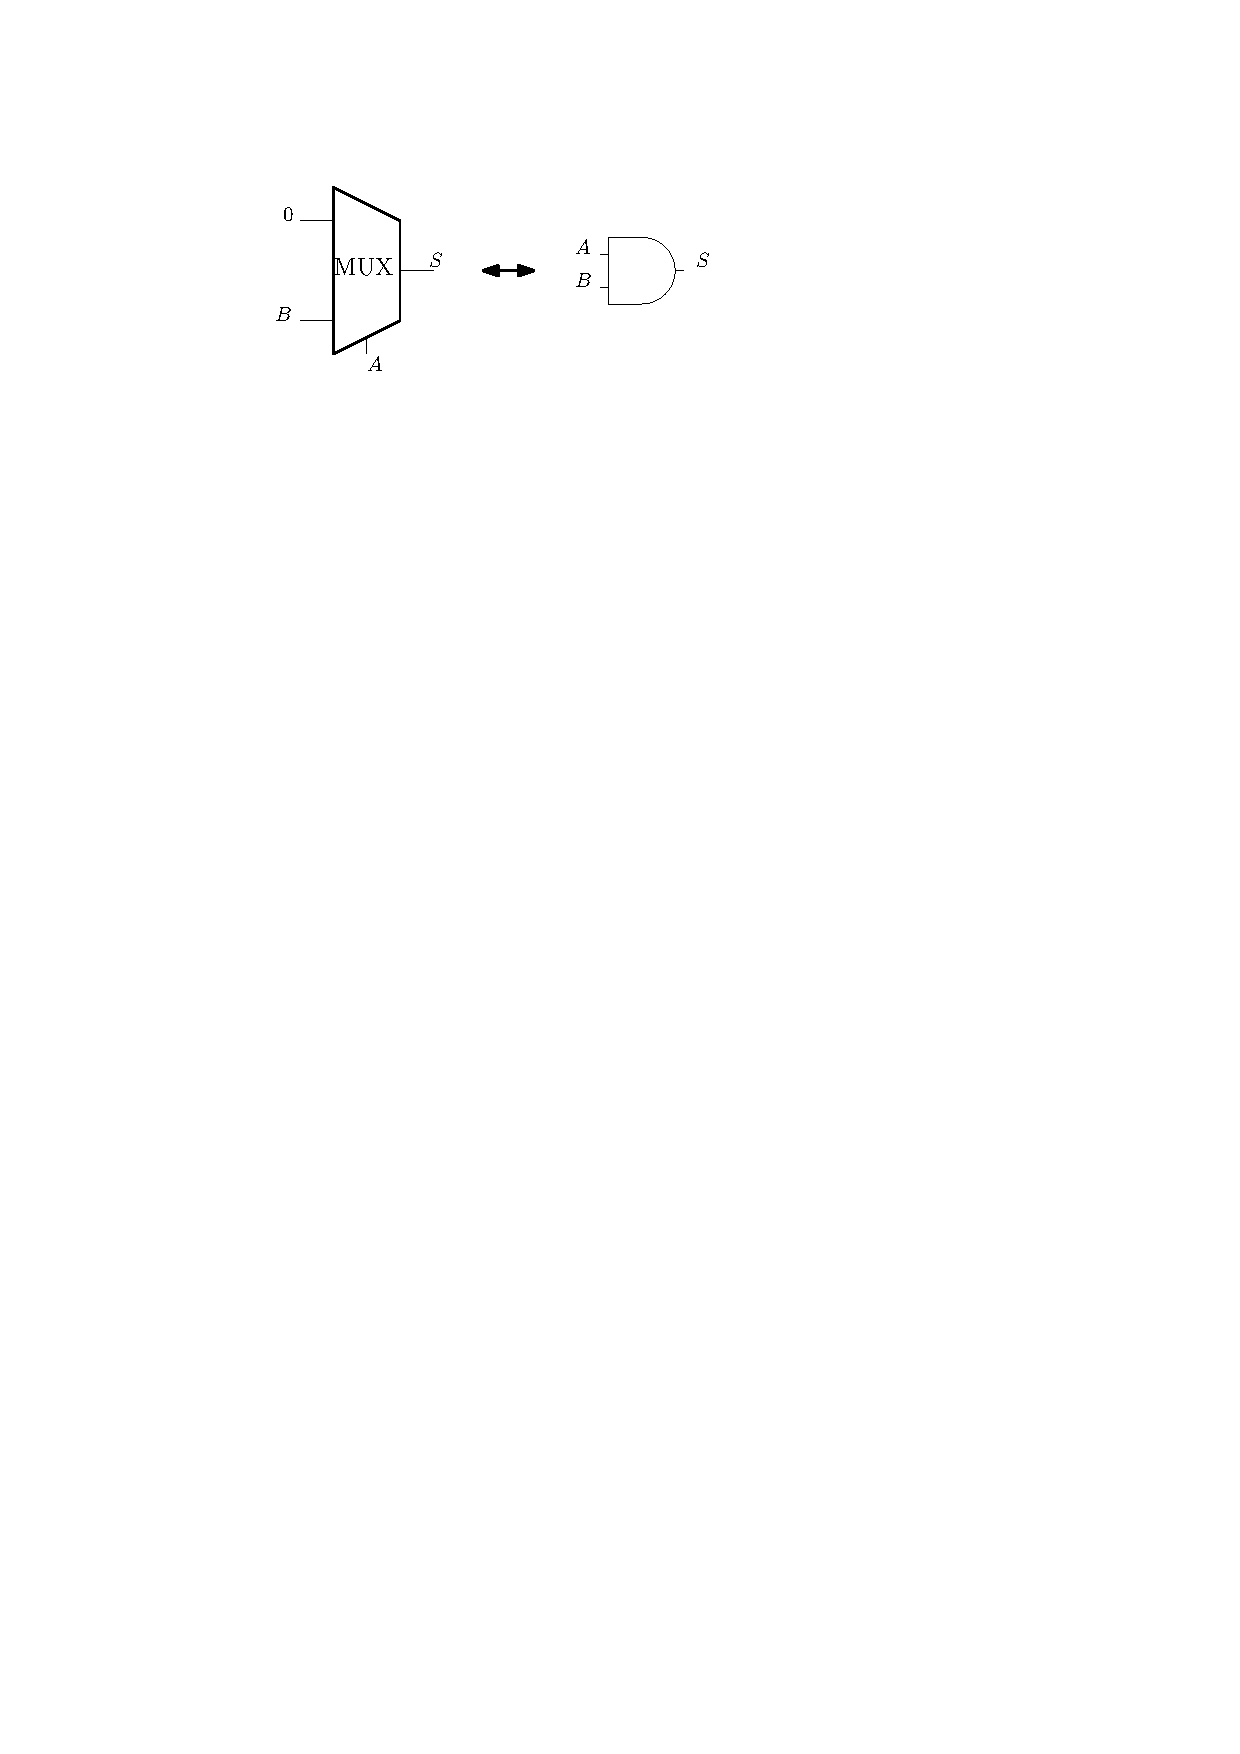
\includegraphics[width=\linewidth]{Figs/and_mux2.pdf}\\\centering b)
   \end{minipage}
\end{block}

$\Rightarrow$ Read Only Memory (ROM)
\end{frame}

\begin{frame}
\frametitle{Mémoire en lecture seule (Read Only Memory - ROM)}
\centering\includegraphics[width=\linewidth]{Figs/rom_inner.pdf}
\end{frame}

\begin{frame}
\frametitle{Unité arithmétique et logique (UAL)}
\begin{block}{Cahier des charges}
\begin{itemize}
\item composant logique avec :
\begin{itemize}
\item 2 entrées A, B sur $n$ bits
\item 1 sortie S sur $n$ bits
\item des bits de sélection d'opération, e.g. $2^4 = 16$ op: $U_3U_2U_1U_0$
\end{itemize}
\end{itemize}
\centering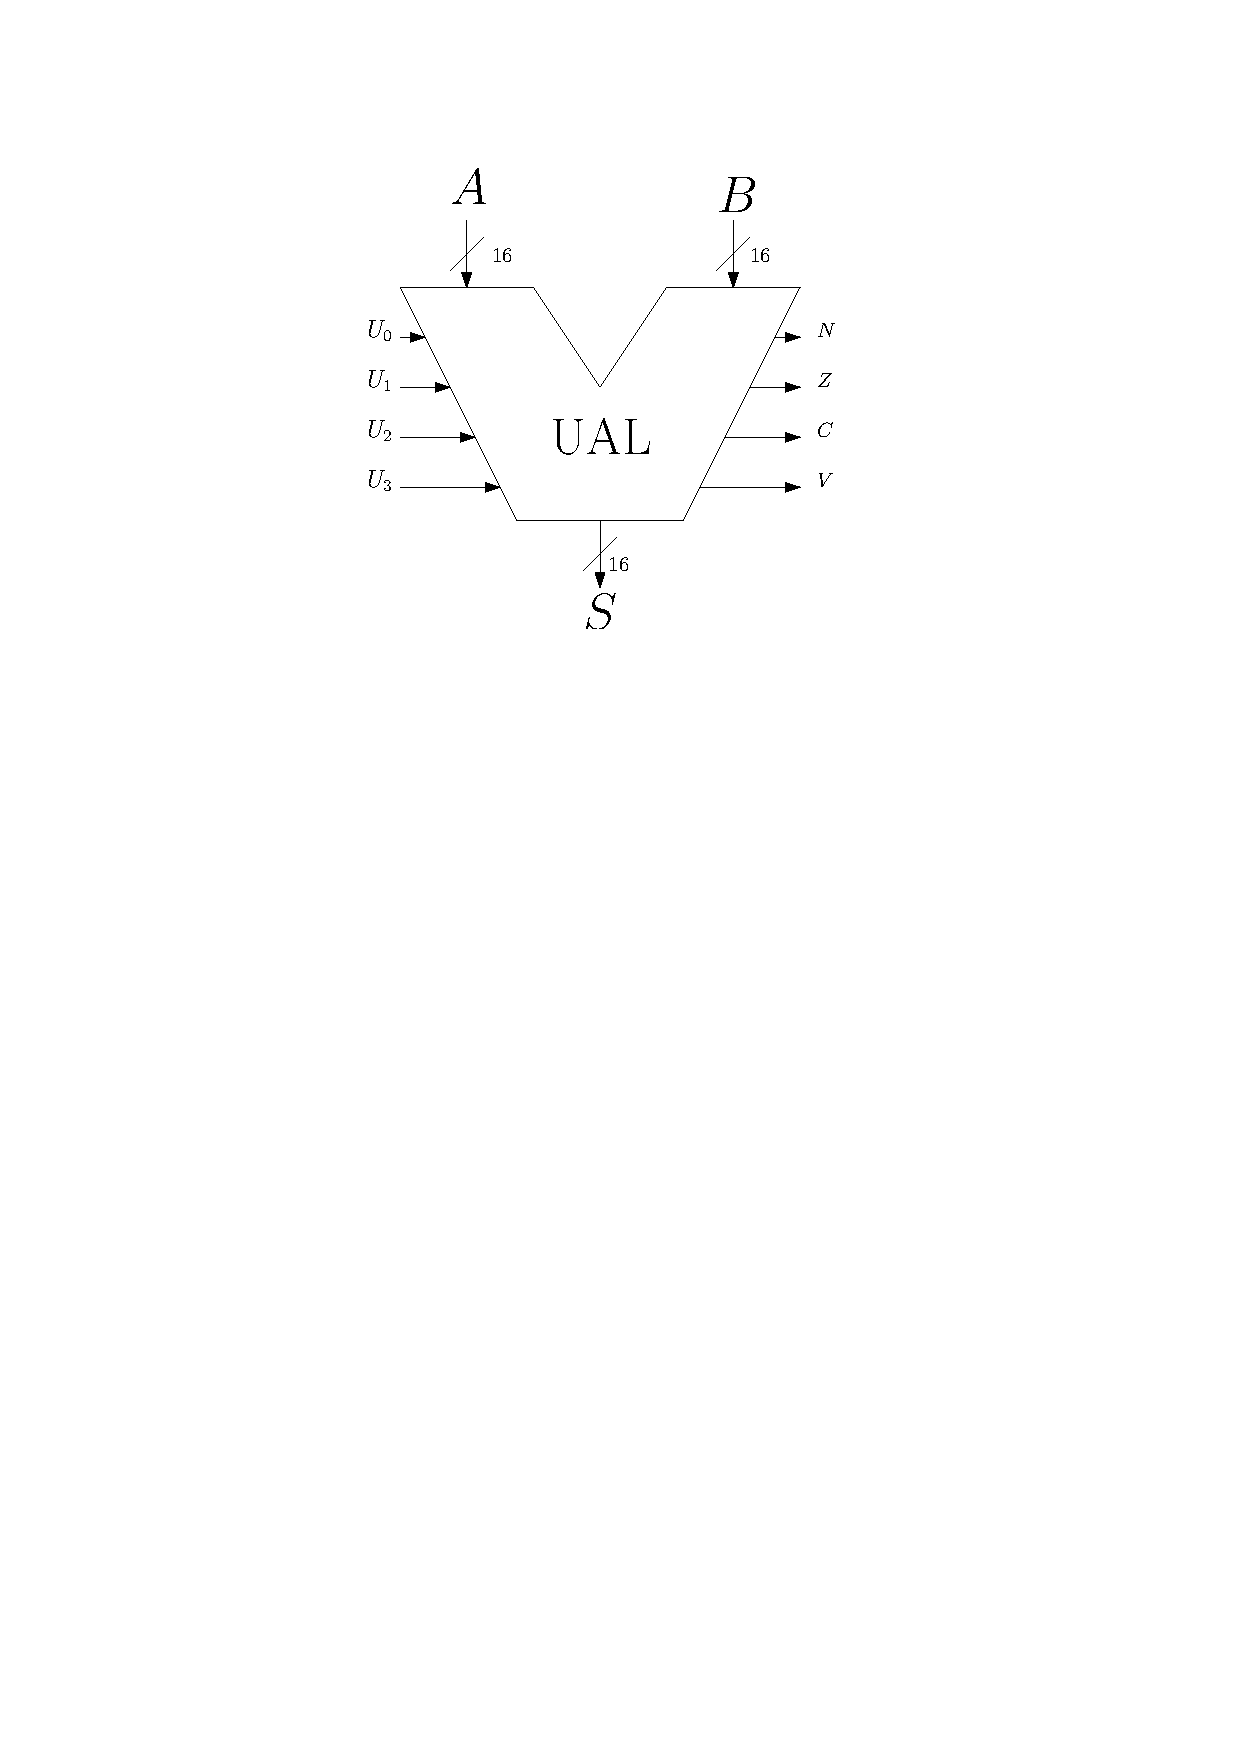
\includegraphics[width=0.3\linewidth]{Figs/ual.pdf}
\end{block}

\end{frame}

\begin{frame}
\frametitle{Unité arithmétique et logique (UAL) - Additionneur}
\begin{block}{Demi-additionneur 1 bit}
   \begin{minipage}[c]{.46\linewidth}
\begin{tabular}{cc|cc}
$a_i$ & $b_i$ & $s_i$ & $r$\\
\hline
0 & 0 & 0 & 0\\
0 & 1 & 1 & 0\\
1 & 0 & 1 & 0\\
1 & 1 & 0 & 1
\end{tabular}\\\centering a)
   \end{minipage} \hfill
   \begin{minipage}[c]{.46\linewidth}
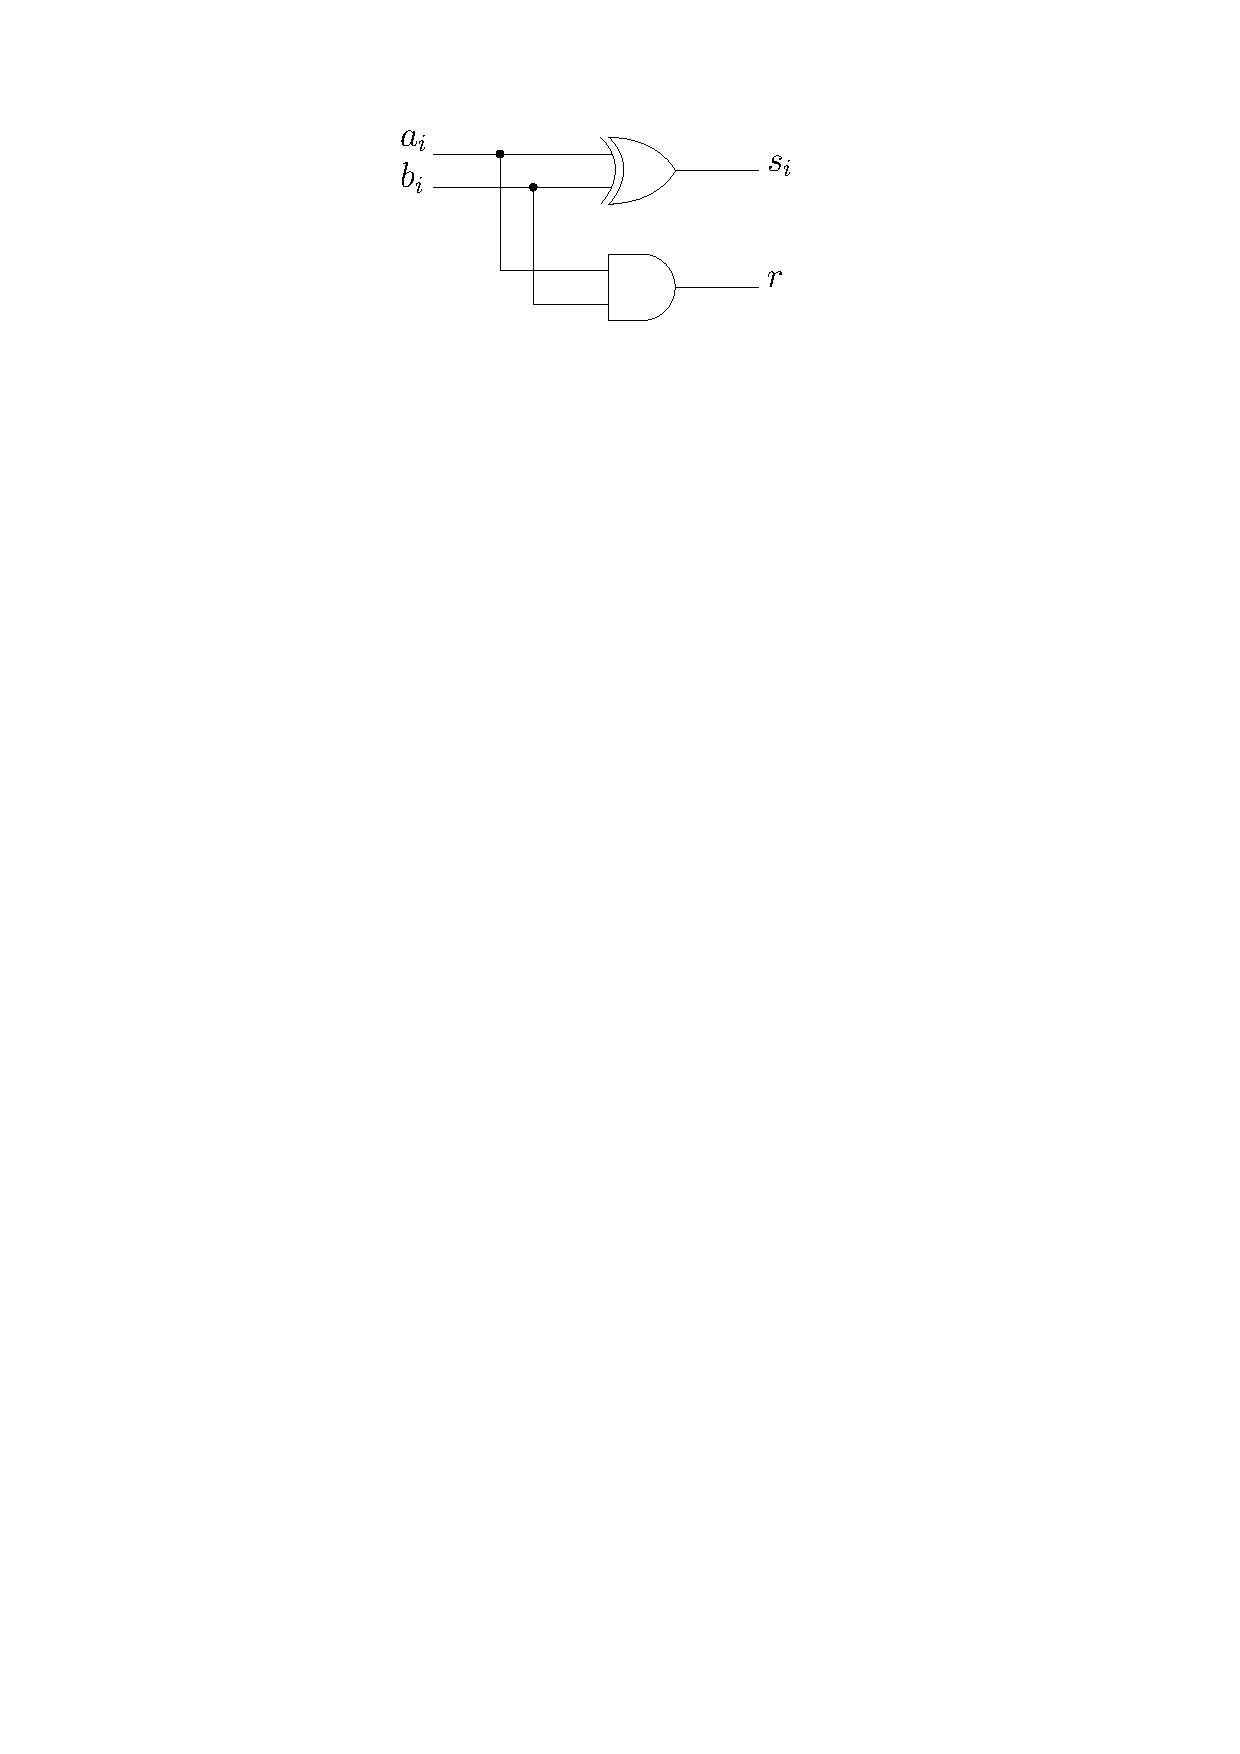
\includegraphics[width=\columnwidth]{Figs/half_adder.pdf}\\\centering b)
   \end{minipage}
\end{block}
\end{frame}


\begin{frame}
\frametitle{Unité arithmétique et logique (UAL) - Additionneur}
\begin{block}{Additionneur 1 bit}
  \begin{minipage}[c]{.46\linewidth}
\begin{tabular}{ccc|cc}
$a_i$ & $b_i$ & $r_i$ & $s_i$ & $r_{i+1}$\\
\hline
0 & 0 & 0& 0 & 0\\
0 & 0 & 1& 1 & 0\\
0 & 1 & 0 & 1 & 0\\
0 & 1 & 1 & 0 & 1\\
1 & 0 & 0 & 1 & 0\\
1 & 0 & 1 & 0 & 1\\
1 & 1 & 0 & 0 & 1\\
1 & 1 & 1 & 1 & 1
\end{tabular}\\\centering a)
   \end{minipage} \hfill
   \begin{minipage}[c]{.46\linewidth}
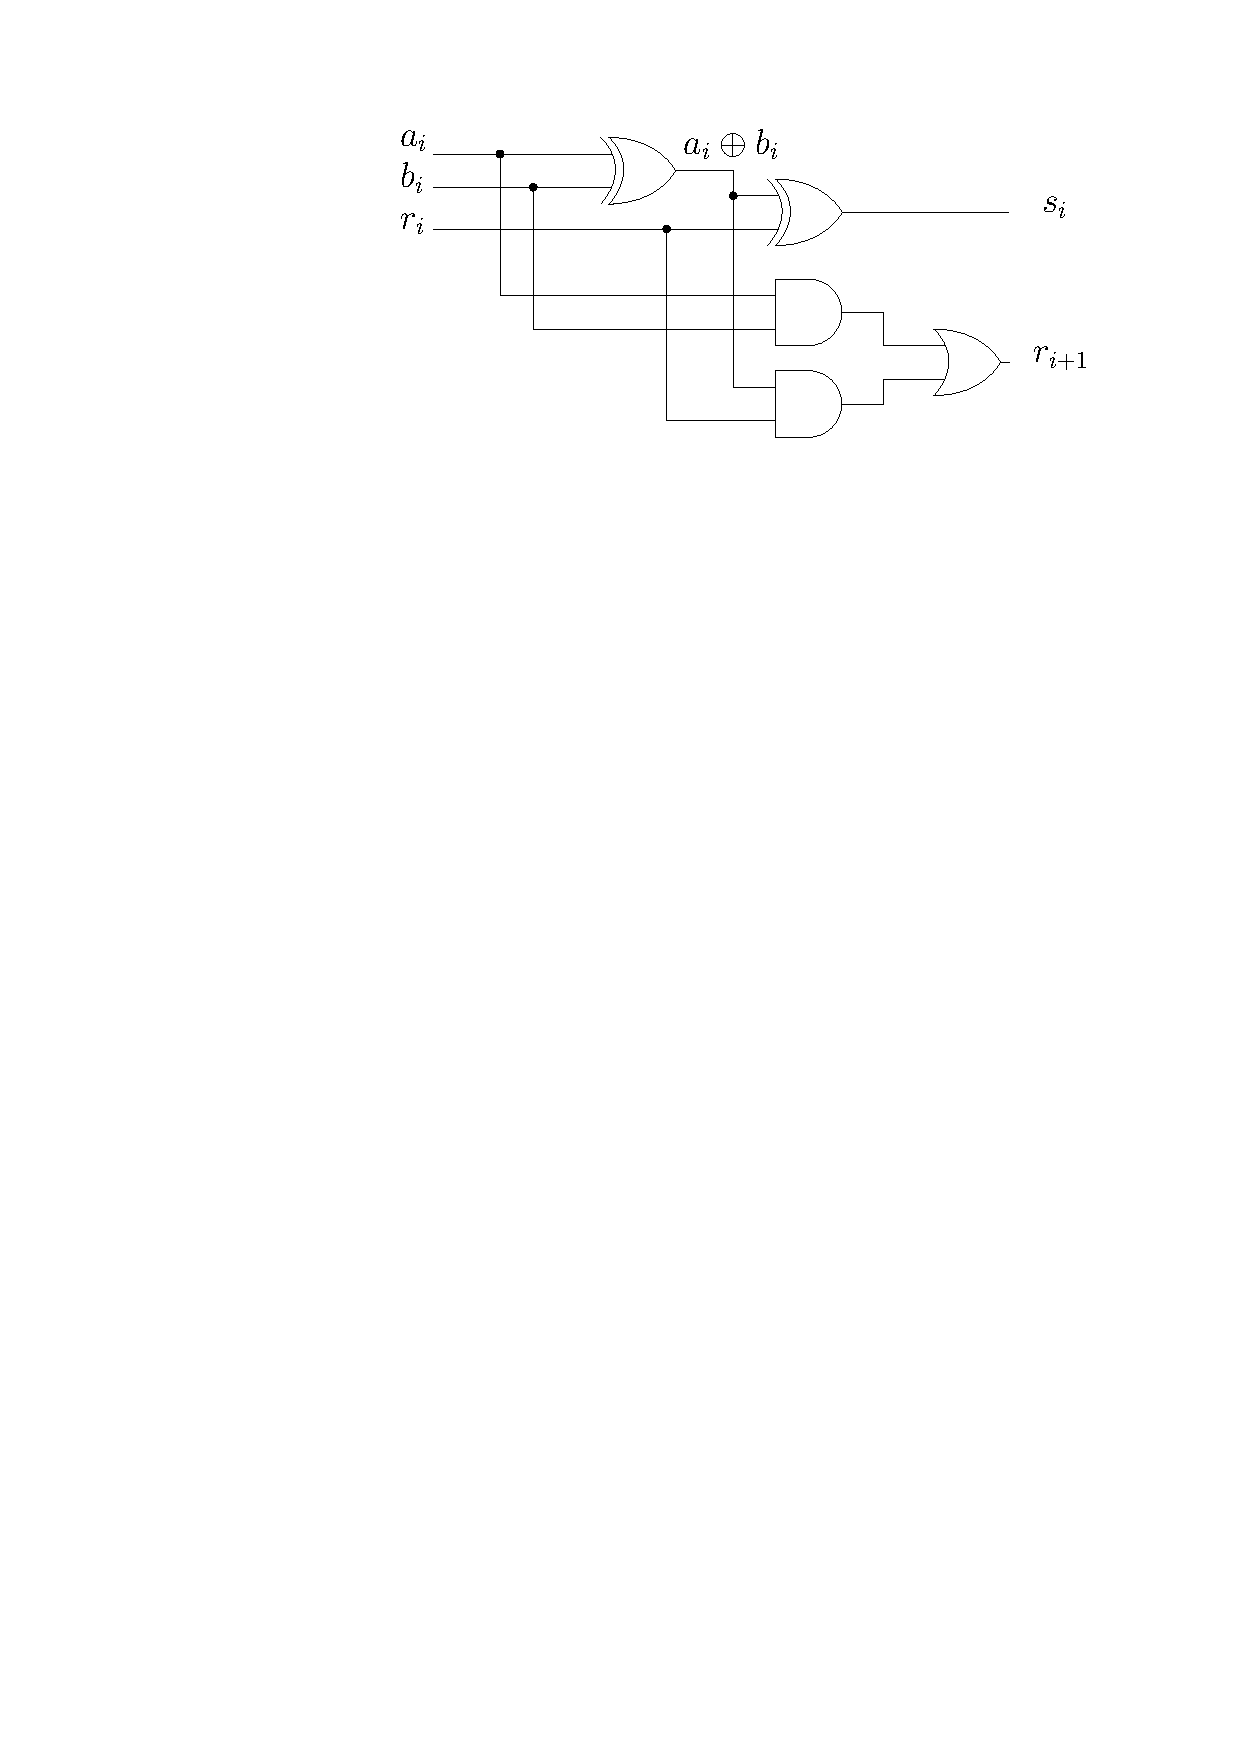
\includegraphics[width=\columnwidth]{Figs/adder.pdf}\\\centering b)
   \end{minipage}

\end{block}
\end{frame}


\begin{frame}
\frametitle{Unité arithmétique et logique (UAL) - Additionneur}
\begin{block}{Additionneur n bits}
\centering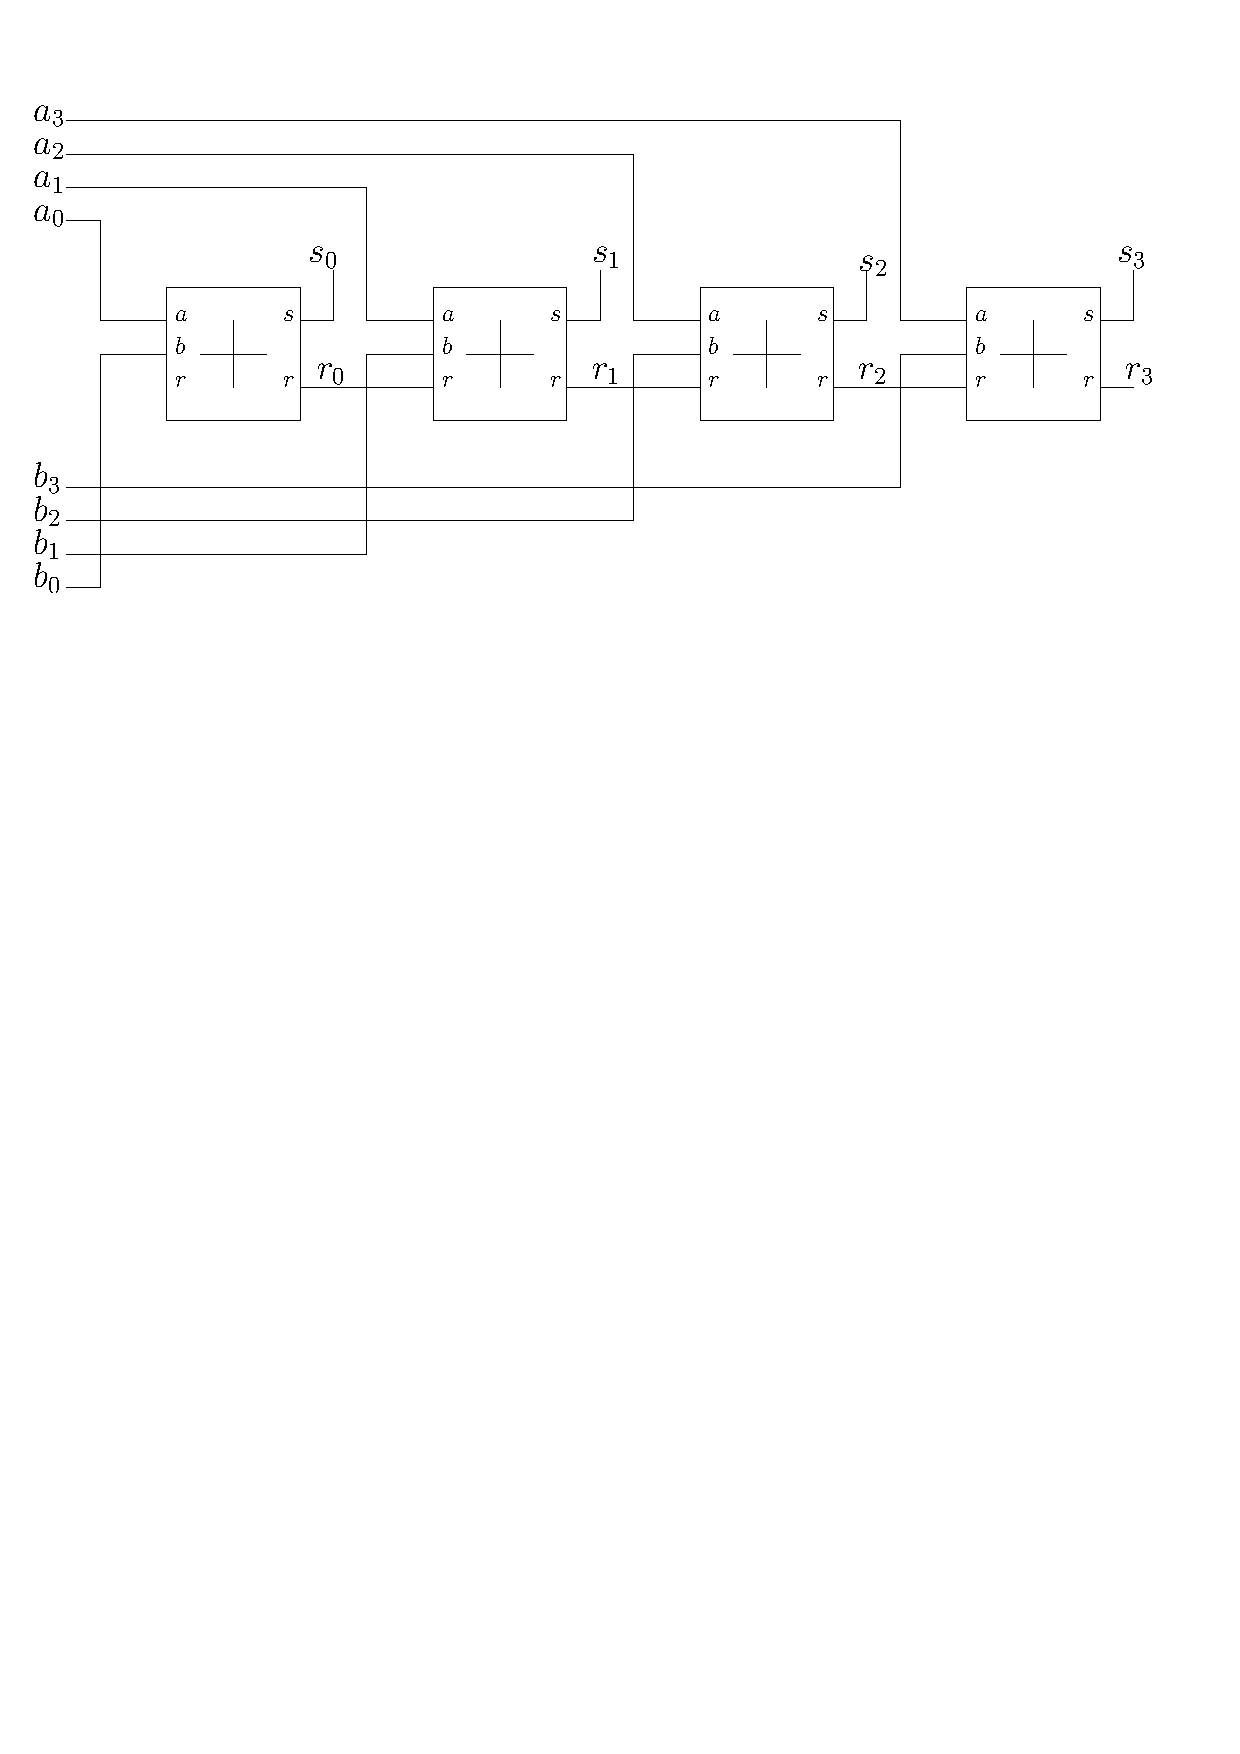
\includegraphics[width=0.75\linewidth]{Figs/adder_n.pdf}
\end{block}
\end{frame}

\begin{frame}
\frametitle{Unité arithmétique et logique (UAL)}
\begin{block}{Synthèse de l'UAL}
\begin{itemize}
\item on réalise chacun des circuits opératoires
\item on les combine et sélectionne grâce à un décodeur
\end{itemize}

   \begin{minipage}[c]{.4\linewidth}
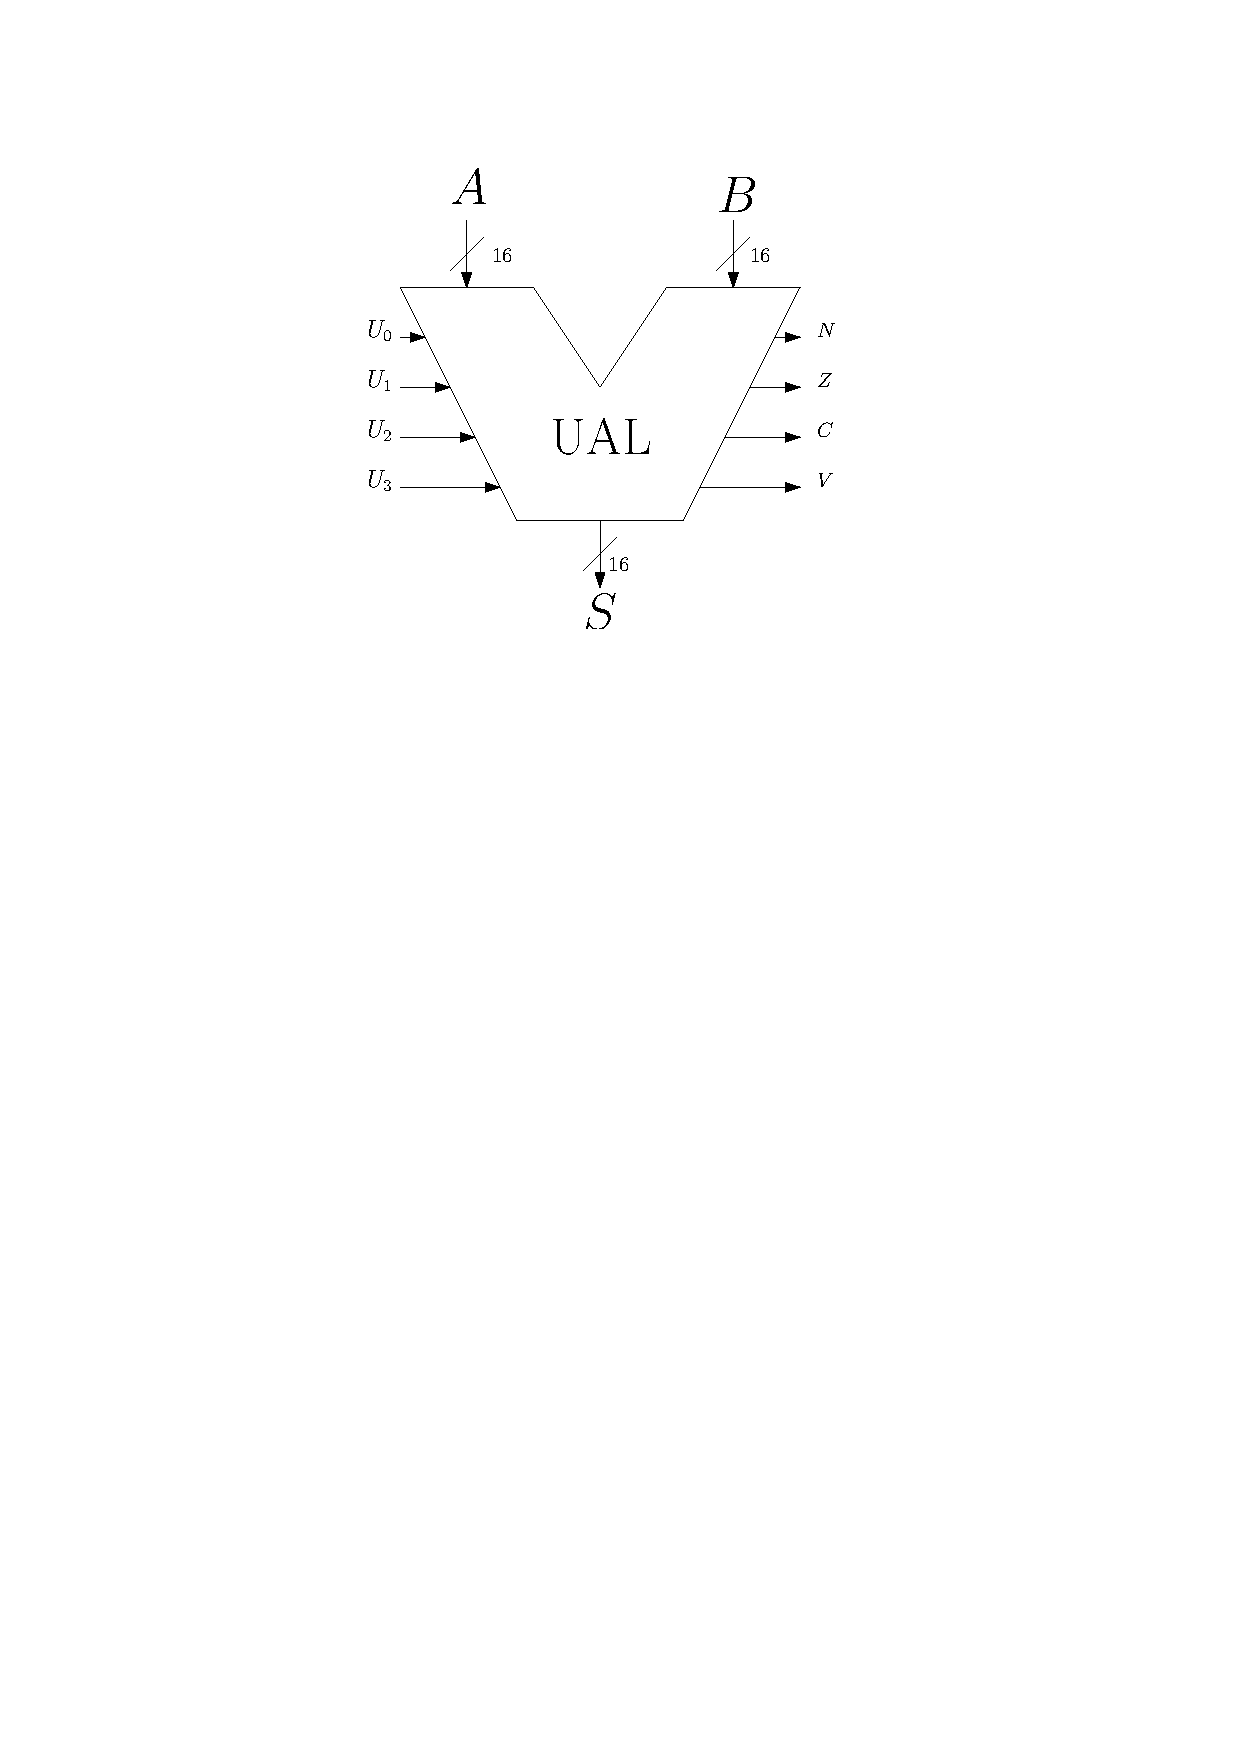
\includegraphics[width=\linewidth]{Figs/ual.pdf}\\\centering a)
   \end{minipage} \hfill
   \begin{minipage}[c]{.58\linewidth}
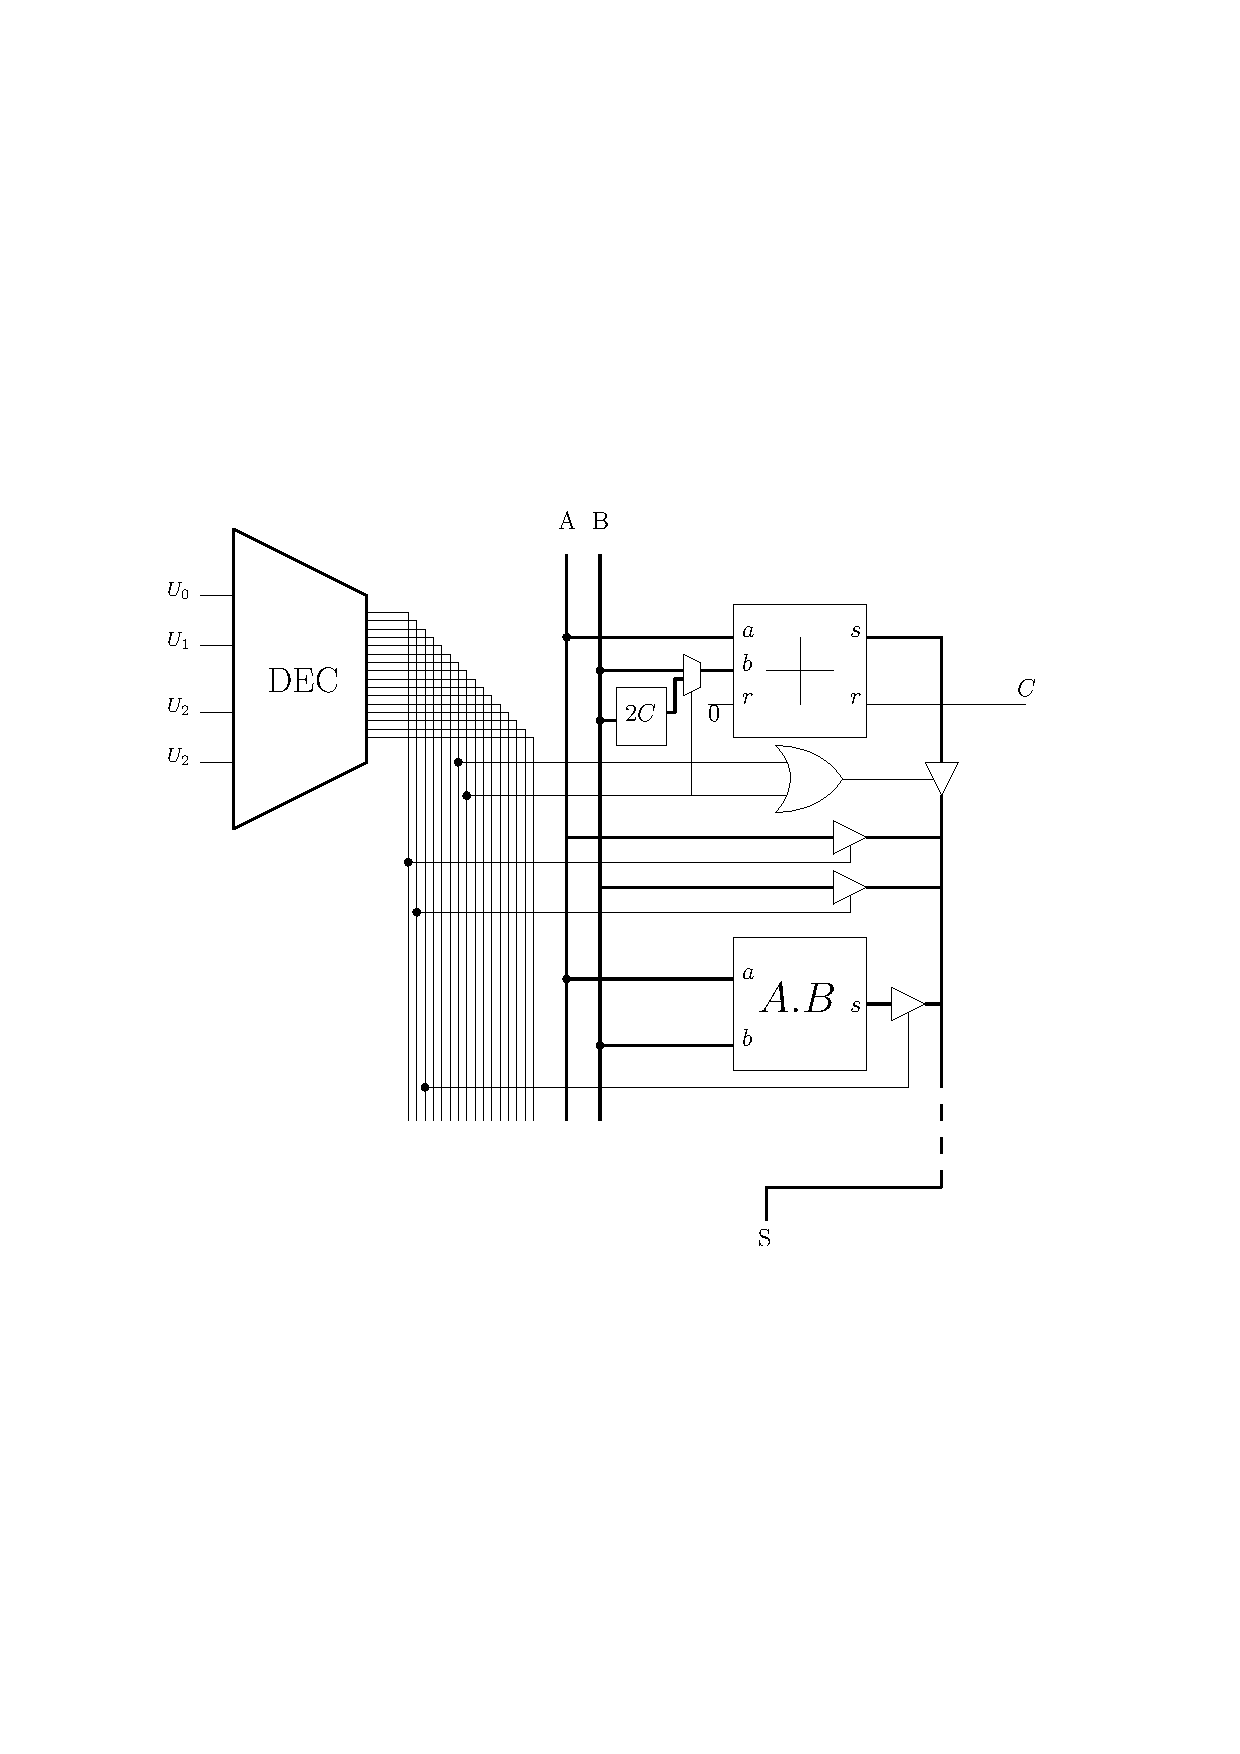
\includegraphics[width=\columnwidth]{Figs/ual_inner.pdf}\\\centering b)
   \end{minipage}

\end{block}
\end{frame}

\subsection{Résumons}
\begin{frame}
\frametitle{Résumons}
\begin{small}
\begin{block}{Logique combinatoire}
Pour réaliser un circuit de logique combinatoire 
\begin{itemize}
\item spécification fonctionnelle : table de vérité, équation logique
\item simplification de l'équation (e.g. tableaux de karnaugh)
\item circuit avec les portes logiques ET, OU, NOT (ou juste NAND, NOR, MUX)
\end{itemize}
\end{block}
\end{small}
\begin{block}{Par exemple}
\centering\includegraphics[width=\linewidth]{Figs/circuits_logique_combinatoire.pdf}
\end{block}
\end{frame}

\begin{frame}
\frametitle{C'est tout ?}
Problème : un bouton (0/1) - une lumière (0/1)
\begin{block}{Allumons}
\centering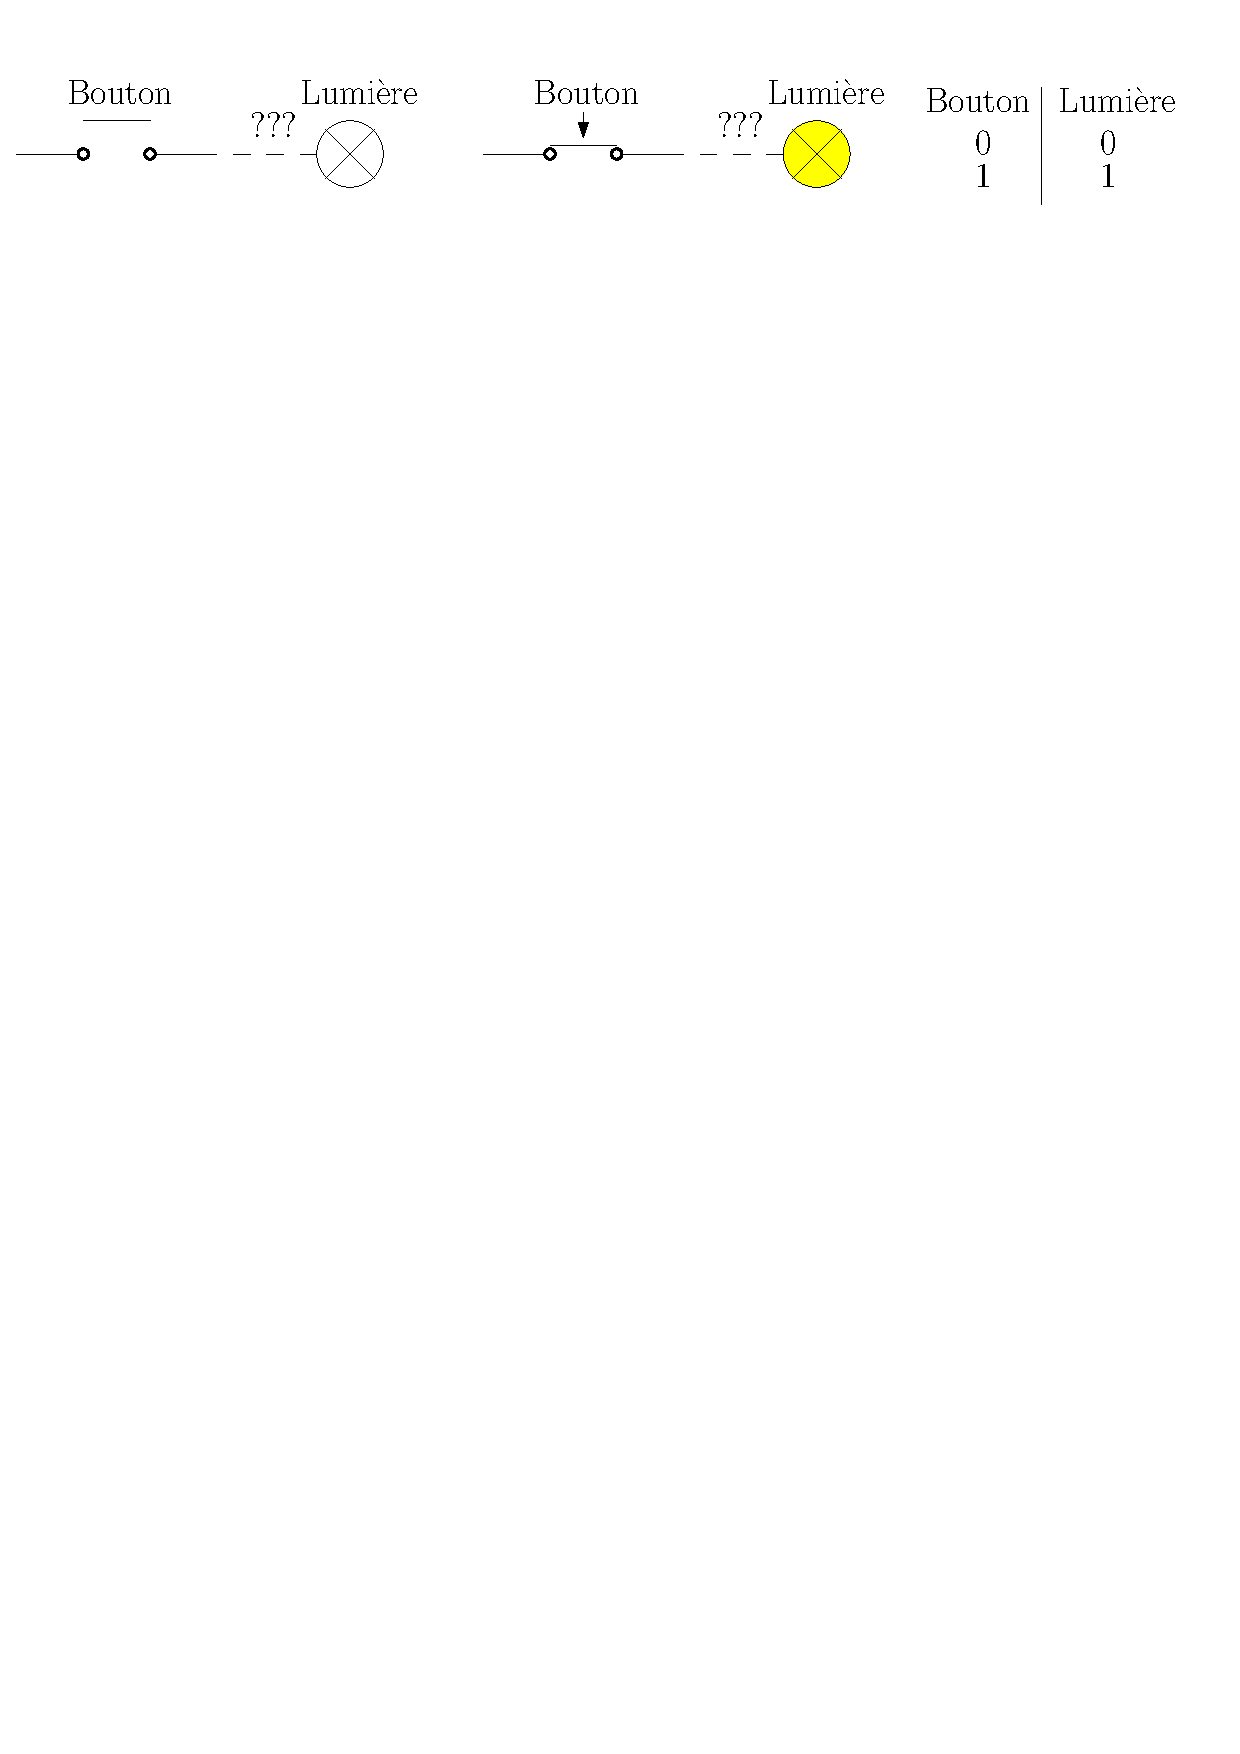
\includegraphics[width=\linewidth]{Figs/bouton_lumiere1.pdf}
\end{block}
\begin{block}{Eteignons}
\centering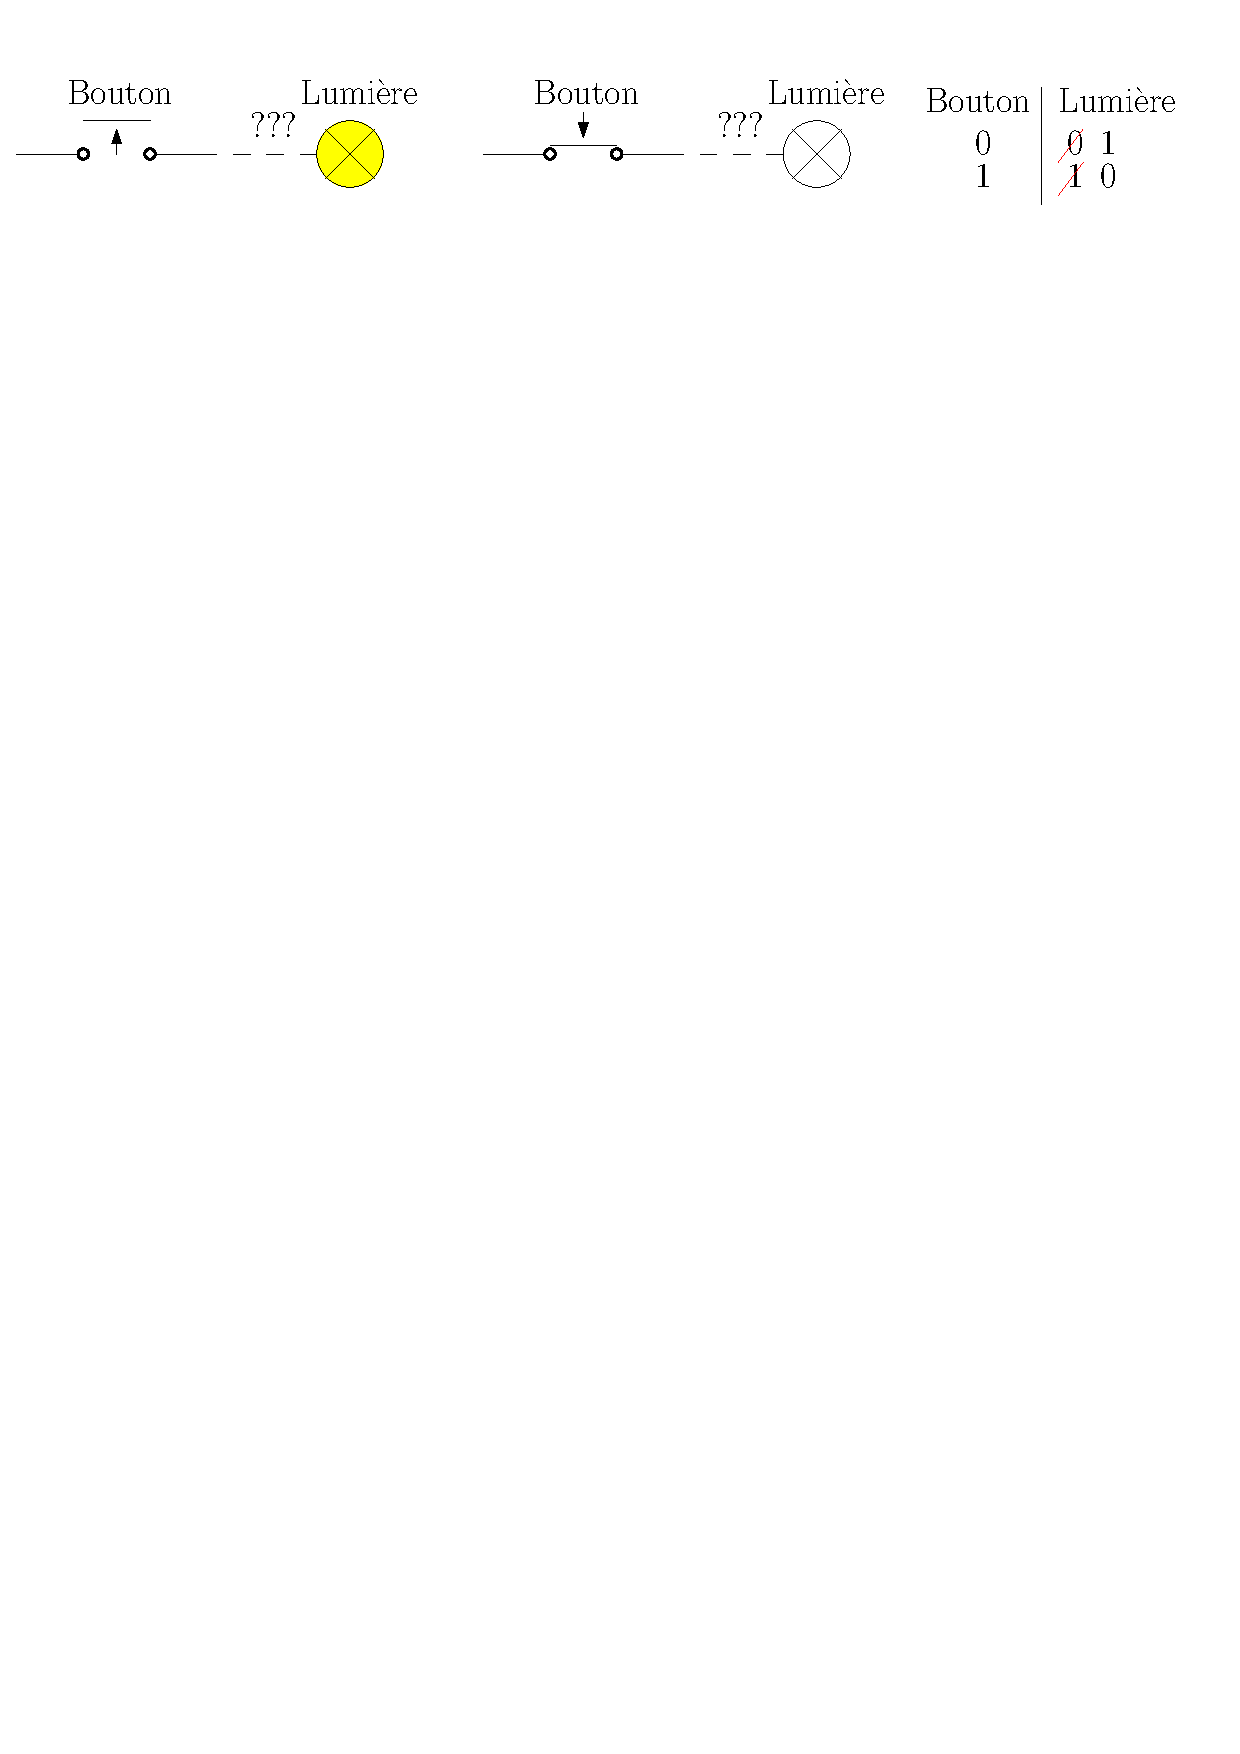
\includegraphics[width=\linewidth]{Figs/bouton_lumiere2.pdf}
\end{block}
$\Rightarrow$ mince ?!?!
\end{frame}

\begin{frame}
\frametitle{C'est tout ?}
Problème : un bouton (0/1) - une lumière (0/1)
\begin{block}{Solution}
\centering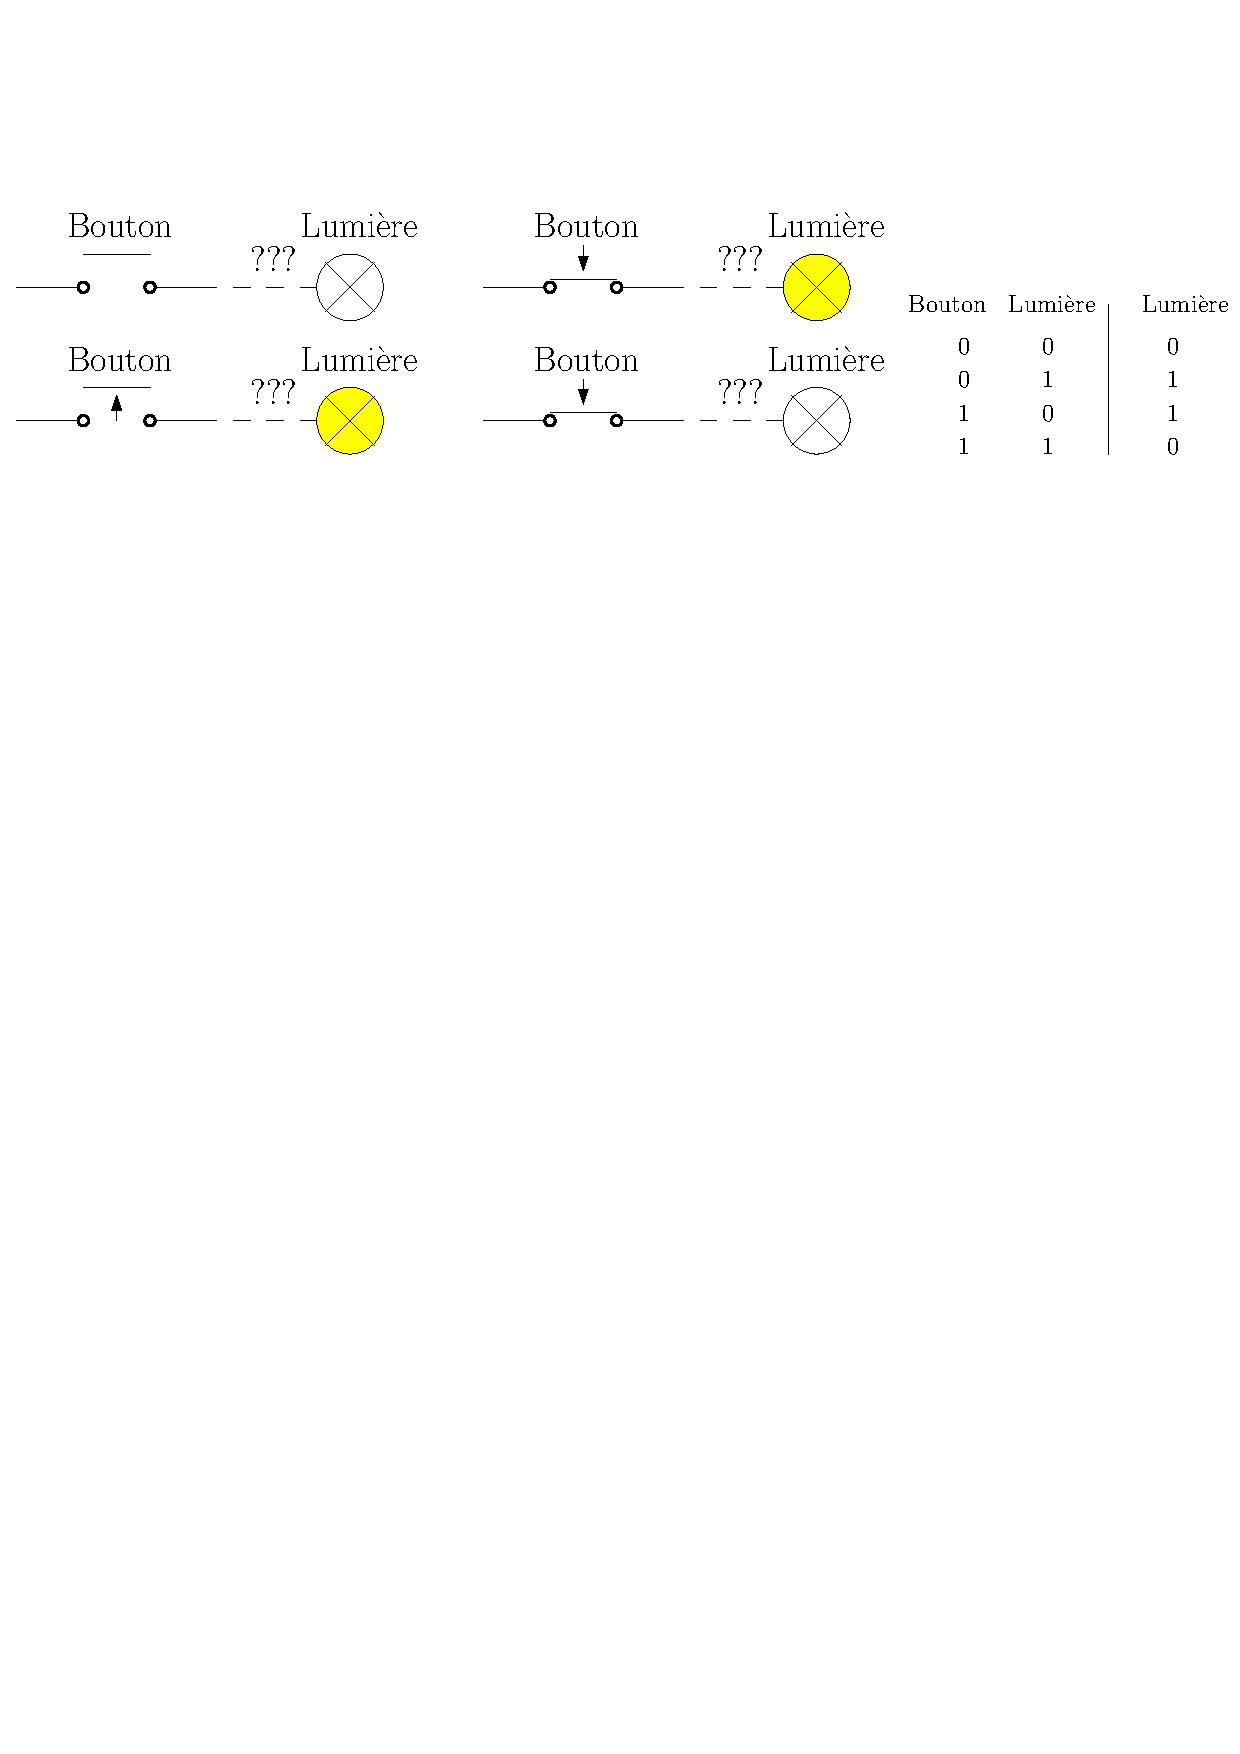
\includegraphics[width=\linewidth]{Figs/bouton_lumiere.pdf}
\end{block}
Le \textbf{nouvel état} lumière dépends de l'\textbf{entrée bouton} et de l'\textbf{ancien état} lumière
\end{frame}

\begin{frame}
\frametitle{Plus généralement}
\begin{block}{On reboucle simplement la sortie sur l'entrée ?}
Ce n'est pas forcément la sortie qui est utilisée en entrée puisque je peux très bien avoir besoin de produire la même sortie dans des états différents
%\textcolor{red}{HORLOGE ??}
\end{block}
\end{frame}

%%%%%%%%%%%%%%%%%%%%%%%%%%%%
\subsection{Logique séquentielle}

\begin{frame}
\frametitle{Logique séquentielle}

\begin{block}{Transducteur fini}
\vspace{1cm}
%\textcolor{red}{Machine à état fini pour le pb du bouton/lampe}
\centering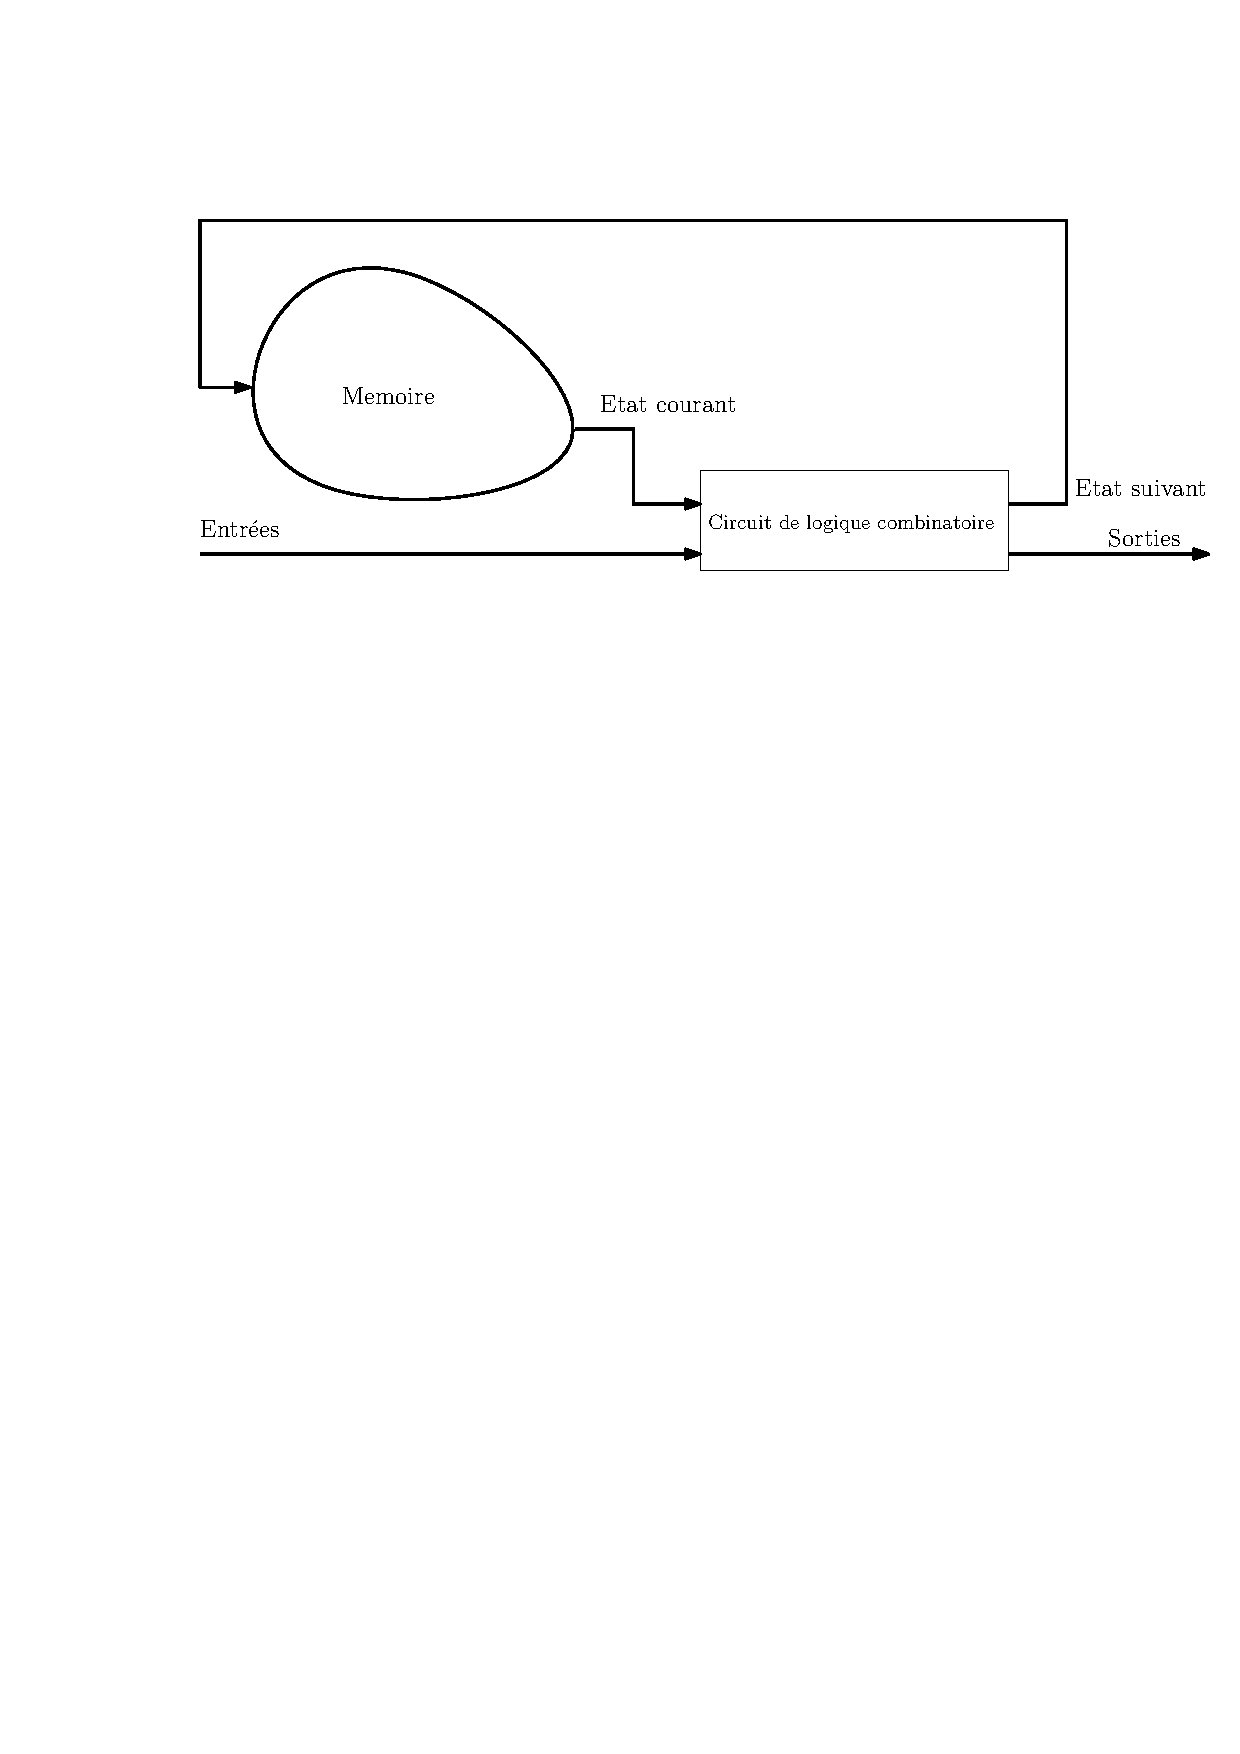
\includegraphics[width=\linewidth]{Figs/intro_seq.pdf}
\vspace{1cm}
\end{block}

\end{frame}

\begin{frame}
\frametitle{Verrou Reset-Set (RS)}

\begin{block}{Schéma et Chronogramme}
\begin{minipage}[c]{0.25\columnwidth}
\tikzstyle{branch}=[fill,shape=circle,minimum size=3pt,inner sep=0pt]
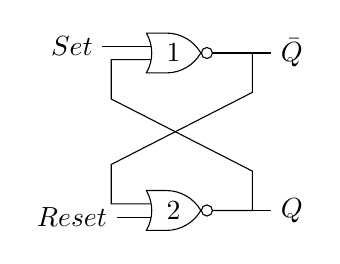
\begin{tikzpicture}[label distance=2mm]

    \node[nor gate US, draw, logic gate inputs=nn] at (0,0) (Nor1) {};
    \node[nor gate US, draw, logic gate inputs=nn] at (0,-2) (Nor2) {};

    \node (S) at ($(Nor1.input 1) - (1,0)$) {$Set$};
    \node (R) at ($(Nor2.input 2) - (1,0)$) {$Reset$};
    \node (bQ) at ($(Nor1.output) + (1, 0)$) {$\bar{Q}$};
    \node (Q) at ($(Nor2.output) + (1, 0)$) {$Q$};

    \node at ($(Nor1.output) - (0.5,0)$) {$1$};
    \node at ($(Nor2.output) - (0.5,0)$) {$2$};

    \draw (S) -- (Nor1.input 1);
    \draw (Nor2.output) -- ([xshift=0.5cm]Nor2.output) -- ++(0, 0.5) -- ([xshift=-0.5cm,yshift=-0.5cm]Nor1.input 2) -- ([xshift=-0.5cm]Nor1.input 2) -- (Nor1.input 2);
    \draw (Nor1.output) -- (bQ);

    \draw (R) -- (Nor2.input 2);
    \draw (Nor1.output) -- ([xshift=0.5cm]Nor1.output) -- ++(0, -0.5) -- ([xshift=-0.5cm,yshift=+0.5cm]Nor2.input 1) -- ([xshift=-0.5cm]Nor2.input 1) -- (Nor2.input 1);
    \draw (Nor2.output) -- (Q);
\end{tikzpicture}
\end{minipage}
\hspace{2cm}
\begin{minipage}[c]{0.5\columnwidth}
\begin{tikztimingtable}[
    timing/coldist=2pt,     % column distance
    xscale=0.75,yscale=1, % scale diagrams
    semithick               % set line width
]
$R$       & 2L       LLLLLL       LLLLLL       HHHHHH       LLLLLL  \\
$S$       & 2L       HHHHHH       LLLLLL       LLLLLL       LLLLLL  \\
$Q$       & 2L       LLHHHH       HHHHHH       HLLLLL       LLLLLL\\
$\bar{Q}$ & 2H N(Q1) HLLLLL N(Q2) LLLLLL N(Q3) LLHHHH N(Q4) HHHHHH \\
          & SS       SSSSSS       SSSSSS       SSSSSS       SSSSSS\\
\extracode
  %\tablerules
  %\tablegrid
  \begin{pgfonlayer}{background}
    \vertlines[help  lines]{2,4,8,14,16,20}
    \draw[thick,<->,shorten >=2pt,shorten <=2pt,>=stealth] (2, -8) -- (4,-8);
    \draw [anchor=mid] node at (3,-7) {\tiny $\Delta$};
    \draw [anchor=north] let \p1=(Q1) in node at (\x1,-9) {$t_0$};

    \draw [anchor=north] let \p1=(Q2) in node at (\x1,-9) {$t_1$};

    \draw[thick,<->,shorten >=2pt,shorten <=2pt,>=stealth] (14, -8) -- (16,-8);
    \draw [anchor=mid] node at (15,-7) {\tiny $\Delta$};
    \draw [anchor=north] let \p1=(Q3) in node at (\x1,-9) {$t_2$};

    \draw [anchor=north] let \p1=(Q4) in node at (\x1,-9) {$t_3$};
  \end{pgfonlayer}
\end{tikztimingtable}
\end{minipage}
\end{block}
$\Rightarrow$ effet mémoire si R=S=0 ($t_1 \leq t \leq t_2$, $t \geq t_3$)
\end{frame}

\begin{frame}
\frametitle{En fait ... c'est plus compliqué}
\begin{block}{Machine à états finis pour un circuit symétrique}
\begin{minipage}[c]{0.25\columnwidth}
\tikzstyle{branch}=[fill,shape=circle,minimum size=3pt,inner sep=0pt]
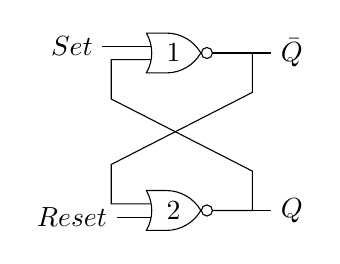
\begin{tikzpicture}[label distance=2mm]

    \node[nor gate US, draw, logic gate inputs=nn] at (0,0) (Nor1) {};
    \node[nor gate US, draw, logic gate inputs=nn] at (0,-2) (Nor2) {};

    \node (S) at ($(Nor1.input 1) - (1,0)$) {$Set$};
    \node (R) at ($(Nor2.input 2) - (1,0)$) {$Reset$};
    \node (bQ) at ($(Nor1.output) + (1, 0)$) {$\bar{Q}$};
    \node (Q) at ($(Nor2.output) + (1, 0)$) {$Q$};

    \node at ($(Nor1.output) - (0.5,0)$) {$1$};
    \node at ($(Nor2.output) - (0.5,0)$) {$2$};

    \draw (S) -- (Nor1.input 1);
    \draw (Nor2.output) -- ([xshift=0.5cm]Nor2.output) -- ++(0, 0.5) -- ([xshift=-0.5cm,yshift=-0.5cm]Nor1.input 2) -- ([xshift=-0.5cm]Nor1.input 2) -- (Nor1.input 2);
    \draw (Nor1.output) -- (bQ);

    \draw (R) -- (Nor2.input 2);
    \draw (Nor1.output) -- ([xshift=0.5cm]Nor1.output) -- ++(0, -0.5) -- ([xshift=-0.5cm,yshift=+0.5cm]Nor2.input 1) -- ([xshift=-0.5cm]Nor2.input 1) -- (Nor2.input 1);
    \draw (Nor2.output) -- (Q);
\end{tikzpicture}
\end{minipage}
\hspace{1cm}
\begin{minipage}[c]{0.5\columnwidth}
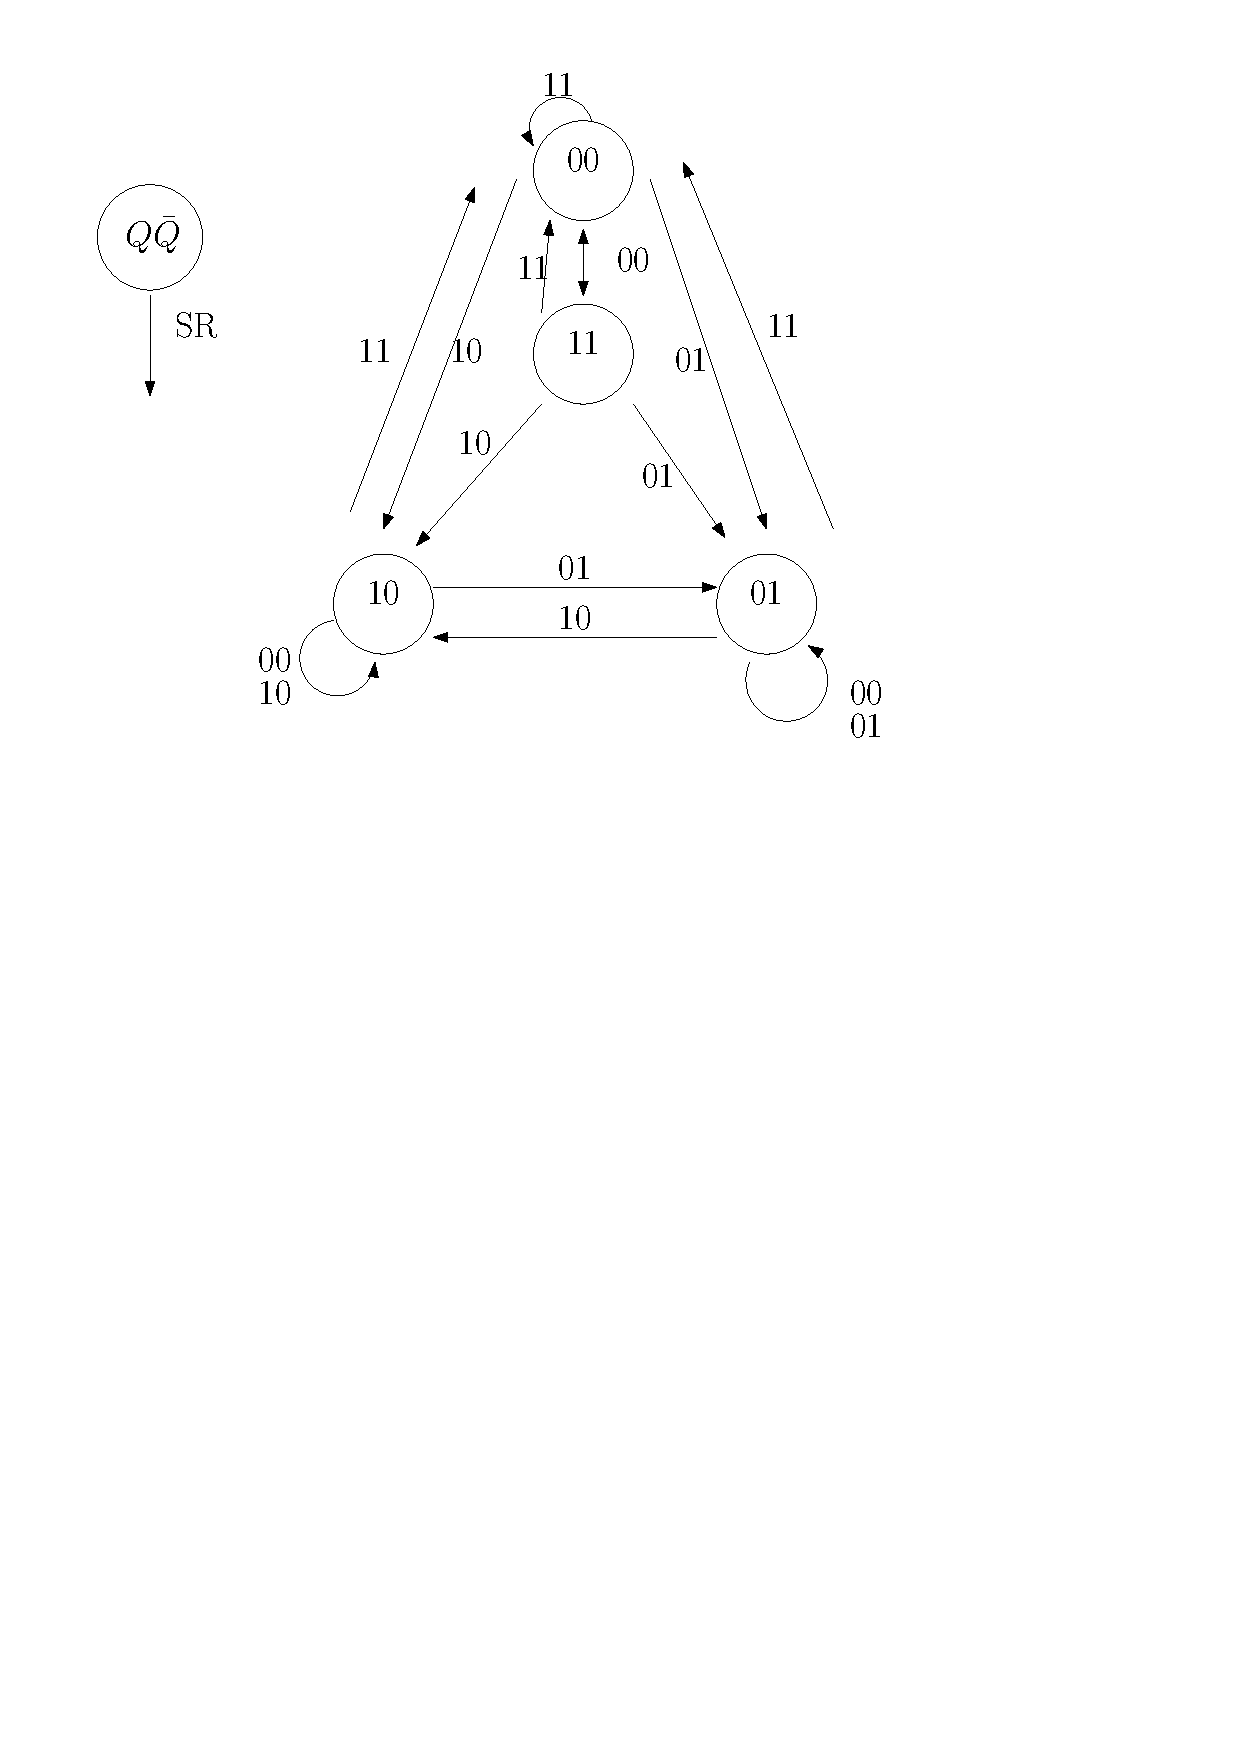
\includegraphics[width=\columnwidth]{Figs/RS_fsm.pdf}
\end{minipage}
$\Rightarrow$ logique synchrone et logique asynchrone
\end{block}
\end{frame}

\begin{frame}
\frametitle{Supprimer les états instables}
\begin{block}{Et si $R.S = 0$ ?}
\begin{minipage}[c]{0.25\columnwidth}
\tikzstyle{branch}=[fill,shape=circle,minimum size=3pt,inner sep=0pt]
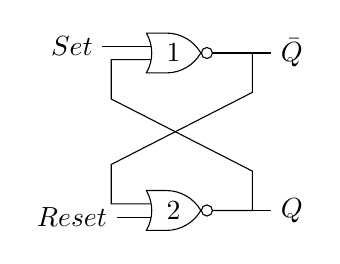
\begin{tikzpicture}[label distance=2mm]

    \node[nor gate US, draw, logic gate inputs=nn] at (0,0) (Nor1) {};
    \node[nor gate US, draw, logic gate inputs=nn] at (0,-2) (Nor2) {};

    \node (S) at ($(Nor1.input 1) - (1,0)$) {$Set$};
    \node (R) at ($(Nor2.input 2) - (1,0)$) {$Reset$};
    \node (bQ) at ($(Nor1.output) + (1, 0)$) {$\bar{Q}$};
    \node (Q) at ($(Nor2.output) + (1, 0)$) {$Q$};

    \node at ($(Nor1.output) - (0.5,0)$) {$1$};
    \node at ($(Nor2.output) - (0.5,0)$) {$2$};

    \draw (S) -- (Nor1.input 1);
    \draw (Nor2.output) -- ([xshift=0.5cm]Nor2.output) -- ++(0, 0.5) -- ([xshift=-0.5cm,yshift=-0.5cm]Nor1.input 2) -- ([xshift=-0.5cm]Nor1.input 2) -- (Nor1.input 2);
    \draw (Nor1.output) -- (bQ);

    \draw (R) -- (Nor2.input 2);
    \draw (Nor1.output) -- ([xshift=0.5cm]Nor1.output) -- ++(0, -0.5) -- ([xshift=-0.5cm,yshift=+0.5cm]Nor2.input 1) -- ([xshift=-0.5cm]Nor2.input 1) -- (Nor2.input 1);
    \draw (Nor2.output) -- (Q);
\end{tikzpicture}
\end{minipage}
\hspace{1cm}
\begin{minipage}[c]{0.5\columnwidth}
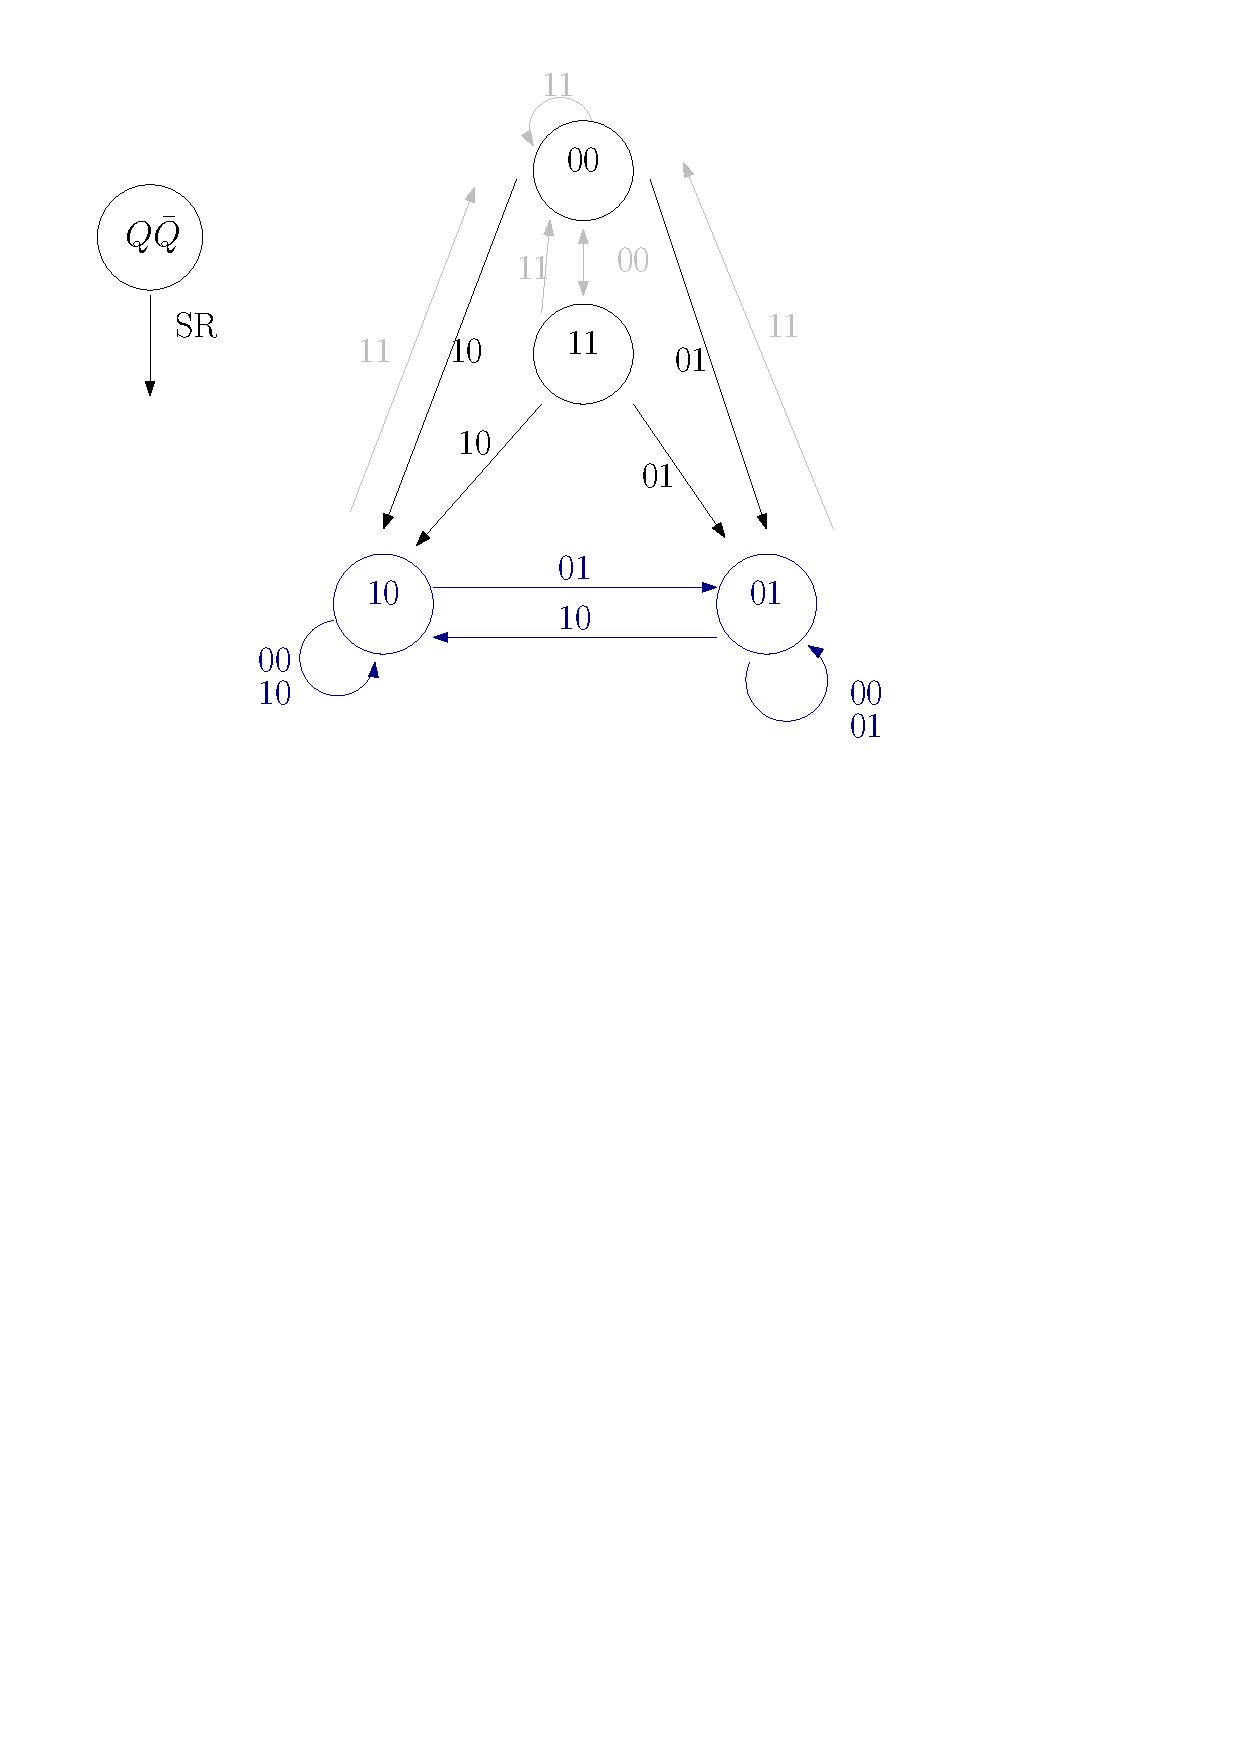
\includegraphics[width=\columnwidth]{Figs/RS_fsm_comp.pdf}
\end{minipage}
\end{block}
\end{frame}

\begin{frame}
\frametitle{Mémoriser un bit sur niveau haut : Verrou D}
\begin{block}{Schéma et chronogramme}

  \begin{minipage}[c]{.7\linewidth}
\tikzstyle{branch}=[fill,shape=circle,minimum size=3pt,inner sep=0pt]
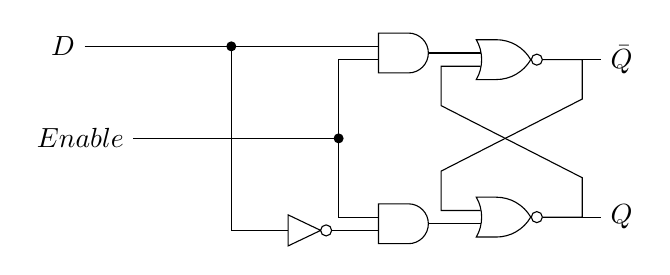
\begin{tikzpicture}[label distance=2mm]

    \node[nor gate US, draw, logic gate inputs=nn] at (0,0) (Nor1) {};
    \node[nor gate US, draw, logic gate inputs=nn] at (0,-2) (Nor2) {};
    \node[and gate US, draw, logic gate inputs=nn] at ($(Nor1.input 1) - (1, 0)$) (And1) {};
    \node[and gate US, draw, logic gate inputs=nn] at ($(Nor2.input 2) - (1, 0)$) (And2) {};
    \node[not gate US, draw] at ($(And2.input 2) - (1,0)$) (Not) {};

    \node (D) at ($(And1.input 1) - (4,0)$) {$D$};

    \node[right] (E) at (-6,-1) {$Enable$};
    \node (bQ) at ($(Nor1.output) + (1, 0)$) {$\bar{Q}$};
    \node (Q) at ($(Nor2.output) + (1, 0)$) {$Q$};

    \node at ($(Nor1.output) - (0.5,0)$) {};
    \node at ($(Nor2.output) - (0.5,0)$) {};

    \draw (D) -- (And1.input 1) node [midway,circ] (S) {};
    \draw (S) |- (Not.input);

    \draw (And1.output) -- (Nor1.input 1);
    \draw (Not.output) -- (And2.input 2);
    \draw (And2.output) -- (Nor2.input 2);
    \draw (E) -| ($(And1.input 2)-(0.5,0)$) node[midway,circ]{} -- (And1.input 2);
    \draw (E) -| ($(And2.input 1)-(0.5,0)$) -- (And2.input 1);



    \draw (Nor2.output) -- ([xshift=0.5cm]Nor2.output) -- ++(0, 0.5) -- ([xshift=-0.5cm,yshift=-0.5cm]Nor1.input 2) -- ([xshift=-0.5cm]Nor1.input 2) -- (Nor1.input 2);
    \draw (Nor1.output) -- (bQ);

    \draw (Nor1.output) -- ([xshift=0.5cm]Nor1.output) -- ++(0, -0.5) -- ([xshift=-0.5cm,yshift=+0.5cm]Nor2.input 1) -- ([xshift=-0.5cm]Nor2.input 1) -- (Nor2.input 1);
    \draw (Nor2.output) -- (Q);
\end{tikzpicture}\\
\end{minipage}\hfill
\begin{minipage}[c]{.2\linewidth}
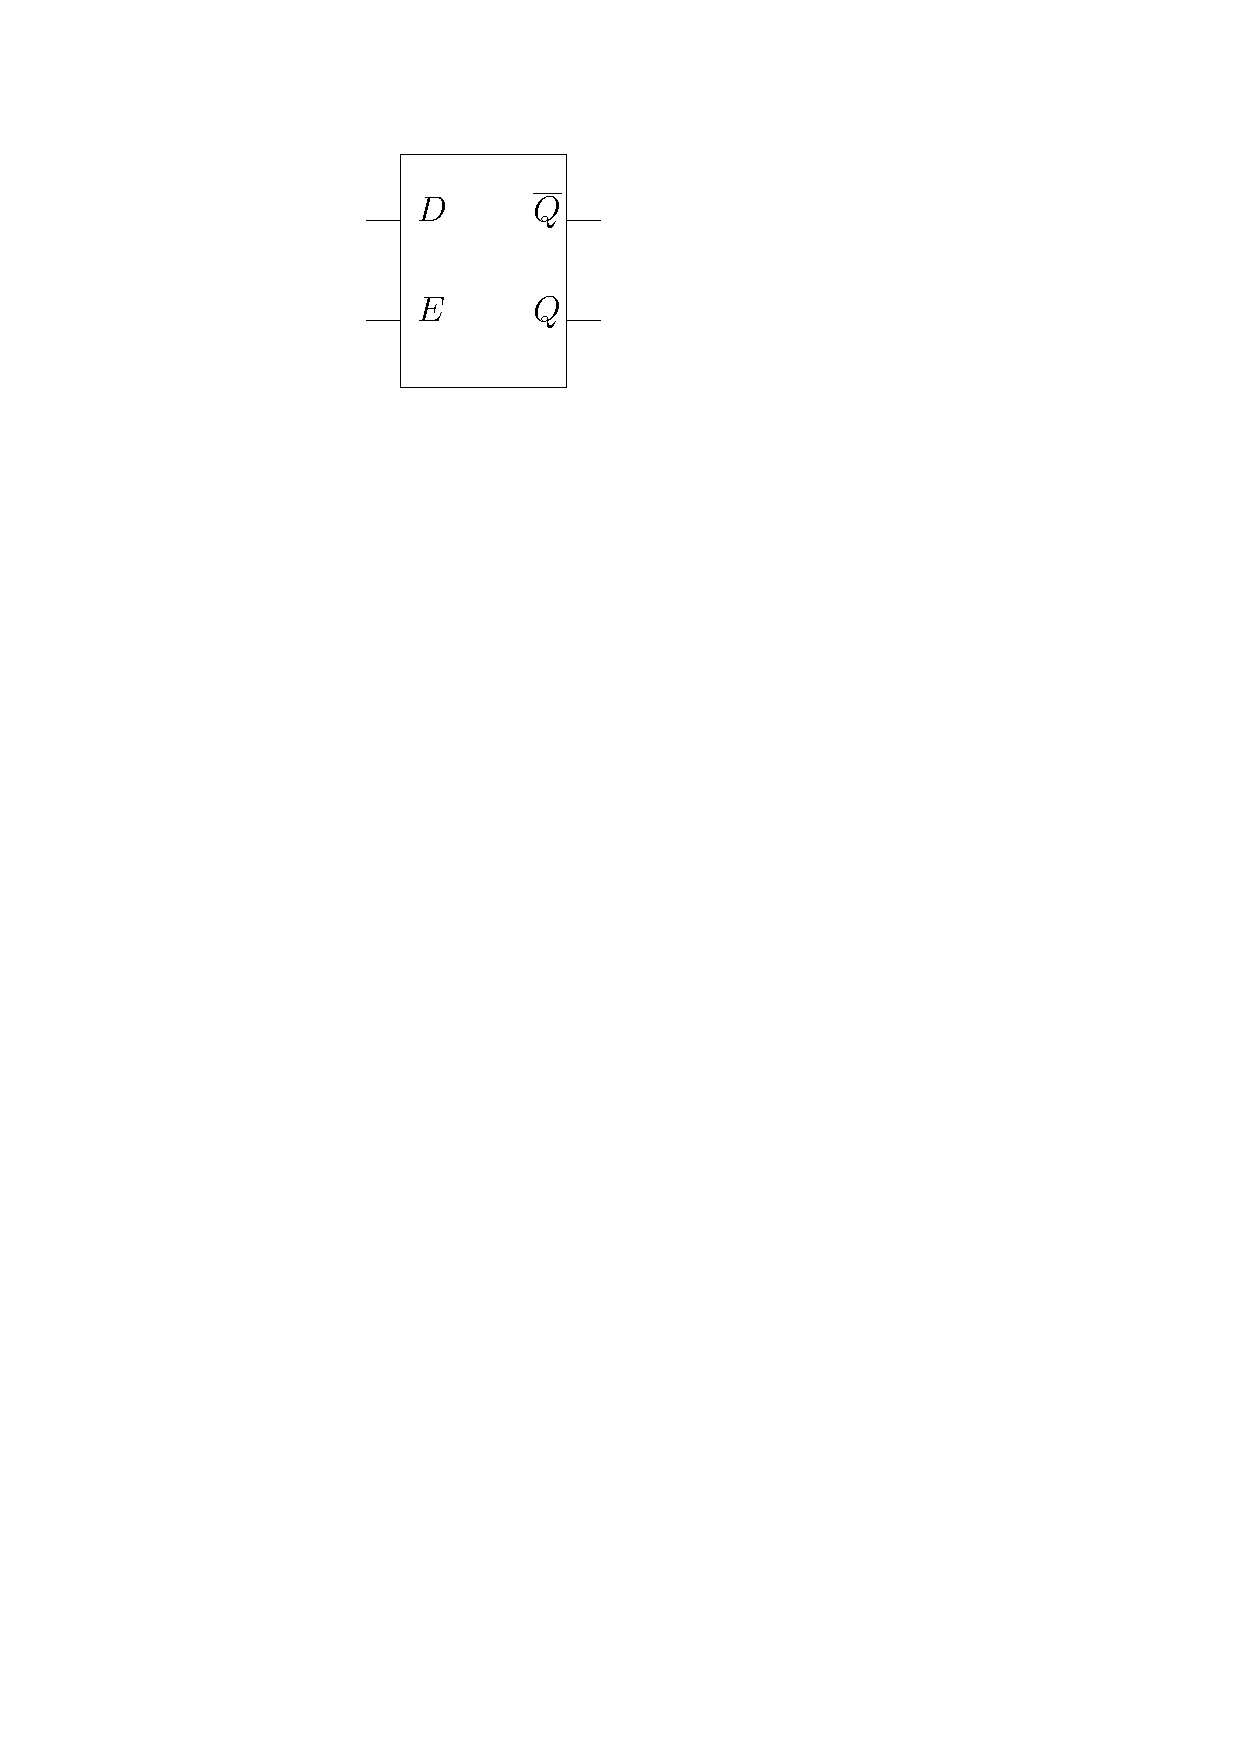
\includegraphics[width=\columnwidth]{Figs/verrou_D.pdf}
\end{minipage}


\begin{framed}
\begin{itemize}
\item $Set = D . Enable$
\item $Reset = \bar{D} . Enable$
\item $Q(t) = Enable.D + \overline{Enable}.Q(t-1)$
\end{itemize}
\end{framed}

\end{block}
\end{frame}


\begin{frame}
\frametitle{Mémoriser un bit sur niveau haut : Verrou D}
\begin{block}{Schéma et chronogramme}

\begin{minipage}[c]{.2\linewidth}
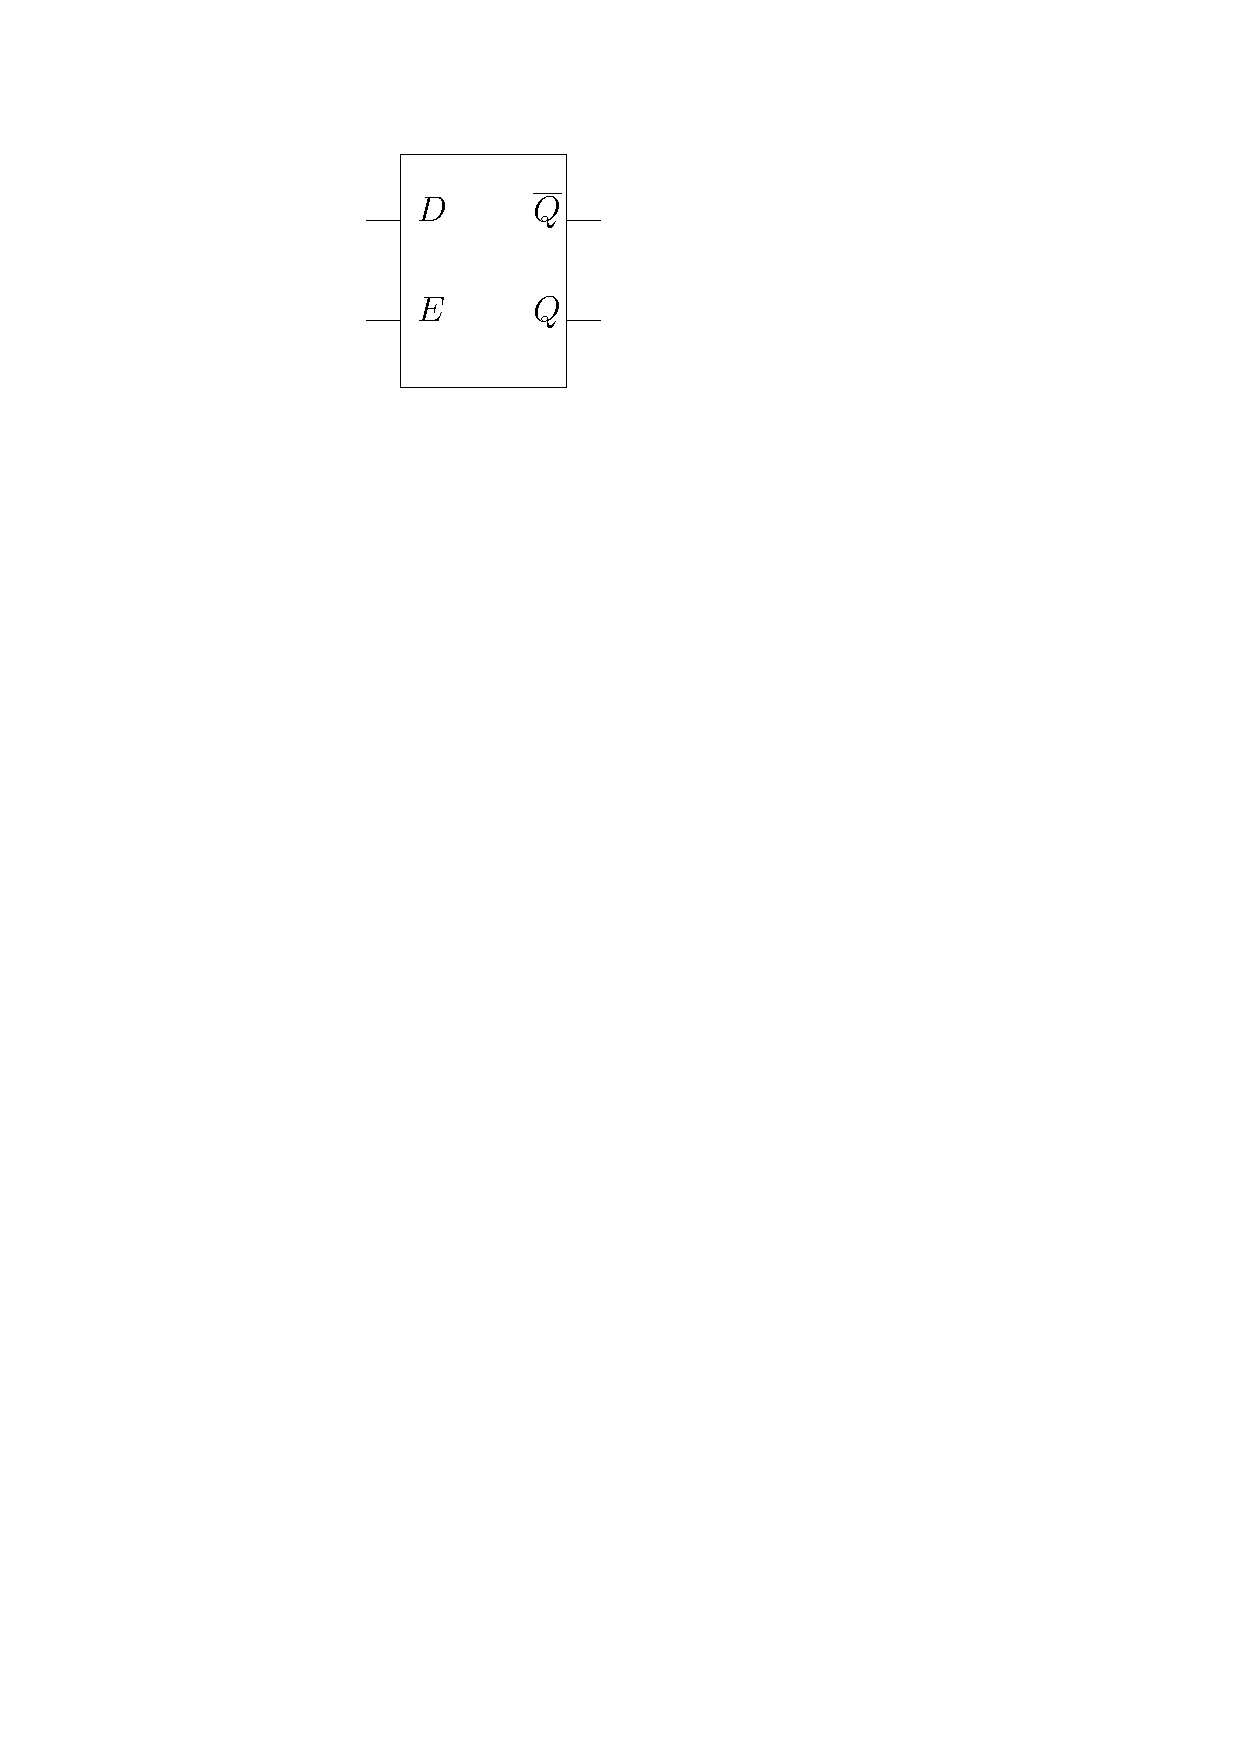
\includegraphics[width=\columnwidth]{Figs/verrou_D.pdf}
\end{minipage}
\hfill
  \begin{minipage}[c]{.7\linewidth}
\begin{tikztimingtable}[
    timing/coldist=2pt,     % column distance
    xscale=0.5,yscale=2, % scale diagrams
    semithick               % set line width
]
$Enable(Horloge)$ & 8L 8H 8L 8H \\
$D$       & 2L 3H 2L 2H  1L 2H 1L 1H 1L 3H  6L   2L 3H 3L \\
$Q$       & 8L 1H 1L 2H 1L 1H 1L 9H    2L 3H 3L\\
\extracode
  %\tablerules
  %\tablegrid
\end{tikztimingtable}
\end{minipage}

\begin{framed}
\begin{itemize}
\item $E=1 \Rightarrow Q = D$ : le verrou est transparent,
\item $E=0 \Rightarrow $ le verrou est dans un état mémoire, sa sortie ne change pas même si $D$ change
\end{itemize}
\end{framed}

\end{block}
\end{frame}


\begin{frame}
\frametitle{Mémoire sur front : Bascule D synchrone sur front montant}
\begin{block}{Bascule D : maître-esclave; Schéma et chronogramme}

\begin{minipage}[c]{0.4\linewidth}
\centering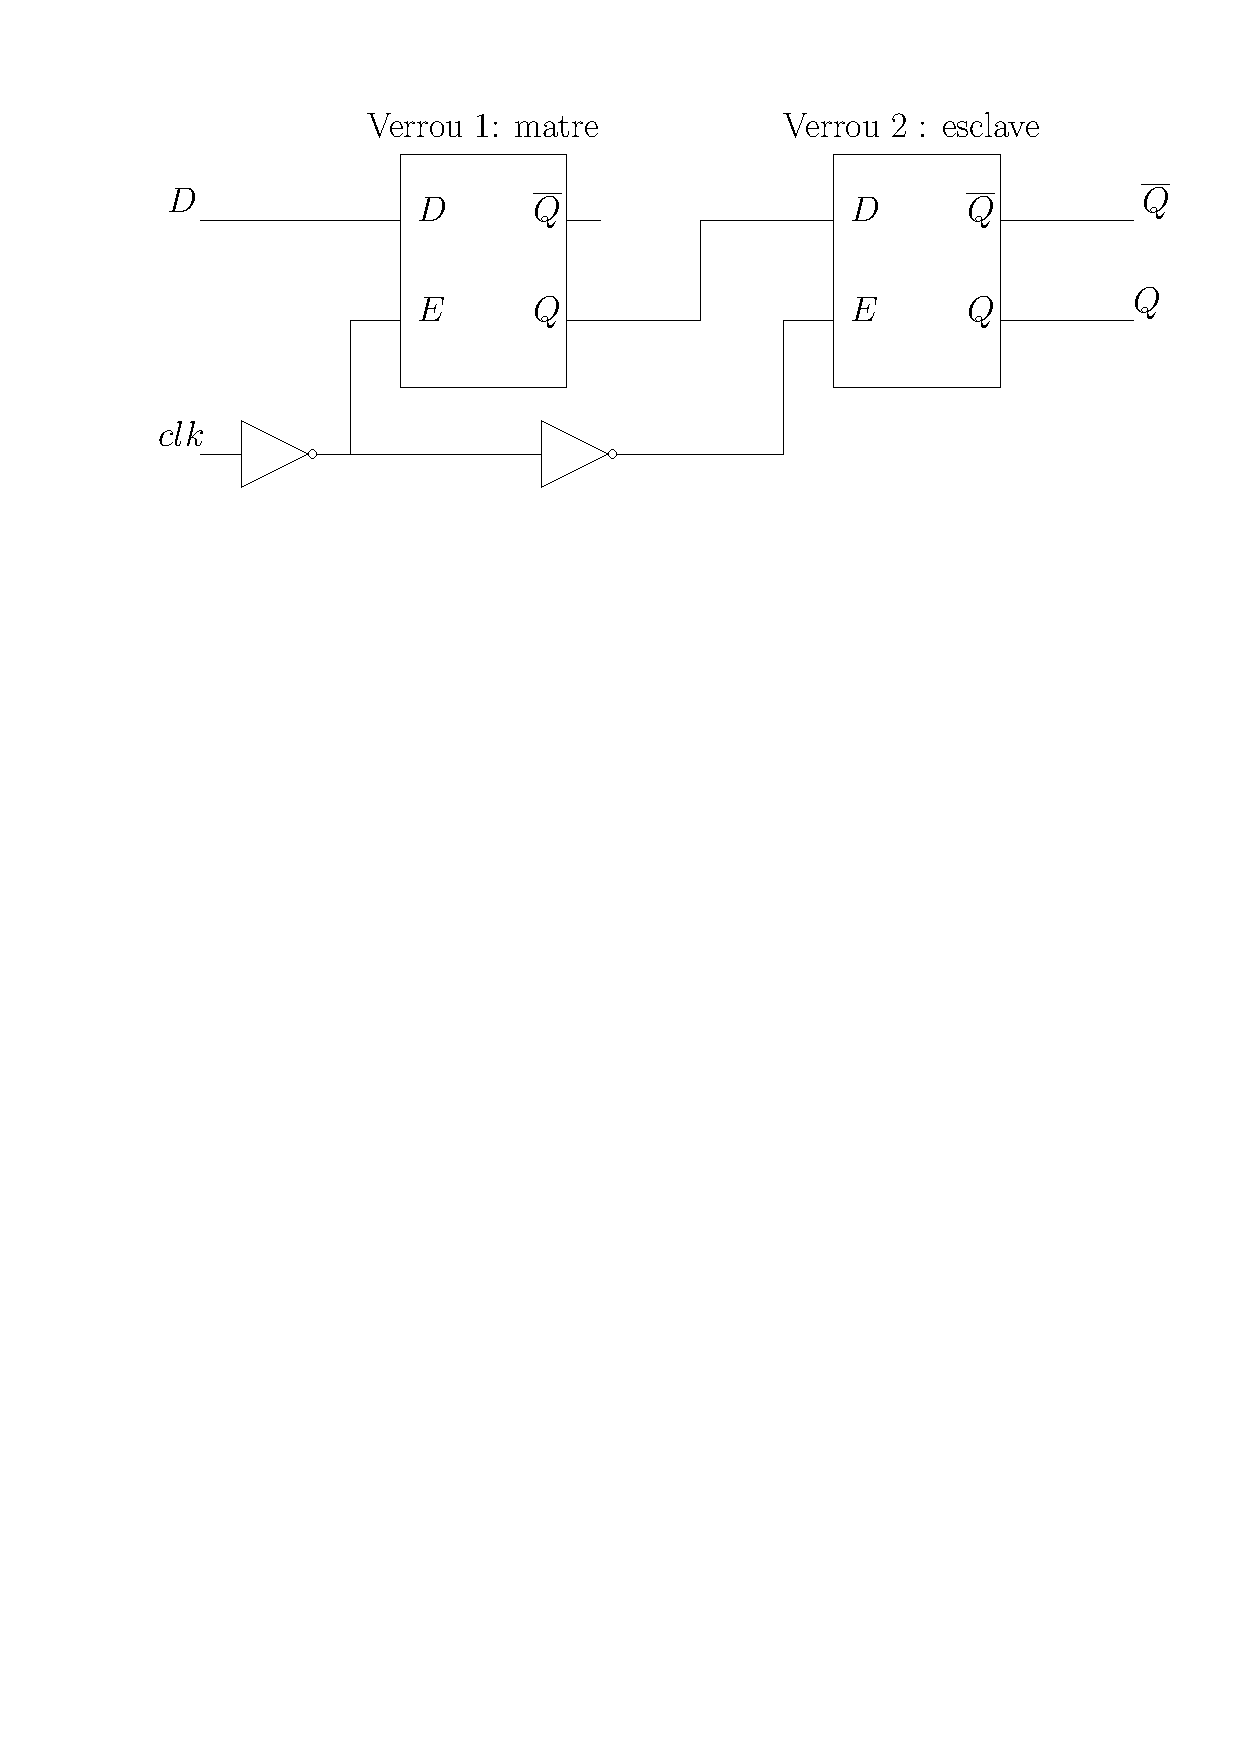
\includegraphics[width=\columnwidth]{Figs/flipflop_D.pdf}\\
\centering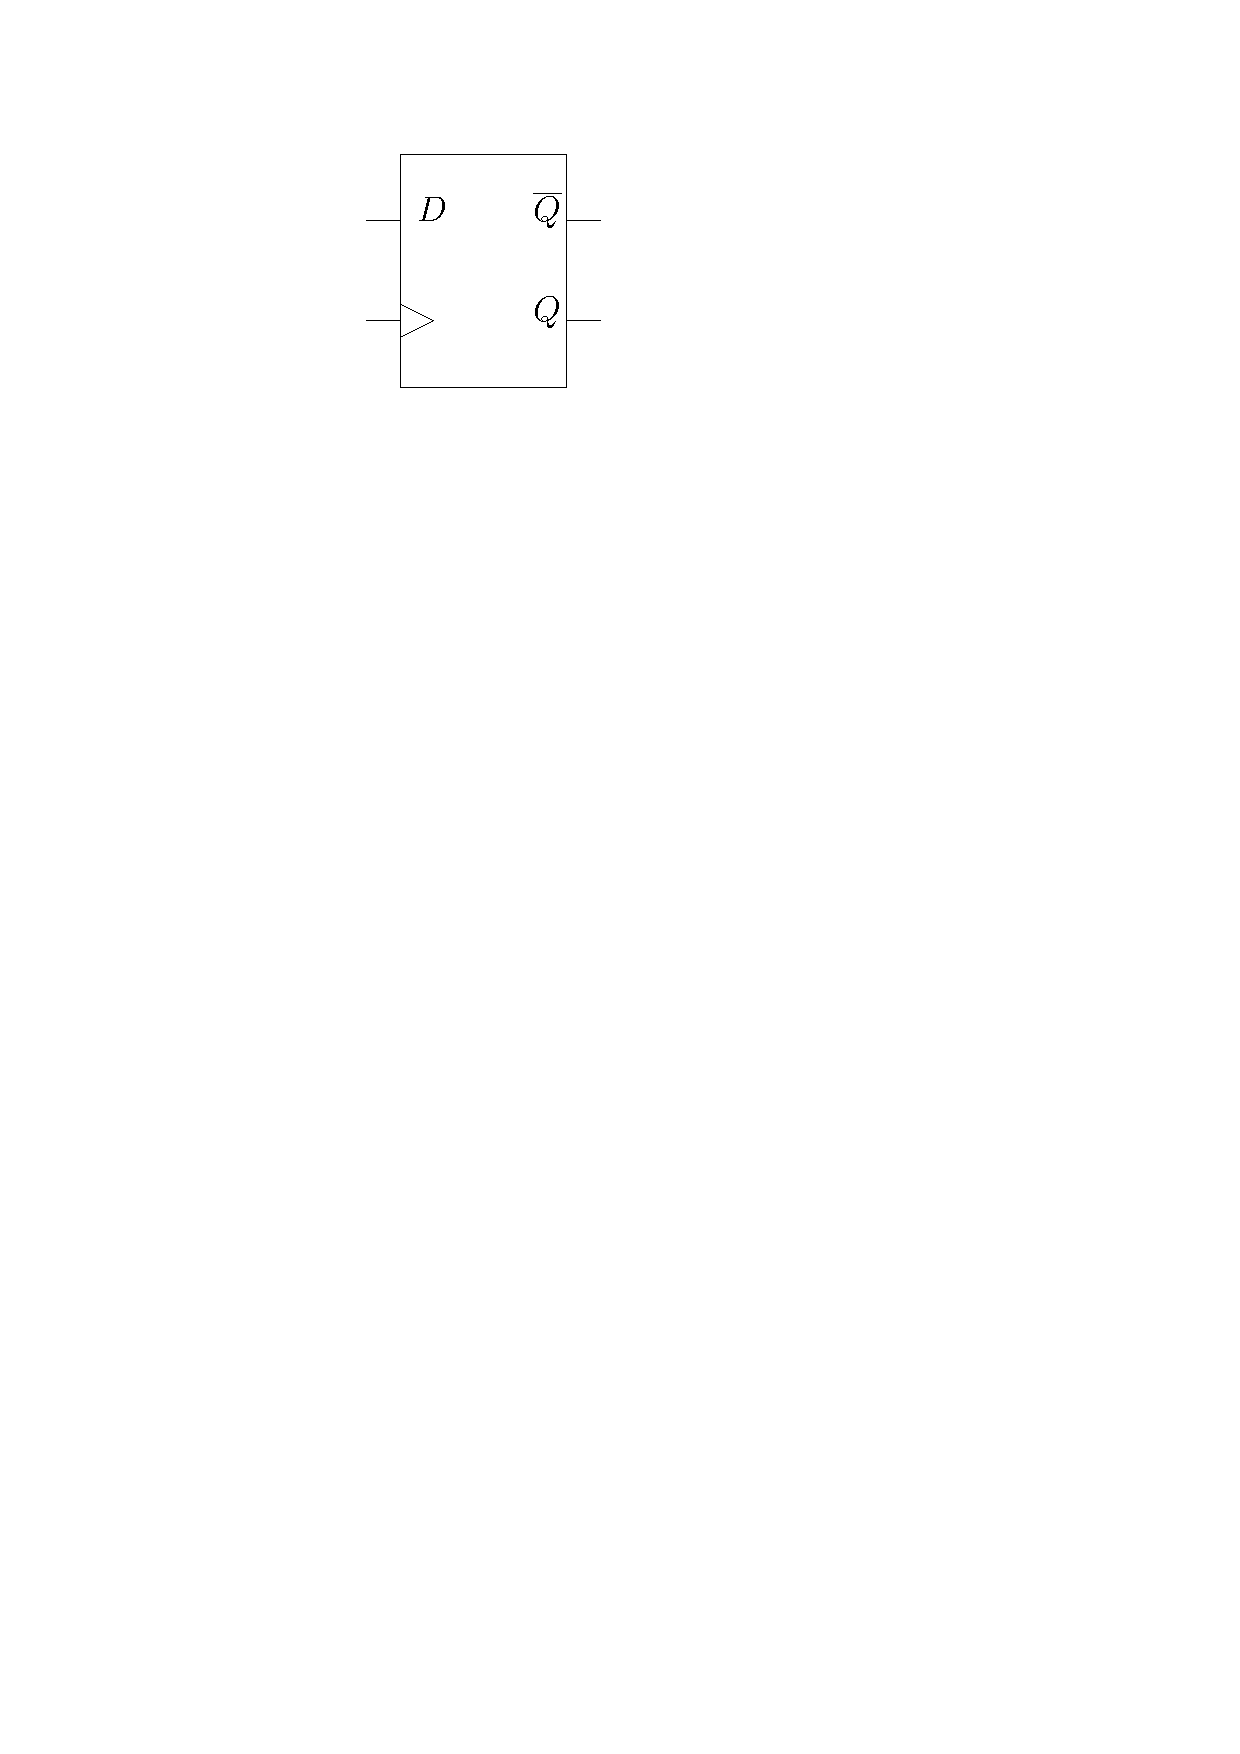
\includegraphics[width=0.3\columnwidth]{Figs/flipflop_D_schema.pdf}
\end{minipage}
\hspace{0.3cm}
 \begin{minipage}[c]{.5\linewidth}
\begin{tikztimingtable}[
    timing/coldist=2pt,     % column distance
    xscale=0.5,yscale=1, % scale diagrams
    semithick               % set line width
]
$Horloge$ & 8L 8H 8L 8H \\
$D=D_1$       & 2L 3H 2L 2H  1L 2H 1L 1H 1L 3H  6L   2L 3H 3L \\
$E_1$     & 8H 8L 8H 8L\\
$Q_1=D_2$     & 2L 3H 2L 1H 8H 2H 6L 8L\\
$E_2$     & 8L 8H 8L 8H\\
$Q=Q_2$       & 8L 8H 8H 8L\\
\extracode
  %\tablerules
  %\tablegrid
\end{tikztimingtable}
\end{minipage}
\end{block}
$Q=D$ au front montant d'horloge
\end{frame}

\begin{frame}
\frametitle{Registre à $n$ bits}

   \begin{minipage}[c]{.2\linewidth}
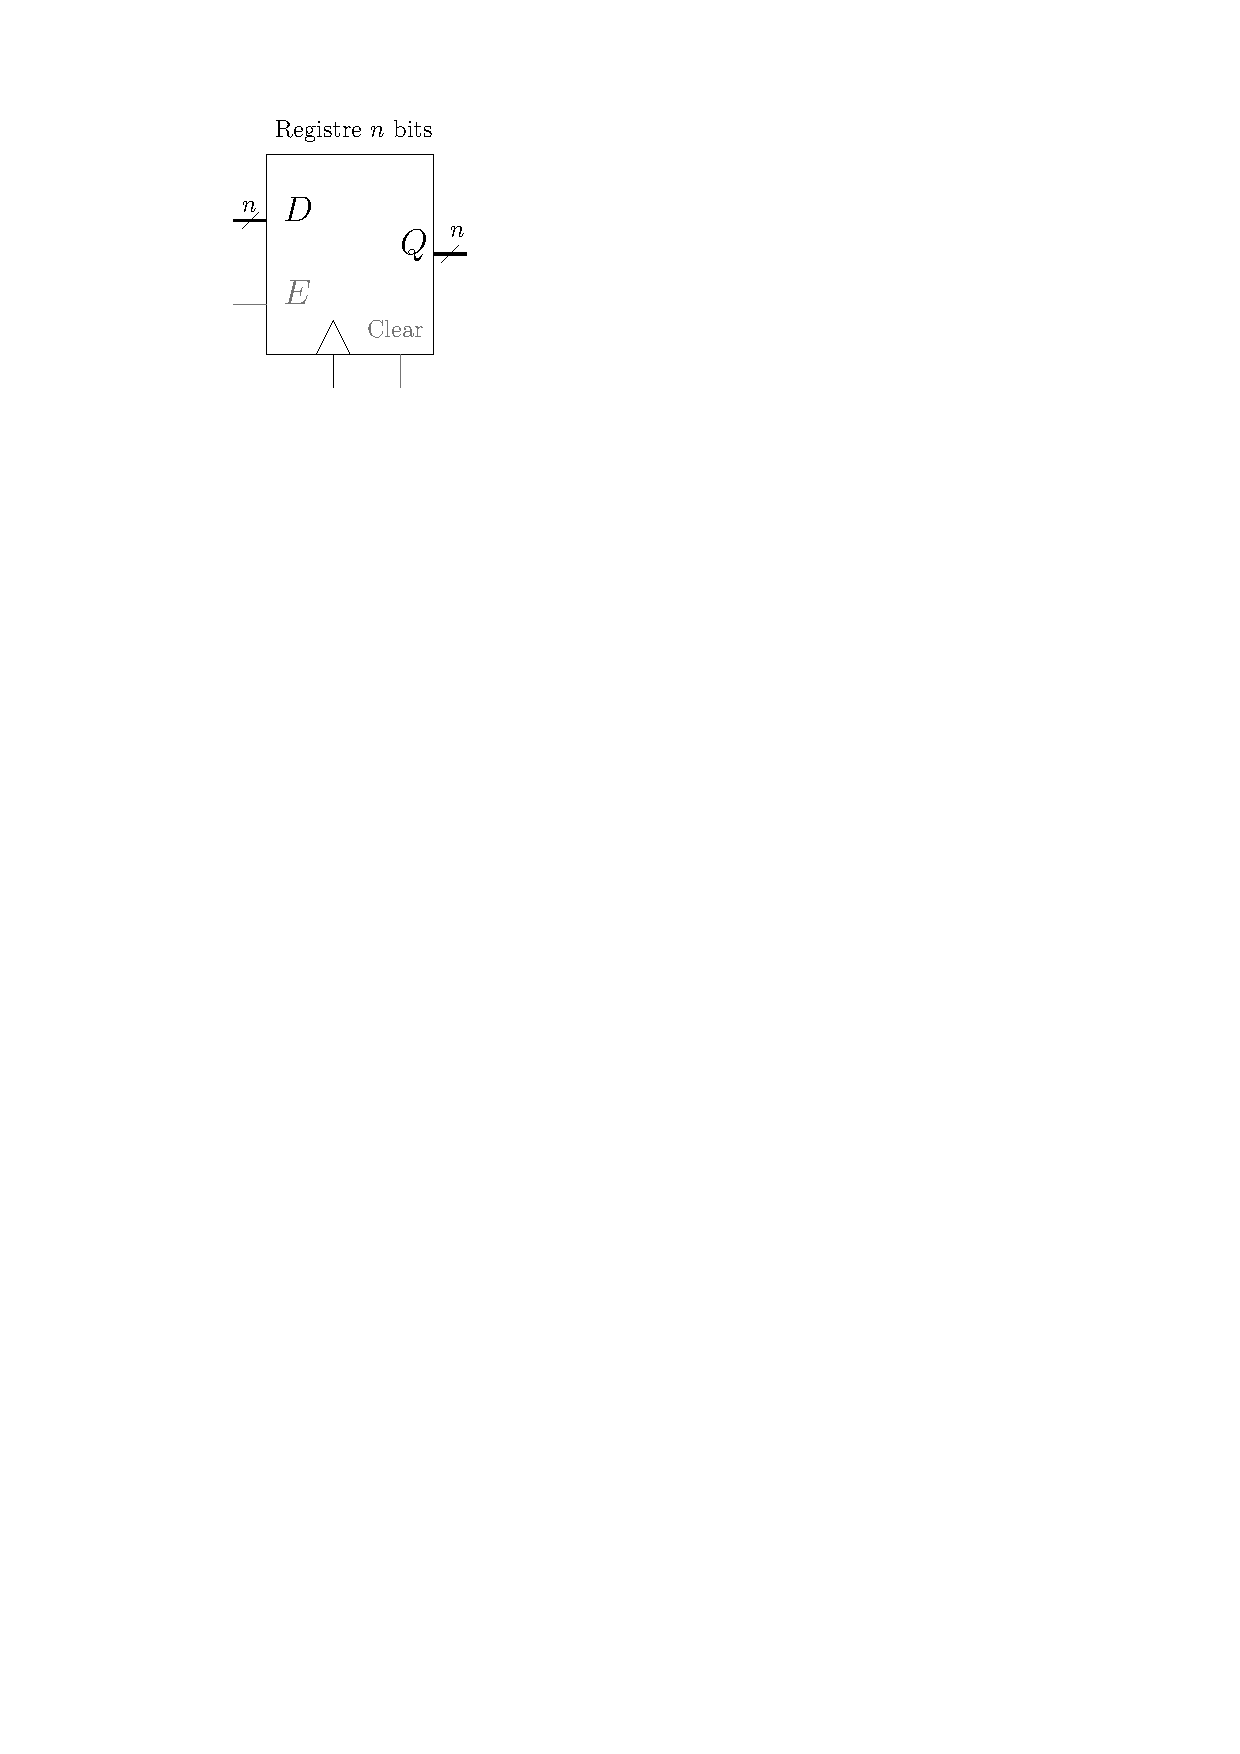
\includegraphics[width=\columnwidth]{Figs/registre.pdf}
\end{minipage}\hfill
\begin{minipage}[c]{.4\linewidth}
\includegraphics[width=\columnwidth]{Figs/registre_inner.pdf}
\end{minipage}

\end{frame}

\begin{frame}
\frametitle{Mémoire en lecture/écriture à accès aléatoire (RAM)}

\begin{minipage}[c]{.4\linewidth}
\includegraphics[width=\columnwidth]{Figs/ram.pdf}
\end{minipage}\hfill
\begin{minipage}[c]{.4\linewidth}
\includegraphics[width=\columnwidth]{Figs/ram_inner.pdf}
\end{minipage}

\begin{itemize}
\item Lecture : on place Adr et Load=1 $\Rightarrow$ $D_o$ = RAM[Adr]
\item Écriture : on place Adr, $D_i$ et Store=1 + \textbf{front d'horloge} $\Rightarrow$ RAM[Adr] = $D_{i}$
\end{itemize}

\end{frame}



%%%%%%%%%%%%%%%%%%%%%%%%%%%%
\subsection{Synthèse : notre premier chemin de données}

\begin{frame}
\frametitle{Résumons}
\begin{block}{Logique combinatoire}
\centering\includegraphics[width=\linewidth]{Figs/circuits_logique_combinatoire.pdf}
\end{block}
\begin{block}{Logique séquentielle}
\centering\includegraphics[width=0.65\linewidth]{Figs/circuits_logique_sequentielle.pdf}
\end{block}
\end{frame}


\begin{frame}
\begin{center}
\textbf{Notre premier chemin de données}
\end{center}
\end{frame}



\begin{frame}
\frametitle{Notre premier chemin de données}

\centering\includegraphics[width=0.9\columnwidth]{Figs/premier_chemin.pdf}

\begin{tiny}
\begin{block}{Spécifications}
- données et adresses sur 16 bits; RAM : $2^{16}$ mots de 16 bits = 128 ko\\
- des registres génériques : A, B ; des registres particuliers PC et RADM\\
- RAM pour stocker (pour le moment) les données\\
- des signaux de contrôle : Read$<$A,B,PC,Mem$>$, Set$<$A,B,PC,RADM,Mem$>$, UAL\\
- Architecture Load/Store : opérations avec des opérandes en registre
\end{block}
\end{tiny}
\end{frame}

\begin{frame}
\frametitle{Les registres}

\centering\includegraphics[width=0.9\columnwidth]{Figs/premier_chemin.pdf}
\begin{itemize}
\item A, B : registres d'opérandes pour effectuer des opérations
\item PC (\emph{Program counter}, ou CO : compteur ordinal): index la position de la donnée en cours d'utilisation
\item RADM : Registre d'Adresse Mémoire : quel mot est adressé en mémoire ($\neq$ PC)
\end{itemize}
\end{frame}

\begin{frame}
\frametitle{Exemple de séquencement manuel}
\begin{block}{Problème}
Additionner 16=0x0010 et 1=0x0001 et stocker le résultat à l'adresse 0x000A\\
\centering\begin{tabular}{l|cccc}
Adresses & \multicolumn{4}{c}{Contenu}\\
\hline
0000 & 0010 & 0001 & 000A & 0000\\
0004 & 0000 & 0000 & 0000 & 0000\\
0008 & 0000 & 0000 & 0000 & 0000
\end{tabular}
\end{block}
\end{frame}

\begin{frame}
\frametitle{Chargement immédiat dans A (1/3)}
\centering\includegraphics[width=\linewidth]{Figs/premier_chemin_lda_1.pdf}
\end{frame}
\begin{frame}
\frametitle{Chargement immédiat dans A (2/3)}
\centering\includegraphics[width=\linewidth]{Figs/premier_chemin_lda_2.pdf}
\end{frame}
\begin{frame}
\frametitle{Chargement immédiat dans A (3/3)}
\centering\includegraphics[width=\linewidth]{Figs/premier_chemin_lda_3.pdf}
\end{frame}

\begin{frame}
\frametitle{Chargement immédiat dans B (1/3)}
\centering\includegraphics[width=\linewidth]{Figs/premier_chemin_ldb_1.pdf}
\end{frame}
\begin{frame}
\frametitle{Chargement immédiat dans B (2/3)}
\centering\includegraphics[width=\linewidth]{Figs/premier_chemin_ldb_2.pdf}
\end{frame}
\begin{frame}
\frametitle{Chargement immédiat dans B (3/3)}
\centering\includegraphics[width=\linewidth]{Figs/premier_chemin_ldb_3.pdf}
\end{frame}

\begin{frame}
\frametitle{Addition : A := A + B}
\centering\includegraphics[width=\linewidth]{Figs/premier_chemin_adda.pdf}
\end{frame}

\begin{frame}
\frametitle{Sauvegarde du contenu du registre A en mémoire (1/4)}
\includegraphics[width=\linewidth]{Figs/premier_chemin_sta1.pdf}
\end{frame}
\begin{frame}
\frametitle{Sauvegarde du contenu du registre A en mémoire (2/4)}
\includegraphics[width=\linewidth]{Figs/premier_chemin_sta2.pdf}
\end{frame}
\begin{frame}
\frametitle{Sauvegarde du contenu du registre A en mémoire (3/4)}
\includegraphics[width=\linewidth]{Figs/premier_chemin_sta3.pdf}
\end{frame}
\begin{frame}
\frametitle{Sauvegarde du contenu du registre A en mémoire (4/4)}
\includegraphics[width=\linewidth]{Figs/premier_chemin_sta4.pdf}
\end{frame}


\begin{frame}
\frametitle{Chargement et Mode d'adressage immédiat / direct}
\begin{itemize}
\item Adressage immédiat : le \textbf{mot mémoire est la valeur} à charger
\item Adressage direct : le \textbf{mot mémoire est l'adresse} en mémoire de la valeur à charger, e.g. incrémenter un compteur dont la valeur courante est stockée à une adresse donnée en mémoire
\item Adressage indirect : le mot mémoire est l'adresse à laquelle trouver l'adresse de la valeur à charger
\item Adressage relatif : le mot mémoire contient l'adresse et un déclage, e.g. accéder aux éléments d'un tableau A[i]
\end{itemize}
\end{frame}



%%%%%%%%%%%%%%%%%%%%%%%%%%%
%%%%%%%%%%%%%%%%%%%%%%%%%%%
\section{La couche ISA}

\begin{frame}
\begin{center}
\textbf{La couche ISA (Instruction Set Architecture)}\\
\centering\includegraphics[width=0.4\linewidth]{Figs/couches_architecture.pdf}
\end{center}
\end{frame}


\begin{frame}
\frametitle{Approche par couches d'abstractions successives}
\centering\includegraphics[width=0.3\linewidth]{Figs/couches_architecture.pdf}\\
\hfill
\centering\includegraphics[width=\linewidth]{Figs/couches_architecture_specif.pdf}
\end{frame}

\begin{frame}
\frametitle{En plus des données, définissons le programme}
Architecture de von Neumann : mémoire (data+prog) $\leftrightarrow$ processeur 
\begin{block}{Les instructions}
\centering\begin{tabular}{l|cccc}
Adresses & \multicolumn{4}{c}{Contenu}\\
\hline
0000 & 0010 & 0001 & 000A & 0000\\
0004 & 0000 & 0000 & 0000 & 0000\\
0008 & 0000 & 0000 & 0000 & 0000
\end{tabular}
\end{block}
\end{frame}

\begin{frame}
\frametitle{En plus des données, définissons le programme}
Architecture de von Neumann : mémoire (data+prog) $\leftrightarrow$ processeur 
\begin{block}{Les instructions}

\centering\begin{tabular}{l|cccc}
Adresses & \multicolumn{4}{c}{Contenu}\\
\hline
0000 & LDAi & 0010 & LDBi & 0001 \\
0004 & ADDA & STA & 000A & 0000\\
0008 & 0000 & 0000 & 0000 & 0000
\end{tabular}
\end{block}
\end{frame}

\begin{frame}
\frametitle{En plus des données, définissons le programme}

\begin{block}{Codage des instructions}
\begin{tabular}{cc}
\begin{tiny}
\begin{tabular}{c|c}
Nom de l'instruction & Code de l'instruction \\
\hline
LDAi & $0\times1000$\\
LDAd & $0\times1400$\\
LDBi & $0\times2000$\\
STA  & $0\times1c00$\\
ADDA & $0\times3000$
\end{tabular}\end{tiny}&
\begin{footnotesize}\begin{tabular}{l|cccc}
Adresses & \multicolumn{4}{c}{Contenu}\\
\hline
0000 & 1000 & 0010 & 2000 & 0001\\
0004 & 3000 & 1c00 & 000A & 0000\\
0008 & 0000 & 0000 & 0000 & 0000
\end{tabular}\end{footnotesize}
\end{tabular}
\end{block}
$\Rightarrow$ Programme en \textbf{langage machine}
\end{frame}

\begin{frame}
\frametitle{Récupérer l'instruction (fetch)}
\begin{block}{Une première possibilité}
\includegraphics[width=\linewidth]{Figs/premier_chemin_ri.pdf}\\
L'instruction est :
\begin{itemize}
\item récupérée en mémoire
\item placée dans le registre d'instruction (RI)
\item qui est une entrée du séquenceur
\end{itemize}
\end{block}
\end{frame}

\begin{frame}
\frametitle{Séquencement du chemin de données}
\begin{block}{Séquenceur}
Séquence de signaux de contrôle spécifique :
\begin{enumerate}
\item pour récupérer l'instruction 
\item en fonction de l'instruction
\end{enumerate}
$\Rightarrow$ machine à états finis
\end{block}
\end{frame}

\begin{frame}
\frametitle{Générer les signaux de contrôle : le séquenceur}
\begin{block}{Fetch}
\includegraphics[width=\linewidth]{Figs/premier_chemin_ri.pdf}\\
  \centering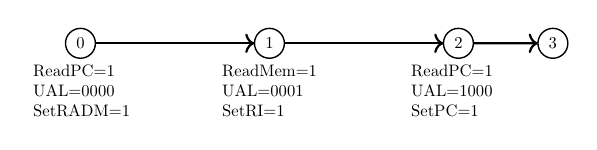
\begin{tikzpicture}[scale=0.6, every node/.style={scale=0.6}]
    GraphInit[vstyle=Normal]
    \SetGraphUnit{3}
    \tikzset{LabelStyle/.style= {draw,
        fill  = yellow,
        text  = red},
      EdgeStyle/.style = {->}}
    \Vertex[Math,L=0,x=0,y=2]{A}
    \Vertex[Math,L=1,x=4,y=2]{B}
    \Vertex[Math,L=2,x=8,y=2]{C}
    \Vertex[Math,L=3,x=10,y=2]{D}
    \Edge(A)(B)
    \Edge(B)(C)
    \Edge(C)(D)
    \node[text width=2cm] at ($(A) - (0,1)$) {ReadPC=1\\UAL=0000\\SetRADM=1} ;
    \node[text width=2cm] at ($(B) - (0,1)$) {ReadMem=1\\UAL=0001\\SetRI=1} ;
    \node[text width=2cm] at ($(C) - (0,1)$) {ReadPC=1\\UAL=1000\\SetPC=1} ;
  \end{tikzpicture}
\end{block}
\end{frame}

\begin{frame}
\frametitle{Générer les signaux de contrôle : le séquenceur}
\begin{block}{Chargement immédiat dans A : LDAi}
\includegraphics[width=\linewidth]{Figs/premier_chemin_ri.pdf}\\
  \centering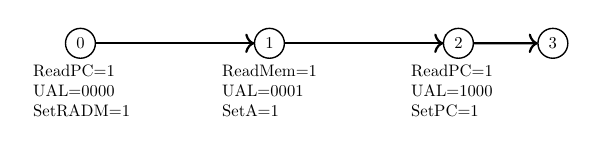
\begin{tikzpicture}[scale=0.6, every node/.style={scale=0.6}]
    GraphInit[vstyle=Normal]
    \SetGraphUnit{3}
    \tikzset{LabelStyle/.style= {draw,
        fill  = yellow,
        text  = red},
      EdgeStyle/.style = {->}}
    \Vertex[Math,L=0,x=0,y=2]{A}
    \Vertex[Math,L=1,x=4,y=2]{B}
    \Vertex[Math,L=2,x=8,y=2]{C}
    \Vertex[Math,L=3,x=10,y=2]{D}
    \Edge(A)(B)
    \Edge(B)(C)
    \Edge(C)(D)
    \tikzset{VertexStyle/.append style={rectangle}}
    \node[text width=2cm] at ($(A) - (0,1)$) {ReadPC=1\\UAL=0000\\SetRADM=1} ;
    \node[text width=2cm] at ($(B) - (0,1)$) {ReadMem=1\\UAL=0001\\SetA=1} ;
    \node[text width=2cm] at ($(C) - (0,1)$) {ReadPC=1\\UAL=1000\\SetPC=1} ;
  \end{tikzpicture}
\end{block}
\end{frame}

\begin{frame}
\frametitle{Générer les signaux de contrôle : le séquenceur}
\begin{block}{Chargement immédiat dans B : LDBi}
\includegraphics[width=\linewidth]{Figs/premier_chemin_ri.pdf}\\
  \centering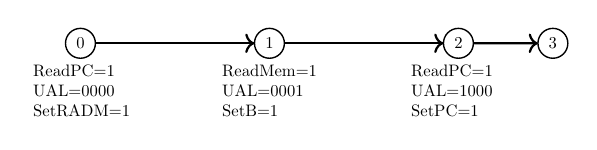
\begin{tikzpicture}[scale=0.6, every node/.style={scale=0.6}]
    GraphInit[vstyle=Normal]
    \SetGraphUnit{3}
    \tikzset{LabelStyle/.style= {draw,
        fill  = yellow,
        text  = red},
      EdgeStyle/.style = {->}}
    \Vertex[Math,L=0,x=0,y=2]{A}
    \Vertex[Math,L=1,x=4,y=2]{B}
    \Vertex[Math,L=2,x=8,y=2]{C}
    \Vertex[Math,L=3,x=10,y=2]{D}
    \Edge(A)(B)
    \Edge(B)(C)
    \Edge(C)(D)
    \tikzset{VertexStyle/.append style={rectangle}}
    \node[text width=2cm] at ($(A) - (0,1)$) {ReadPC=1\\UAL=0000\\SetRADM=1} ;
    \node[text width=2cm] at ($(B) - (0,1)$) {ReadMem=1\\UAL=0001\\SetB=1} ;
    \node[text width=2cm] at ($(C) - (0,1)$) {ReadPC=1\\UAL=1000\\SetPC=1} ;
  \end{tikzpicture}
\end{block}
\end{frame}


\begin{frame}
\frametitle{Générer les signaux de contrôle : le séquenceur}
\begin{block}{Chargement direct dans A : LDAd}
\includegraphics[width=\linewidth]{Figs/premier_chemin_ri.pdf}\\
\centering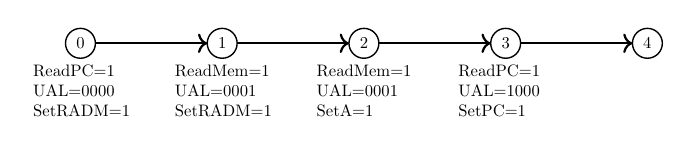
\begin{tikzpicture}[scale=0.6, every node/.style={scale=0.6}]
    GraphInit[vstyle=Normal]
    \SetGraphUnit{3}
    \tikzset{LabelStyle/.style= {draw,
        fill  = yellow,
        text  = red},
      EdgeStyle/.style = {->}}
    \Vertex[Math,L=0,x=0,y=2]{A}
    \Vertex[Math,L=1,x=3,y=2]{B}
    \Vertex[Math,L=2,x=6,y=2]{C}
    \Vertex[Math,L=3,x=9,y=2]{D}
    \Vertex[Math,L=4,x=12,y=2]{E}
    \Edge(A)(B)
    \Edge(B)(C)
    \Edge(C)(D)
    \Edge(D)(E)
    \node[text width=2cm] at ($(A) - (0,1)$) {ReadPC=1\\UAL=0000\\SetRADM=1} ;
    \node[text width=2cm] at ($(B) - (0,1)$) {ReadMem=1\\UAL=0001\\SetRADM=1} ;
    \node[text width=2cm] at ($(C) - (0,1)$) {ReadMem=1\\UAL=0001\\SetA=1} ;
    \node[text width=2cm] at ($(D) - (0,1)$) {ReadPC=1\\UAL=1000\\SetPC=1} ;
  \end{tikzpicture}
\end{block}
\end{frame}

\begin{frame}
\frametitle{Générer les signaux de contrôle : le séquenceur}
\begin{block}{Addition A:= A + B : ADDA}
\includegraphics[width=\linewidth]{Figs/premier_chemin_ri.pdf}\\
  \centering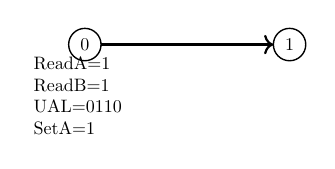
\begin{tikzpicture}[scale=0.65, every node/.style={scale=0.65}]
    GraphInit[vstyle=Normal]
    \SetGraphUnit{3}
    \tikzset{LabelStyle/.style= {draw,
        fill  = yellow,
        text  = red},
      EdgeStyle/.style = {->}}
    \Vertex[Math,L=0,x=0,y=2]{A}
    \Vertex[Math,L=1,x=4,y=2]{B}
    \Edge(A)(B)
    \node[text width=2cm] at ($(A) - (0,1)$) {ReadA=1\\ReadB=1\\UAL=0110\\SetA=1} ;
  \end{tikzpicture}
\end{block}
\end{frame}

\begin{frame}
\frametitle{Générer les signaux de contrôle : le séquenceur}
\begin{block}{Sauvegarde de A en mémoire : STA}
\includegraphics[width=\linewidth]{Figs/premier_chemin_ri.pdf}\\
  \centering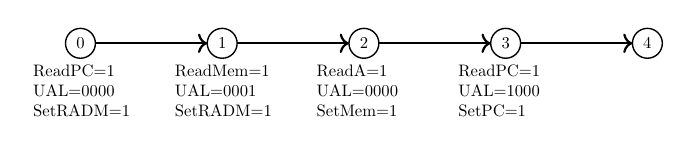
\begin{tikzpicture}[scale=0.6, every node/.style={scale=0.6}]
    GraphInit[vstyle=Normal]
    \SetGraphUnit{3}
    \tikzset{LabelStyle/.style= {draw,
        fill  = yellow,
        text  = red},
      EdgeStyle/.style = {->}}
    \Vertex[Math,L=0,x=0,y=2]{A}
    \Vertex[Math,L=1,x=3,y=2]{B}
    \Vertex[Math,L=2,x=6,y=2]{C}
    \Vertex[Math,L=3,x=9,y=2]{D}
    \Vertex[Math,L=4,x=12,y=2]{E}
    \Edge(A)(B)
    \Edge(B)(C)
    \Edge(C)(D)
    \Edge(D)(E)
    \tikzset{VertexStyle/.append style={rectangle}}
    \node[text width=2cm] at ($(A) - (0,1)$) {ReadPC=1\\UAL=0000\\SetRADM=1} ;
    \node[text width=2cm] at ($(B) - (0,1)$) {ReadMem=1\\UAL=0001\\SetRADM=1} ;
    \node[text width=2cm] at ($(C) - (0,1)$) {ReadA=1\\UAL=0000\\SetMem=1} ;
    \node[text width=2cm] at ($(D) - (0,1)$) {ReadPC=1\\UAL=1000\\SetPC=1} ;
  \end{tikzpicture}
\end{block}
\end{frame}


\begin{frame}
\frametitle{Machine à états finis pour le séquenceur}
  \centering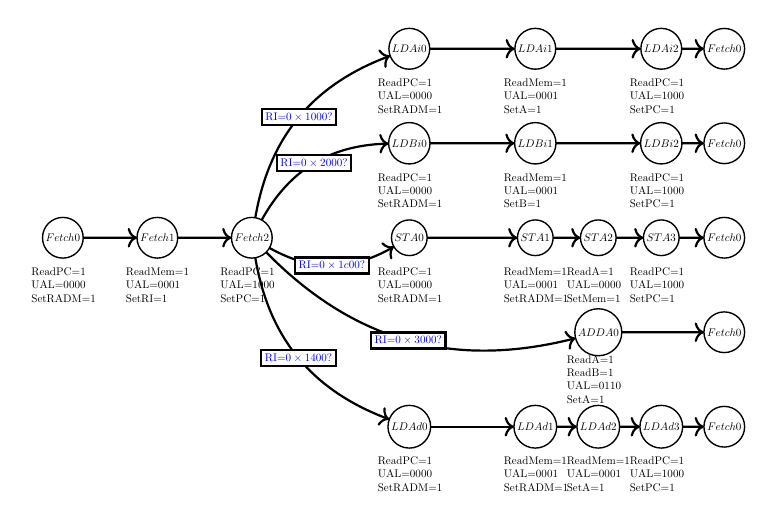
\begin{tikzpicture}[thick,scale=0.4, every node/.style={scale=0.4}]
    GraphInit[vstyle=Normal]
    \SetGraphUnit{3}
    \tikzset{LabelStyle/.style= {draw,
        fill  = white,
        text  = blue},
      EdgeStyle/.style = {->}}
    \Vertex[Math,L=Fetch0,x=-11,y=8]{A0}
    \Vertex[Math,L=Fetch1,x=-8,y=8]{B0}
    \Vertex[Math,L=Fetch2,x=-5,y=8]{C0}
    \Edge(A0)(B0)
    \Edge(B0)(C0)
    \node[text width=2cm] at ($(A0) - (0,1.5)$) {ReadPC=1\\UAL=0000\\SetRADM=1} ;
    \node[text width=2cm] at ($(B0) - (0,1.5)$) {ReadMem=1\\UAL=0001\\SetRI=1} ;
    \node[text width=2cm] at ($(C0) - (0,1.5)$) {ReadPC=1\\UAL=1000\\SetPC=1} ;


    \Vertex[Math,L=LDAi0,x=0,y=14]{A1}
    \Vertex[Math,L=LDAi1,x=4,y=14]{B1}
    \Vertex[Math,L=LDAi2,x=8,y=14]{C1}
    \Vertex[Math,L=Fetch0,x=10,y=14]{D1}
    \Edge(A1)(B1)
    \Edge(B1)(C1)
    \Edge(C1)(D1)
    \node[text width=2cm] at ($(A1) - (0,1.5)$) {ReadPC=1\\UAL=0000\\SetRADM=1} ;
    \node[text width=2cm] at ($(B1) - (0,1.5)$) {ReadMem=1\\UAL=0001\\SetA=1} ;
    \node[text width=2cm] at ($(C1) - (0,1.5)$) {ReadPC=1\\UAL=1000\\SetPC=1} ;

    \Vertex[Math,L=LDBi0,x=0,y=11]{A2}
    \Vertex[Math,L=LDBi1,x=4,y=11]{B2}
    \Vertex[Math,L=LDBi2,x=8,y=11]{C2}
    \Vertex[Math,L=Fetch0,x=10,y=11]{D2}
    \Edge(A2)(B2)
    \Edge(B2)(C2)
    \Edge(C2)(D2)
    \node[text width=2cm] at ($(A2) - (0,1.5)$) {ReadPC=1\\UAL=0000\\SetRADM=1} ;
    \node[text width=2cm] at ($(B2) - (0,1.5)$) {ReadMem=1\\UAL=0001\\SetB=1} ;
    \node[text width=2cm] at ($(C2) - (0,1.5)$) {ReadPC=1\\UAL=1000\\SetPC=1} ;


    \Vertex[Math,L=STA0,x=0,y=8]{A3}
    \Vertex[Math,L=STA1,x=4,y=8]{B3}
    \Vertex[Math,L=STA2,x=6,y=8]{C3}
    \Vertex[Math,L=STA3,x=8,y=8]{D3}
    \Vertex[Math,L=Fetch0,x=10,y=8]{E3}
    \Edge(A3)(B3)
    \Edge(B3)(C3)
    \Edge(C3)(D3)
    \Edge(D3)(E3)
    \node[text width=2cm] at ($(A3) - (0,1.5)$) {ReadPC=1\\UAL=0000\\SetRADM=1} ;
    \node[text width=2cm] at ($(B3) - (0,1.5)$) {ReadMem=1\\UAL=0001\\SetRADM=1} ;
    \node[text width=2cm] at ($(C3) - (0,1.5)$) {ReadA=1\\UAL=0000\\SetMem=1} ;
    \node[text width=2cm] at ($(D3) - (0,1.5)$) {ReadPC=1\\UAL=1000\\SetPC=1} ;




    \Vertex[Math,L=ADDA0,x=6,y=5]{A4}
    \Vertex[Math,L=Fetch0,x=10,y=5]{B4}
    \Edge(A4)(B4)
    \node[text width=2cm] at ($(A4) - (0,1.5)$) {ReadA=1\\ReadB=1\\UAL=0110\\SetA=1} ;

    \Vertex[Math,L=LDAd0,x=0,y=2]{A5}
    \Vertex[Math,L=LDAd1,x=4,y=2]{B5}
    \Vertex[Math,L=LDAd2,x=6,y=2]{C5}
    \Vertex[Math,L=LDAd3,x=8,y=2]{D5}
    \Vertex[Math,L=Fetch0,x=10,y=2]{E5}
    \Edge(A5)(B5)
    \Edge(B5)(C5)
    \Edge(C5)(D5)
    \Edge(D5)(E5)
    \node[text width=2cm] at ($(A5) - (0,1.5)$) {ReadPC=1\\UAL=0000\\SetRADM=1} ;
    \node[text width=2cm] at ($(B5) - (0,1.5)$) {ReadMem=1\\UAL=0001\\SetRADM=1} ;
    \node[text width=2cm] at ($(C5) - (0,1.5)$) {ReadMem=1\\UAL=0001\\SetA=1} ;
    \node[text width=2cm] at ($(D5) - (0,1.5)$) {ReadPC=1\\UAL=1000\\SetPC=1} ;


    \Edge[style={->,bend left},label={RI=$0\times1000$?}](C0)(A1)
    \Edge[style={->,bend left},label={RI=$0\times2000$?}](C0)(A2)
    \Edge[style={->,bend right},label={RI=$0\times1c00$?}](C0)(A3)
    \Edge[style={->,bend right},label={RI=$0\times3000$?}](C0)(A4)
    \Edge[style={->,bend right},label={RI=$0\times1400$?}](C0)(A5)
  \end{tikzpicture}

Réalisation matérielle ? Soyons astucieux sur le codage des états
\end{frame}

\begin{frame}
\frametitle{Séquenceur micro-programmé}
\centering\includegraphics[width=\linewidth]{Figs/sequenceur_micro.pdf}
\end{frame}

\begin{frame}
\frametitle{Notre première architecture interne}
\centering\includegraphics[width=\linewidth]{Figs/premier_chemin_seq.pdf}
\end{frame}

\begin{frame}
\frametitle{Les micro-instructions}
\centering\includegraphics[width=0.6\linewidth]{Figs/sequenceur_micro.pdf}\\

\begin{small}
\begin{itemize}
\item ROM[0x00] : saut à fetch
\item ROM[0x08,0x09,0x0A,0x0B] : fetch/decode
\item ROM[0x10,0x11,0x12,0x13] : LDAi
\item ROM[0x14,0x15,0x16,0x17] : LDAd
\item ROM[0x1c,0x1d,0x1e,0x1f] : LDAd
\item ROM[0x20,0x21,0x22,0x23] : LDBi
\item ROM[0x30,0x31,0x32,0x33] : ADDA
\end{itemize}
\end{small}
\end{frame}

\begin{frame}
\frametitle{Les branchements}
\begin{eqnarray*}
fact(n) = \begin{cases}
\mbox{si } n=0 \mbox{ alors}& 1\\
\mbox{sinon }& n * fact(n-1)
\end{cases}
\end{eqnarray*}
si ... alors ... sinon ? Indicateurs de l'UAL
\begin{block}{Instructions de branchement}
\begin{footnotesize}
\begin{itemize}
\item \texttt{JMP} ($0\times7000$)
\begin{eqnarray*}
\texttt{JMP op} \Leftrightarrow PC := op
\end{eqnarray*}
\item \texttt{JZA}  ($0\times7400$)
\begin{eqnarray*}
\texttt{JZA op}  \Leftrightarrow \begin{cases}
PC := op & \mbox{si } A==0\\
PC := PC+1 & \mbox{sinon}
\end{cases}
\end{eqnarray*}
\item \texttt{JZB}  ($0\times7800$)
\end{itemize}
\end{footnotesize}
\end{block}

\end{frame}

\begin{frame}
\frametitle{Architecture avec branchement}
\centering\includegraphics[width=\linewidth]{Figs/premier_chemin_seq_jmp.pdf}
\end{frame}

\begin{frame}
\frametitle{Architecture avec branchement}
\centering\includegraphics[width=0.6\linewidth]{Figs/premier_chemin_seq_jmp.pdf}\\
\begin{scriptsize}
\begin{tabular}{cc|cr}
CodeMCount & Z & $S_1S_0$ & Sémantique\\
\hline
000 &  0 ou 1 & 00 & MicroPC := MicroPC+1\\
001 &  0 ou 1 & 01 & MicroPC := @Adr\\
010 &  0 ou 1 & 10 & MicroPC := Instruction\\
011 &  0 & 00 & MicroPC := MicroPC+1  si la sortie de l'UAL $\neq 0$\\
011 &  1 & 01 & MicroPC := @Adr si la sortie de l'UAL $== 0$
\end{tabular}
\end{scriptsize}
\end{frame}


%% \section{Procédures, pile et pointeur de pile}
%% \section{Traduction, compilation, interprétation}
%% \section{Les mémoires}
%% \section{Les périphériques}
%% \section{Les interruptions}
%% \section{Suppléments}

%------------------------------------------------

%----------------------------------------------------------------------------------------

\end{document} 
